\documentclass[12pt,a4paper,portuges]{scrreprt}
%not free anymore, is this really neaded?
%\usepackage{floatflt}
\usepackage{varioref}
\usepackage{shadow}
\usepackage{footmisc}
\usepackage{include/eurotux}
%%%%%%%%%%%%%%%%%%%%%%%%%%%%%%%%%%%%%%%%%%%%%%%%
\newcommand{\acronym}{UnitBox }
\ifx\UseOption\undefined
\def\UseOption{etva}
\fi
\usepackage{optional}

% forçar numeração nas secções
\setcounter{secnumdepth}{5}
\setcounter{tocdepth}{5}

\author{Eurotux Informática, S.A.}
\title{Manual UnitBox G3 v2.1.0}
\subtitle{Eurotux Informática, S.A.}
\date{\today}
%\date{Fevereiro de 2006}

\begin{document}

\maketitle

\begin{Log}
\LogEntry{Carlos Rodrigues}{cmar@eurotux.com}{2013-12-20}
Actualização de images e release 2.1.0
\LogEntry{Carlos Rodrigues}{cmar@eurotux.com}{2013-08-22}
Sub-secção \textit{Servidor de ficheiros} da secção \textit{ETVA Management Agents}
\LogEntry{Carlos Rodrigues}{cmar@eurotux.com}{2013-08-08}
Actualização da Sub-Secção \textit{Armazenamento} com informação sobre \emph{Storage iSCSI}
\LogEntry{Carlos Rodrigues}{cmar@eurotux.com}{2013-06-12}
Actualização da Sub-Secção \textit{Primavera} da Secção \textit{Management Agents}
\LogEntry{Carlos Rodrigues}{cmar@eurotux.com}{2013-05-31}
Actualização da Sub-Secção \textit{Primavera} da Secção \textit{Management Agents}
\LogEntry{Carlos Rodrigues}{cmar@eurotux.com}{2013-05-30}
Actualização da Secção \textit{Administração de utilizadores, grupos e permissões}
\LogEntry{Carlos Rodrigues}{cmar@eurotux.com}{2013-02-11}
Actualização de algumas images, Secção \textit{Changelog} e alteração do nome para UnitBox
\LogEntry{Carlos Rodrigues}{cmar@eurotux.com}{2012-10-03}
Secção \textit{Servidores}, adicionado \textit{Snapshots}
\LogEntry{Carlos Rodrigues}{cmar@eurotux.com}{2012-10-01}
Secção \textit{Datacenter virtual}, em \textit{Editar datacenter} actualizado \textit{Nó com alta disponibilidade }
\LogEntry{Carlos Rodrigues}{cmar@eurotux.com}{2012-07-23}
Secção \textit{Datacenter virtual}, sub-secção \textit{Nodes} actualizada e \textit{rebrand} de algumas imagens para NUXIS
\LogEntry{Carlos Rodrigues}{cmar@eurotux.com}{2012-07-20}
Sub-secção \textit{Armazenamento} atualizada
\LogEntry{Carlos Rodrigues}{cmar@eurotux.com}{2012-07-13}
Sub-secção \textit{Editar máquina virtual} atualizada
\LogEntry{Manuel Dias}{mfd@eurotux.com}{2012-05-17}
Alteração do nome para NUXIS. Sub-secção \textit{Editar máquina virtual} atualizada
\LogEntry{Carlos Rodrigues}{cmar@eurotux.com}{2012-04-20}
Alteração da versão
\LogEntry{Manuel Dias}{mfd@eurotux.com}{2011-11-30}
Sub-secção \textit{Drivers virtio} da secção \textit{Máquina virtual}
\LogEntry{Manuel Dias}{mfd@eurotux.com}{2011-11-21}
Sub-secção \textit{Gestão de Datacenters Virtuais} da secção \textit{Administração do sistema}
\LogEntry{Manuel Dias}{mfd@eurotux.com}{2011-10-13}
Sub-secção Administração de utilizadores, grupos e permissões da secção \textit{Administração do sistema}
\LogEntry{Carlos Rodrigues}{cmar@eurotux.com}{2011-07-13}
Sub-secção \textit{ETFW} da secção \textit{ETVA Management Agents}
\LogEntry{Carlos Rodrigues}{cmar@eurotux.com}{2011-07-01}
Sub-secção \textit{Primavera} da secção \textit{ETVA Management Agents}
\LogEntry{Ricardo Gomes}{rjg@eurotux.com}{2010-08-06}
Versão inicial.
\end{Log}

\tableofcontents

\listoffigures

\chapter{\textsf{ETVA}}
\section{Descrição}
A \emph{Eurotux Virtual Appliance} é uma ferramenta de gestão centralizada de recursos disponíveis numa rede. Consiste numa distribuição linux pré-instalada e configurada que permite fazer a gestão via rede de servidores e seus recursos.


A ETVA encontra-se dividida principalmente em dois blocos funcionais:

\begin{itemize}
	\item \emph{Central Management} (CM)
        \item \emph{Virtualization Agent} (VA)
\end{itemize}

\begin{figure}[H]
	\begin{center}
	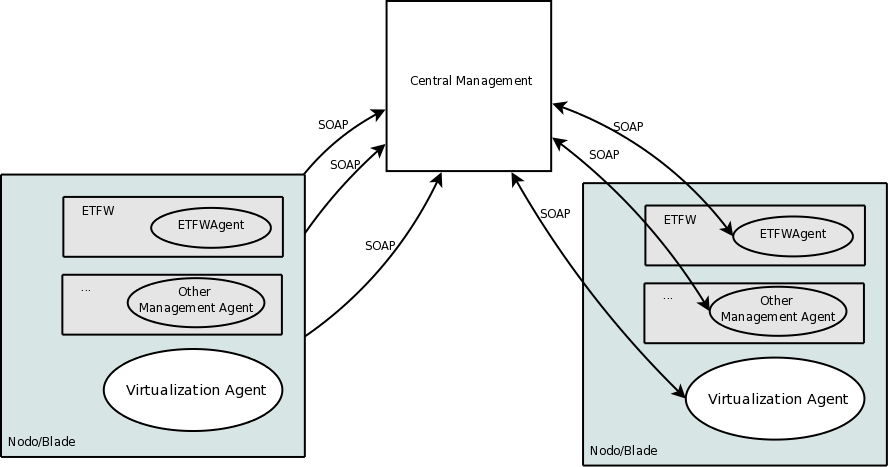
\includegraphics[scale=0.35]{screenshots/etva_blocos.png}
	\caption{Esquema geral do ETVA}
	\label{fig:etva_blocos}
	\end{center}
\end{figure}

O CM é o bloco responsável por gerir toda a infra-estrutura.
Os \emph{Virtualization Agents} são responsáveis pelo processamento dos pedidos entre os servidores de virtualização (\emph{nodes}) e o CM.

Dentro de um servidor de virtualização(\emph{node}) poderão existir máquinas virtuais com \emph{Management Agents}. Estes agentes, permitem a gestão ao nível dos serviços/aplicações instalados numa máquina virtual (ver figura \ref{fig:etva_blocos} ).

\section{Versões}

Atualmente o ETVA encontra-se disponível em duas versões:
\begin{description}
	\item[Standard -] Nesta versão, o modelo do ETVA consiste num único servidor de virtualização onde se encontram instalados o CM e o VA. A configuração da rede do \emph{node} neste modelo consistem em quatro interfaces de rede: Internet, LAN, DMZ e Management.
		\begin{figure}[H]
			\begin{center}
			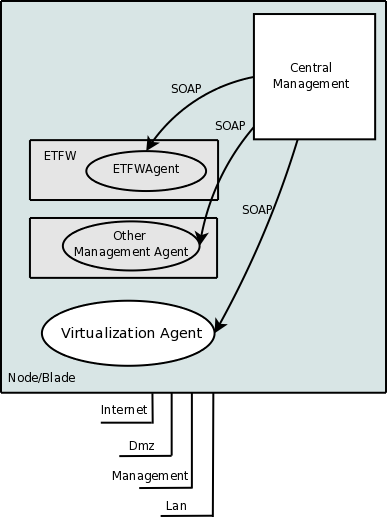
\includegraphics[scale=0.4]{screenshots/etva_standard.png}
			\caption{Modelo ETVA Standard}
			\label{fig:etva_standard}
			\end{center}
		\end{figure}
	\item[Enterprise -] Nesta versão, existem vários servidores de virtualização (\emph{nodes}) a comunicar com o CM. A configuração da rede inicial, é efectuada, com recurso a VLANs, através do \emph{Assistente de configuração inicial} conforme indica a figura \ref{fig:first_time_wizard}.
		\begin{figure}[H]
			\begin{center}
			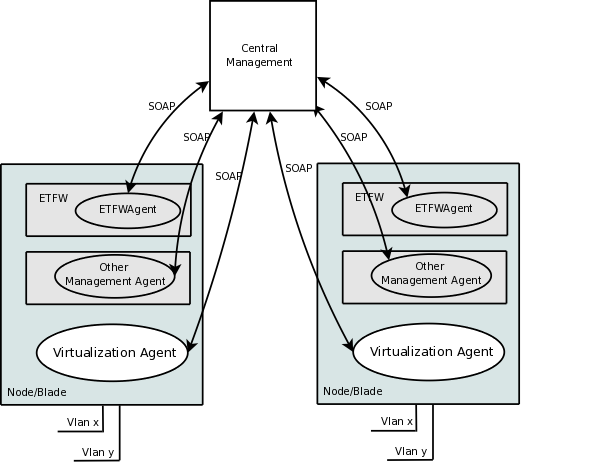
\includegraphics[scale=0.6]{screenshots/etva_enterprise.png}
			\caption{Modelo ETVA Enterprise}
			\label{fig:etva_enterprise}
			\end{center}
		\end{figure}
\end{description}
 
Este manual de utilização/configuração descreve a ferramenta de gestão do ETVA, o CM (\emph{Central Management}).

\pagebreak
\chapter{\textsf{Instalação}}
\label{chp:installation}
\section{Versão standard}

Para efectuar a instalação deveremos ligar a appliance à electricidade, um teclado, um monitor e uma drive CD USB externa.
Depois deverá ser iniciado o boot a partir do cd e teremos a seguinte imagem:

\begin{figure}[H]
	\begin{center}
	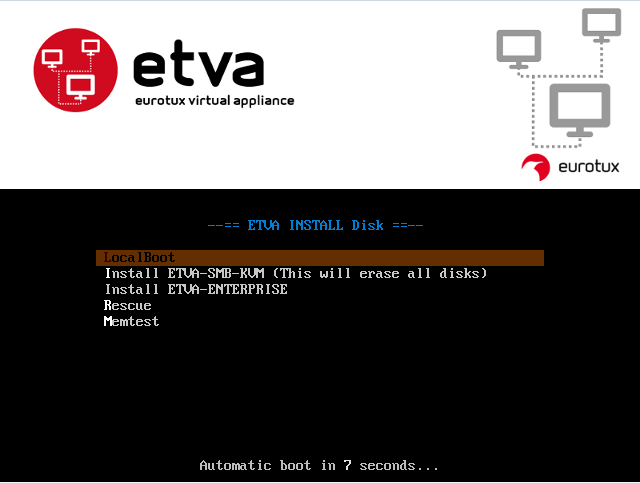
\includegraphics[scale=0.6]{screenshots/install_etva1.png}
	\caption{Menu de instalação da versão ETVA Standard}
	\label{fig:boot_install_screen_standard}
	\end{center}
\end{figure}

De seguida, seleccionando a opção \emph{"Install ETVA-SMB-KVM (This will erase all disks)"} iniciar-se-á o arranque da instalação conforme:

\begin{figure}[H]
	\begin{center}
	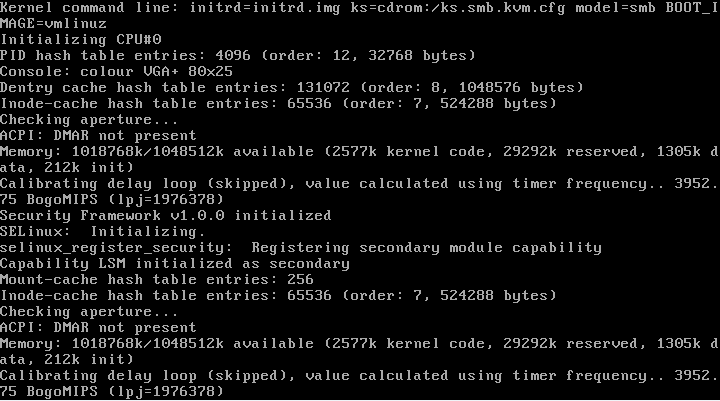
\includegraphics[scale=0.4]{screenshots/install_etva2.png}
    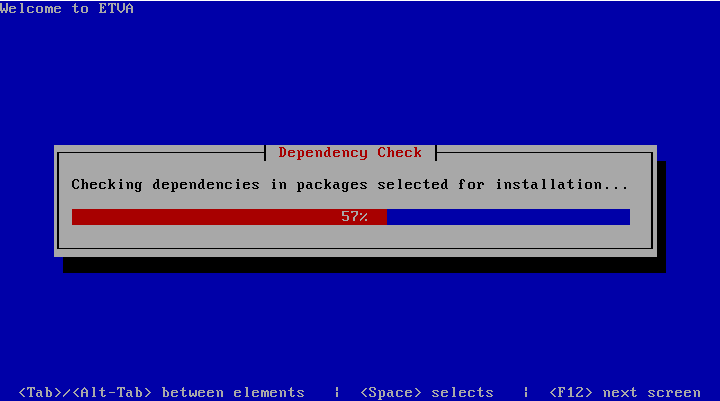
\includegraphics[scale=0.4]{screenshots/install_etva3.png}    
    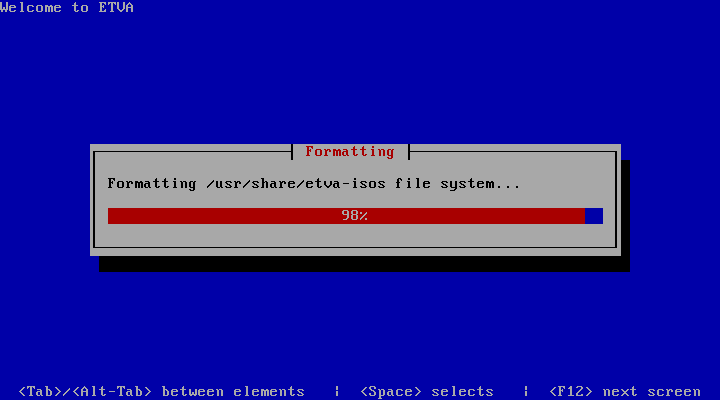
\includegraphics[scale=0.4]{screenshots/install_etva4.png}
    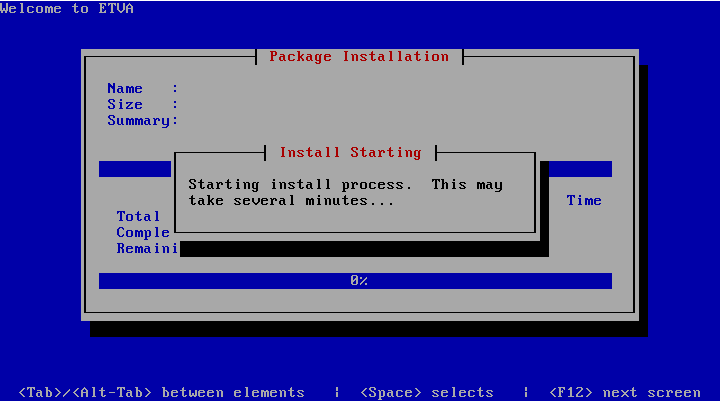
\includegraphics[scale=0.4]{screenshots/install_etva5.png}    
    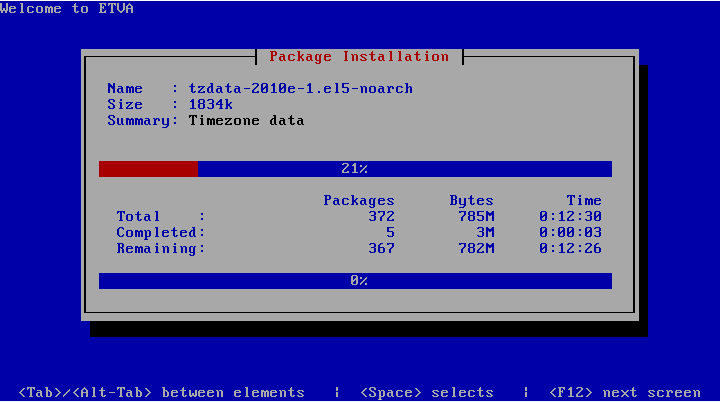
\includegraphics[scale=0.4]{screenshots/install_etva6.png}        
    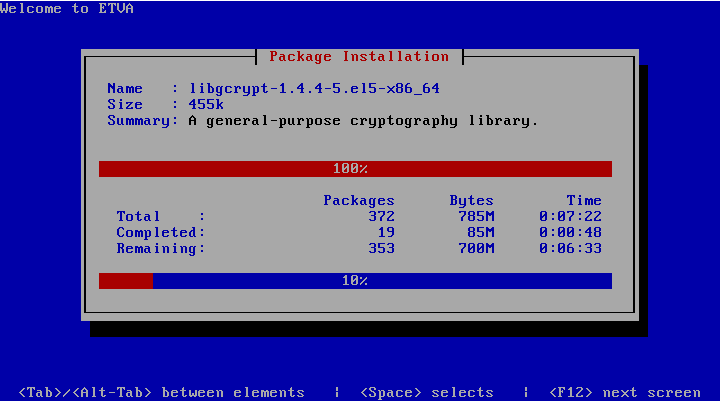
\includegraphics[scale=0.4]{screenshots/install_etva8.png}
    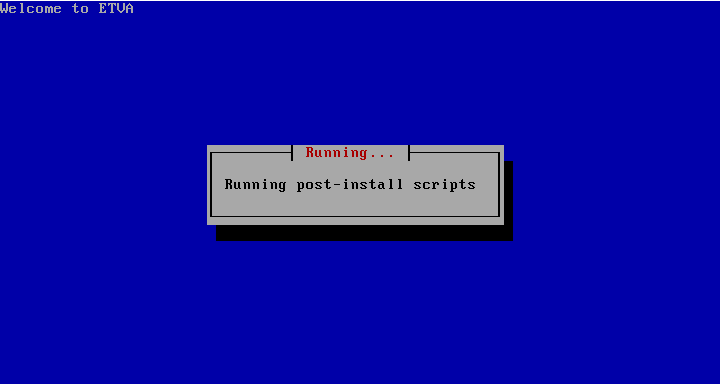
\includegraphics[scale=0.4]{screenshots/install_etva9.png}
    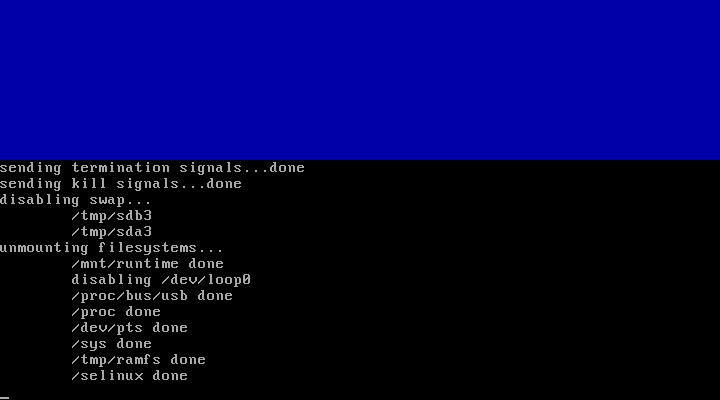
\includegraphics[scale=0.4]{screenshots/install_etva10.png}
\caption{Instalando a versão ETVA Standard}
	\label{fig:installation_standard}
	\end{center}
\end{figure}

Depois da instalação efectuada o arranque deverá ser efectuado a partir do disco rigido e deverá aparecer uma imagem como a seguinte:

\begin{figure}[H]
	\begin{center}
	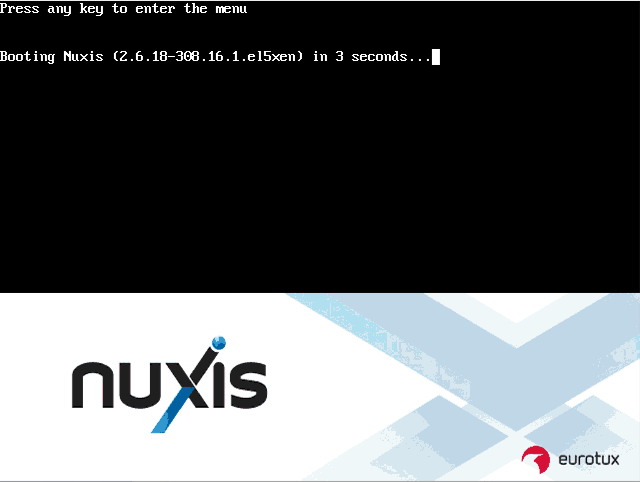
\includegraphics[scale=0.5]{screenshots/install_etva11.png}
	\caption{Menu de boot da versão ETVA Standard}
	\label{fig:boot_screen_standard}
	\end{center}
\end{figure}

No final da instalação deve-se ligar um cabo de rede do nosso PC de acesso à porta \emph{Management} conforme a figura \ref{fig:back_standard}.

\begin{figure}[H]
	\begin{center}
	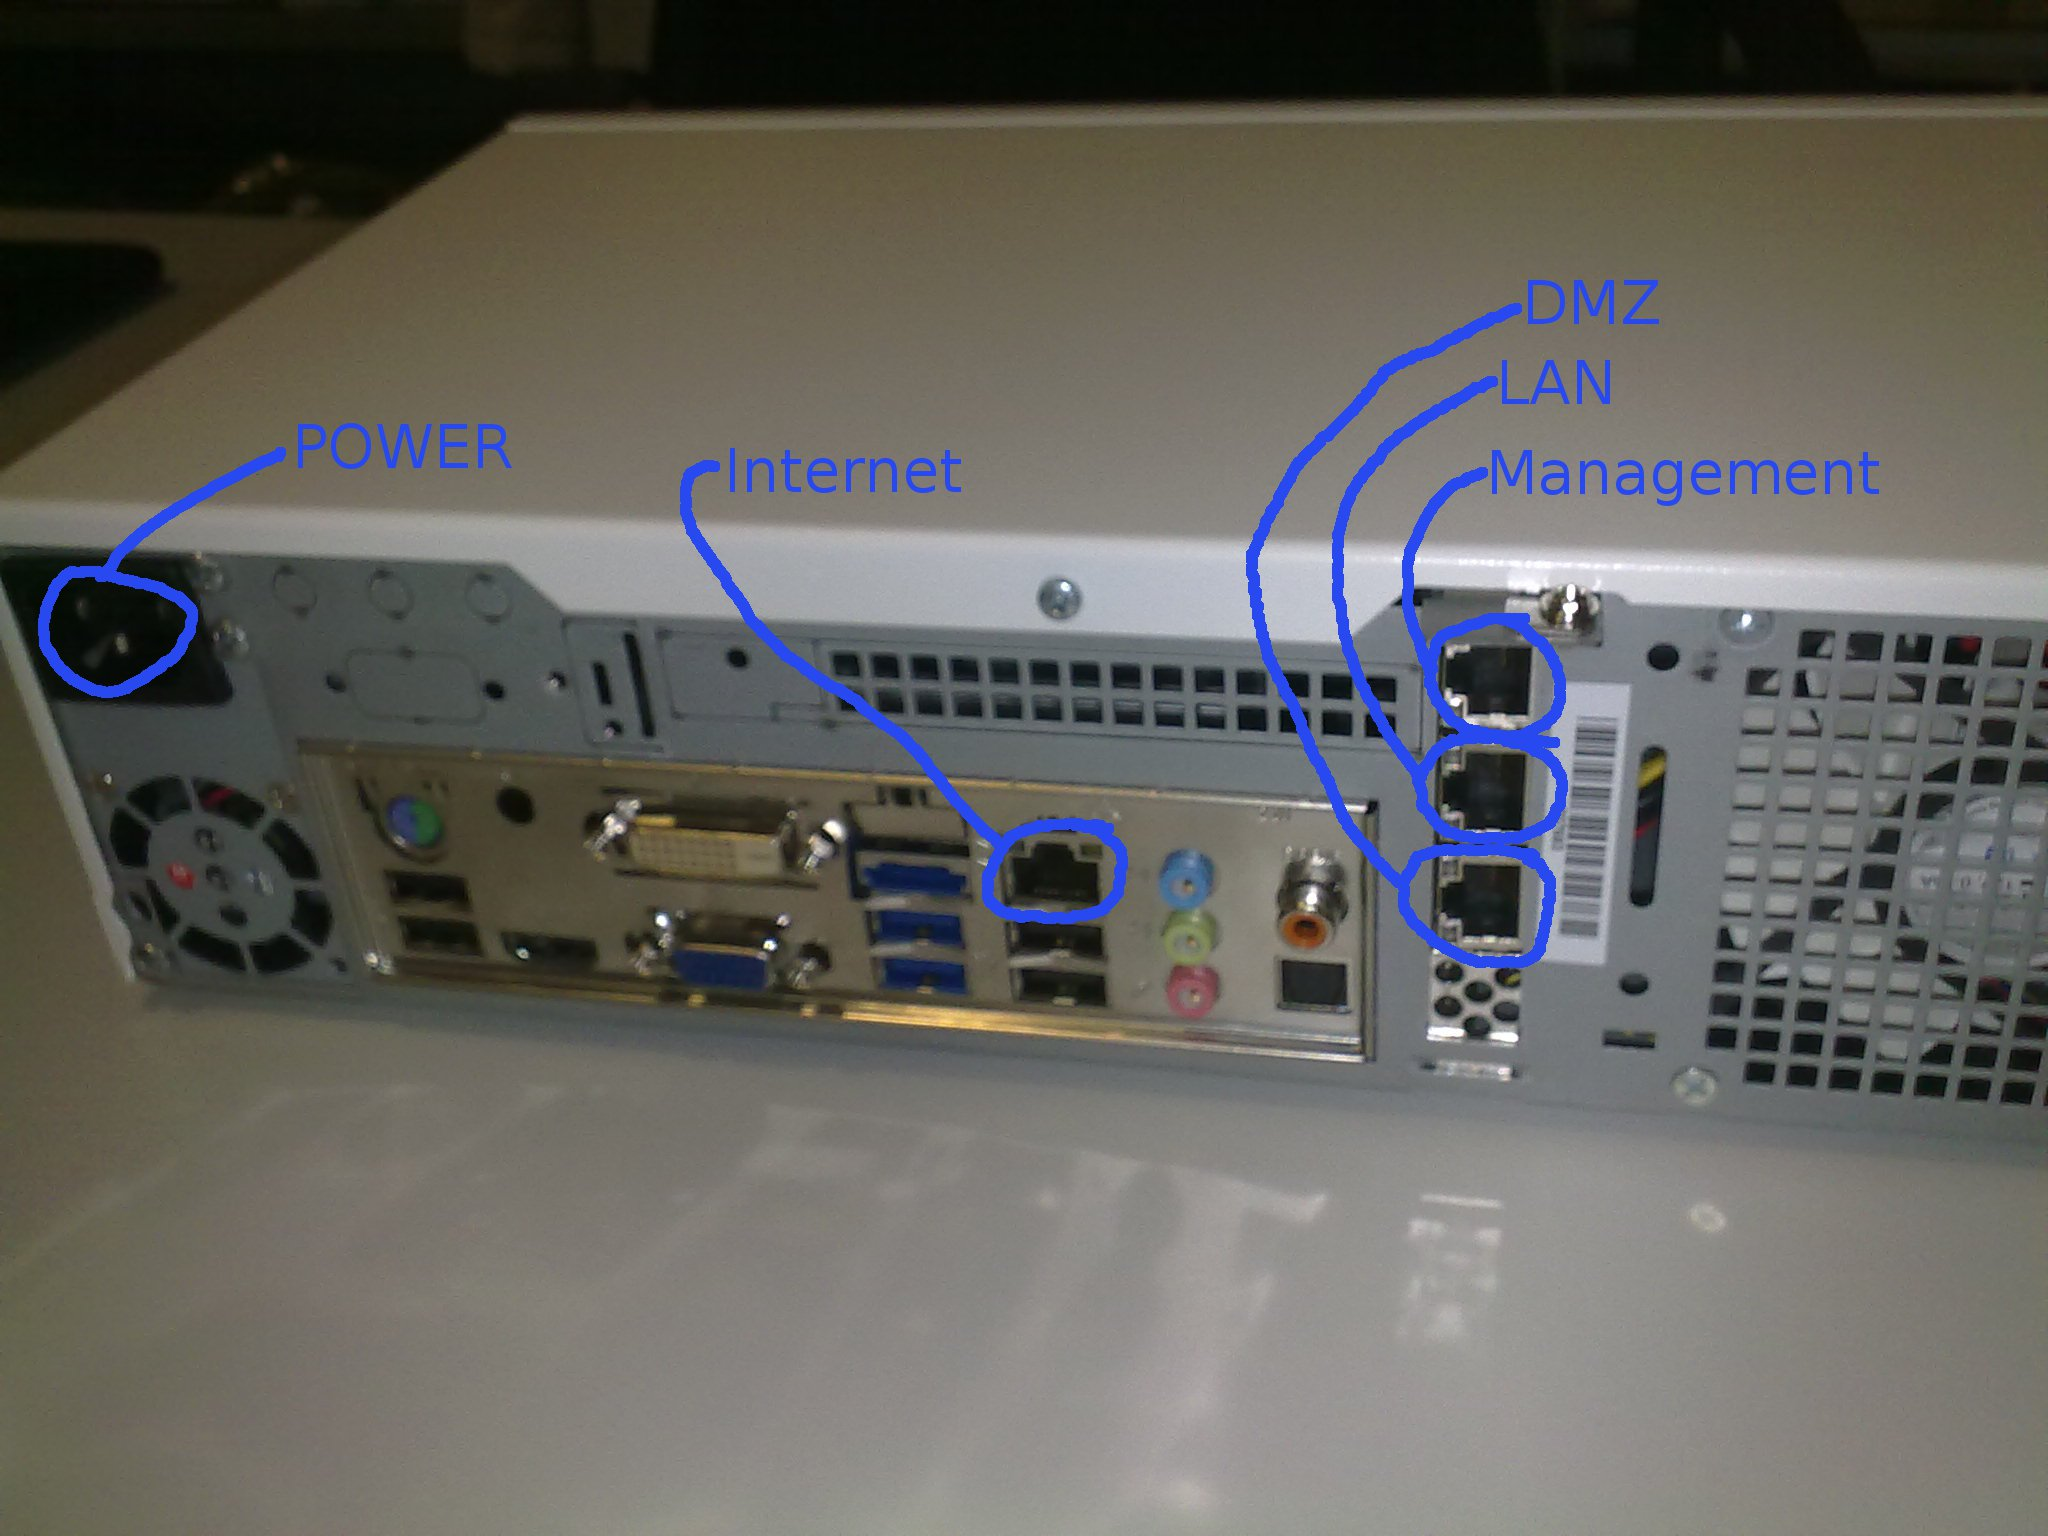
\includegraphics[scale=0.12]{screenshots/appliance_back_identifica.jpg}
	\caption{Identificação das portas a ligar na versão ETVA Standard}
	\label{fig:back_standard}
	\end{center}
\end{figure}

De seguida configura-se a placa de rede do nosso PC:

\begin{quote}
Endereço IP: 10.10.4.1\\
Máscara: 255.255.255.0
\end{quote}

Finalmente, abre-se o nosso browser e acede-se ao seguinte endereço:
\begin{quote}
http://10.10.4.254/
\end{quote}

\pagebreak
\chapter{\textsf{ETVA Central Management}}

\section{Estrutura da interface principal}
O layout principal é constituido por quatro áreas:

\begin{description}
	\item[Painel topo -] Possui menus de acesso a acções do sistema, tais como a administração de utilizadores, gestão de ISOs e visualização das mensagens do sistema.
	\item[Painel esquerdo (\emph{Nodes}) -] Lista as máquinas reais/servidores de virtualização - {\bf\emph{nodes}} e as máquinas virtuais associadas a cada \emph{node} - {\bf\emph{servidores}}. No nível imediatamente abaixo de \emph{Main} encontram-se os vários servidores de virtualização registados no CM. As funcionalidades permitidas num servidor de virtualização estão descritas na secção \ref{sec:node}. No nível abaixo de um \emph{node} encontram-se as máquinas virtuais do respectivo \emph{node}. As funcionalidades de uma máquina virtual encontram-se descritas na secção \ref{sec:server}. Ao clicar em cada item é carregada a informação correspondente no painel principal.
	\item[Painel principal -] Área onde é visualizada o conteúdo pretendido, consoante o contexto (item a visualizar).
	\item[Painel de informação (\emph{Painel de Informação}) -] Área de breve notificação acerca dos eventos despoletados pelo utilizador. Mensagens de erro e sucesso são aqui visualizadas.
\end{description}

\begin{figure}[H]
	\begin{center}
	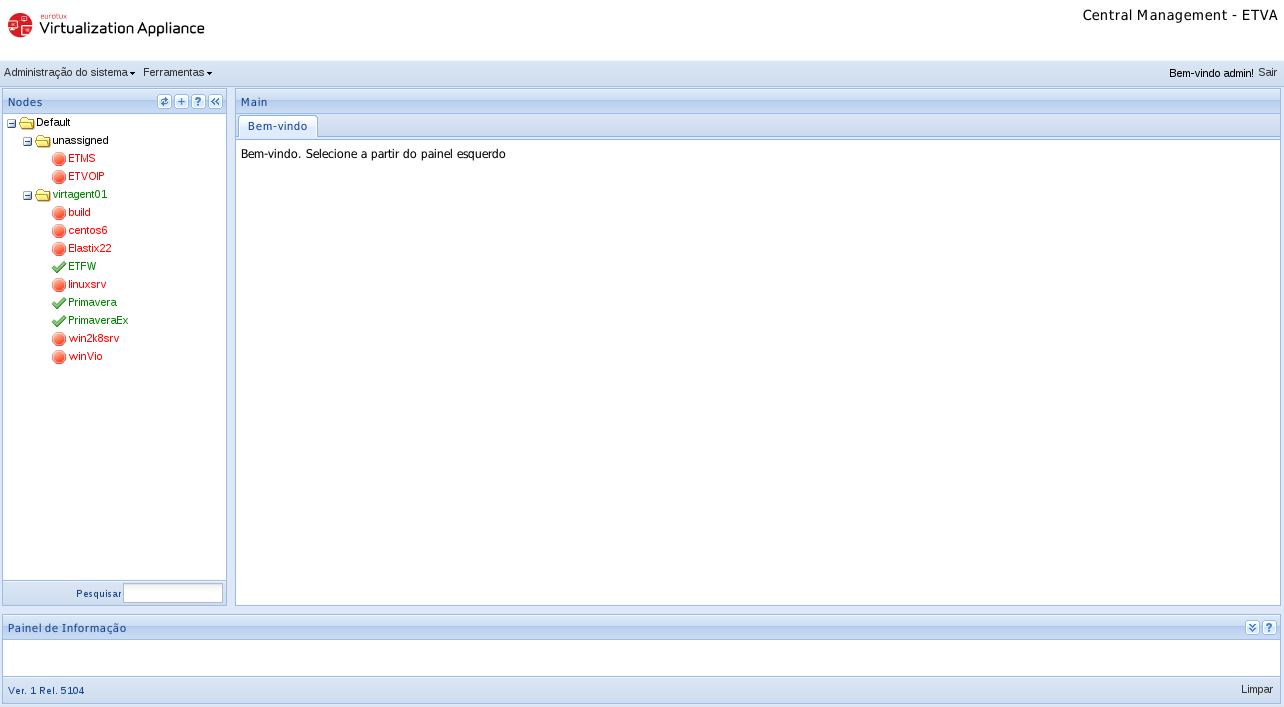
\includegraphics[scale=0.45]{screenshots/principal.png}
	\caption{Layout principal}
	\label{fig:principal}
	\end{center}
\end{figure}

\pagebreak


\section{Primeiro acesso}
\label{sec:first_access}
Após a instalação do CM pela primeira vez acede-se ao url do sistema disponível no endereço http://<ENDEREÇO IP>\footnote{Endereço especificado na {\bf \emph{Instalação}} (capítulo \ref{chp:installation}).}

\begin{figure}[H]
	\begin{center}
	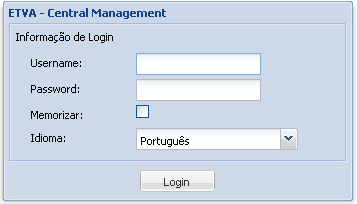
\includegraphics[scale=0.7]{screenshots/login.png}
	\caption{Página de autenticação}
	\label{fig:login}
	\end{center}
\end{figure}

A página de autenticação é disponibilizada e deverá ser introduzido o \emph{Username} e a respectiva \emph{Password}. Também é possível seleccionar o idioma do sistema\footnote{De momento apenas estão disponíveis os idiomas Português e Inglês}.

\begin{quote}
	{\large \bf Nota} \\*[-.8pc]
	\underline{\hspace{6in}} \\
	Ao instalar o CM pela primeira vez as credenciais de acesso são:
	\begin{description}
        	\item[Username:] admin
	        \item[Password:] admin
	\end{description}
	Por questões de segurança recomenda-se a alteração da password do sistema no primeiro acesso através do assistente de configuração inicial.

\end{quote}

No primeiro acesso ao \emph{Central Management} deverá surgir o \emph{Assistente de configuração inicial} que permite efectuar a configuração incial do sistema (ver secção \ref{sec:first_time_wizard}).

De seguida, e após a instalação e configuração de um agente virtualização num \emph{node}, este regista-se automáticamente no CM, passando o CM a dispor de mais funcionalidades.
No painel esquerdo, \emph{Nodes} (ver figura \ref{fig:principal}), surgirá o servidor de virtualização registado no CM e poderá então passar-se a efectuar a gestão desse \emph{node} conforme as opções descritas na secção \ref{sec:node}.

\pagebreak

\section{Main}

Neste painel é apresentada a vista geral do CM.
Podemos visualizar os servidores de virtualização e a informação da rede do CM (ver figura \ref{fig:main_nodes}).

\subsection{Nodes}

Em \emph{Nodes} é disponibilizada alguma informação acerca dos vários servidores de virtualização. Podemos ver o \emph{hypervisor} suportado pelas máquinas reais e, entre outras informações, o estado do agente de virtualização.
\begin{figure}[H]
	\begin{center}
	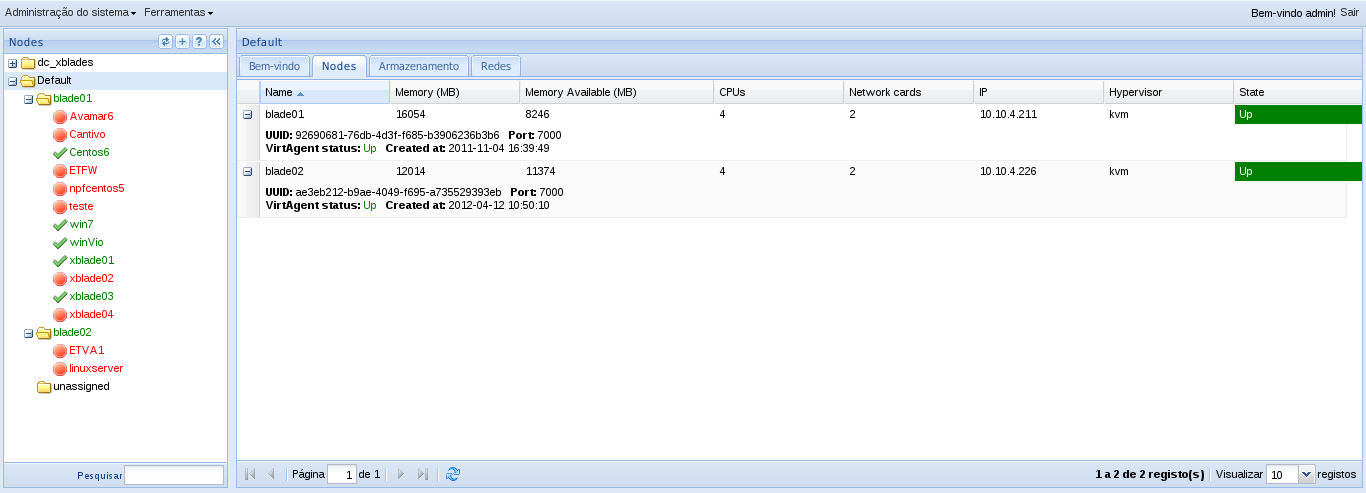
\includegraphics[scale=0.45]{screenshots/main_nodes.png}
	\caption{Vista dos nodes do Central Management}
	\label{fig:main_nodes}
	\end{center}
\end{figure}

\subsection{Redes}

Este painel permite efectuar as seguintes operações sobre o CM:

\begin{itemize}
	\item Administração das redes do sistema
	\item Gestão da pool de endereços MAC
	\item Gestão das interfaces de rede das máquinas virtuais 
\end{itemize}

\begin{figure}[H]
	\begin{center}
	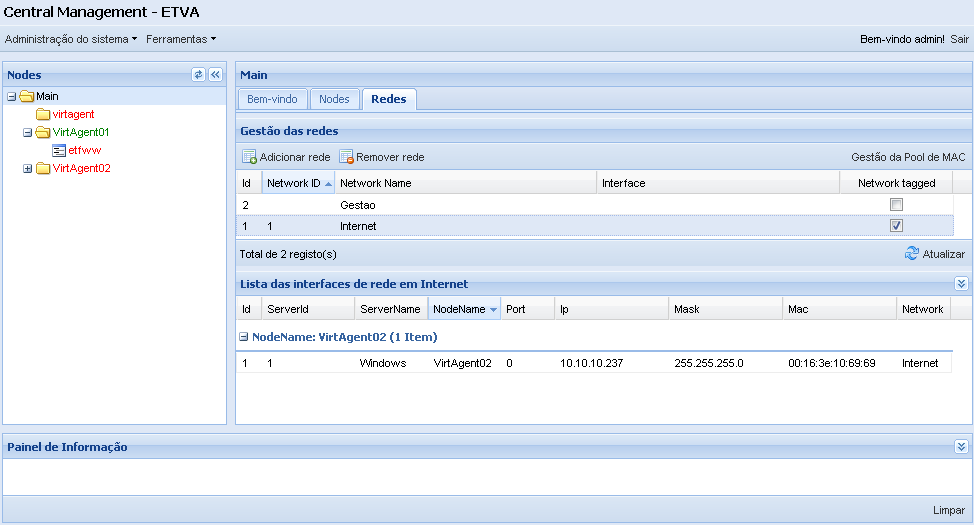
\includegraphics[scale=0.45]{screenshots/main_networks.png}
	\caption{Vista das redes do sistema  e das interfaces de rede}
	\label{fig:main_networks}
	\end{center}
\end{figure}

É possível também filtrar as interface de rede numa determinada rede clicando sobre a rede pretendida conforme a figura \ref{fig:main_networks}.
Na figura \ref{fig:main_networks} as interfaces de rede listadas são as que estão associadas à rede \emph{Internet}

\subsubsection{Administração das redes}

Para criar uma rede clica-se em \emph{Adicionar rede}.
A informação da rede consiste no seu nome e ID\footnote{Caso a rede/vlan seja \emph{tagged} o campo \emph{ID da rede} refere-se à \emph{VLAN ID}} (ver figura \ref{fig:network_create}).

Para remover uma rede selecciona-se a rede pretendida e clica-se em \emph{Remover rede}.

\begin{quote}
	{\large \bf Nota} \\*[-.8pc]
	\underline{\hspace{6in}} \\
	As operações de adicionar/remover rede só estão disponíveis na versão \emph{ETVA Enterprise}.
\end{quote}


\begin{figure}[H]
	\begin{center}
	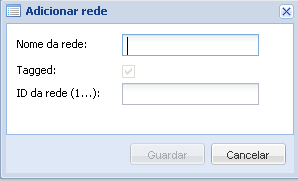
\includegraphics[scale=0.5]{screenshots/network_create.png}
	\caption{Janela de criação de uma rede}
	\label{fig:network_create}
	\end{center}
\end{figure}

A rede adicionada/removida é propagada a todos os \emph{nodes} do CM.


\subsubsection{Gestão da pool de endereços MAC}
\label{sec:mac_pool}

Em \emph{Gestão da Pool de MAC} (ver figura \ref{fig:main_networks}), é possivel criar a pool de endereços MAC.
Para além de adicionar MACs à pool, pode-se visualizar as redes associadas e os MACs ainda disponíveis da pool.

\begin{figure}[H]
	\begin{center}
	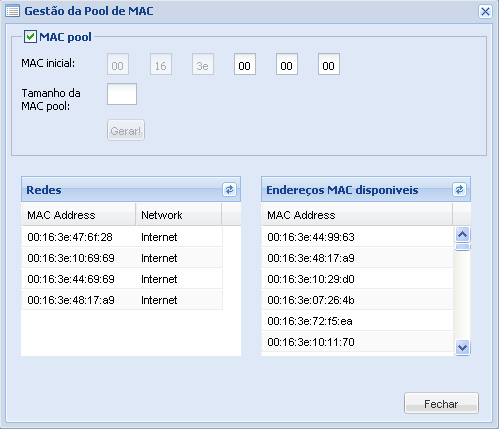
\includegraphics[scale=0.5]{screenshots/networks_macpool.png}
	\caption{Janela de criação da pool de MACs}
	\label{fig:networks_macpool}
	\end{center}
\end{figure}


\subsubsection{Gestão das interfaces de rede das máquinas virtuais}
Seleccionando um registo da tabela de interfaces e acedendo ao sub-menu de contexto, é possível remover a interface de rede associada a esse registo - \emph{Remover interface de rede}, ou alterar as interfaces de rede da máquina virtual associada ao registo seleccionado - \emph{Gestão das interfaces de rede}.

\begin{figure}[H]
	\begin{center}
	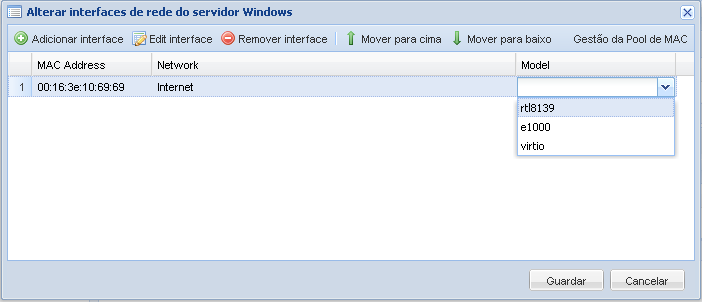
\includegraphics[scale=0.5]{screenshots/nics.png}
	\caption{Janela de gestão das interfaces de rede de uma máquina virtual}
	\label{fig:nics}
	\end{center}
\end{figure}

Na gestão de interfaces de uma máquina, dependendo do tipo de máquina virtual é possível seleccionar os drivers das placas de rede.\footnote{Esta opção está disponível para máquinas em HVM ou KVM.Os drivers disponíveis são: e1000, rtl8139 e virtio}

% PAINEL NODE

\section{Servidor de virtualização}
\label{sec:node}

No painel \emph{Nodes} é possivel seleccionar um \emph{node}(servidor de virtualização), e efectuar as seguintes operações:
\begin{itemize}
    \item Visualizar informação do \emph{node} (ver secção \ref{sec:nodeinfo})
    \item Gestão de máquinas virtuais (ver secção \ref{sec:servers})
    \item Gestão do armazenamento do node (ver secção \ref{sec:storage})
\end{itemize}

Para além das operações mencionadas acima, é possível aceder ao sub-menu de contexto de um \emph{node} que permite operações de:
\begin{itemize}
    \item Carregar node
    \item Opções de conectividade\footnote{Disponível apenas na versão \emph{ETVA Enterprise}}
    \item Alterar keymap
    \item Estado do node
\end{itemize}

Em \emph{Opções de conectividade}, é possível editar a configuração da interface \emph{Management} ao qual se encontra ligado o agente de virtualização.
\begin{figure}[H]
	\begin{center}
	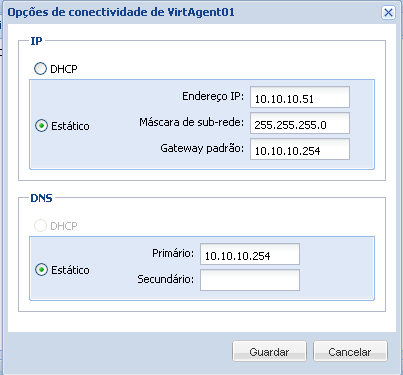
\includegraphics[scale=0.5]{screenshots/node_conn.png}
	\caption{Configuração da conectividade do agente \emph{VirtAgent01}}
	\label{fig:node_conn}
	\end{center}
\end{figure}

Em \emph{Alterar keymap}, consoante o item seleccionado, servidor de virtualização ou máquina virtual, é possível definir o keymap padrão usado pelo VNC, ou o keymap específico a uma determinada máquina virtual respectivamente.

Em \emph{Estado do node}, é possível enviar ao servidor de virtualização um pedido de verificação do estado da conectividade do agente.

\subsection{Informação do node}
\label{sec:nodeinfo}
Em \emph{Informação do node} é disponibilizada a informação acerca do servidor de virtualização. Podemos ver o \emph{hypervisor} suportado pela máquina real e, entre outras informações, o estado do agente de virtualização.

\begin{figure}[H]
	\begin{center}
	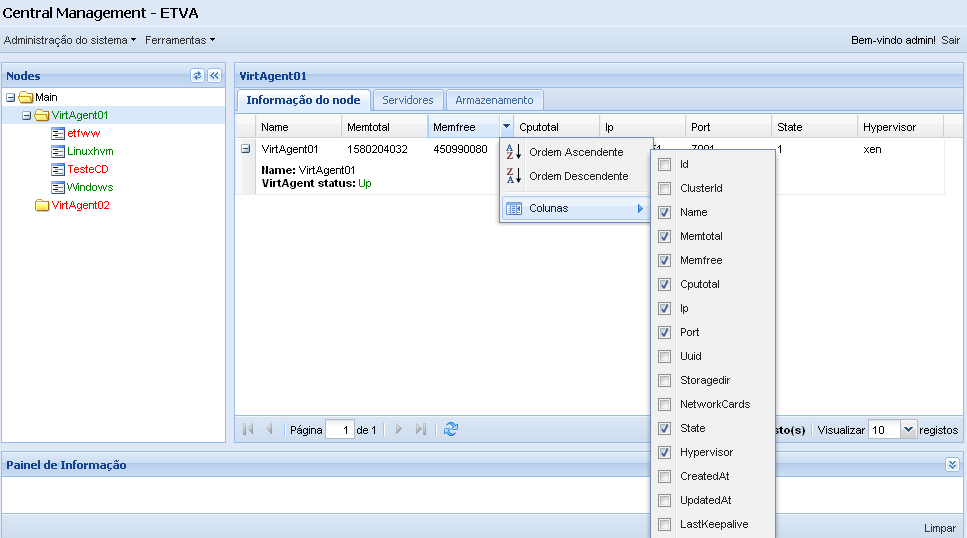
\includegraphics[scale=0.45]{screenshots/node_info.png}
	\caption{Informação do node \emph{VirtAgent01}}
	\label{fig:node_info}
	\end{center}
\end{figure}

\subsection{Servidores}
\label{sec:servers}
Em \emph{Servidores} é disponibilizada a informação acerca das máquinas virtuais existente no servidor de virtualização. Para além de visualizar informação, este painel permite efectuar as seguintes operações:
\begin{itemize}
	\item Adicionar máquina virtual
    \item Editar máquina virtual
	\item Remover maquina virtual
	\item Abrir máquina virtual numa consola VNC
	\item Iniciar/parar máquina virtual
    \item Migrar máquina virtual
\end{itemize}
\begin{figure}[H]
	\begin{center}
	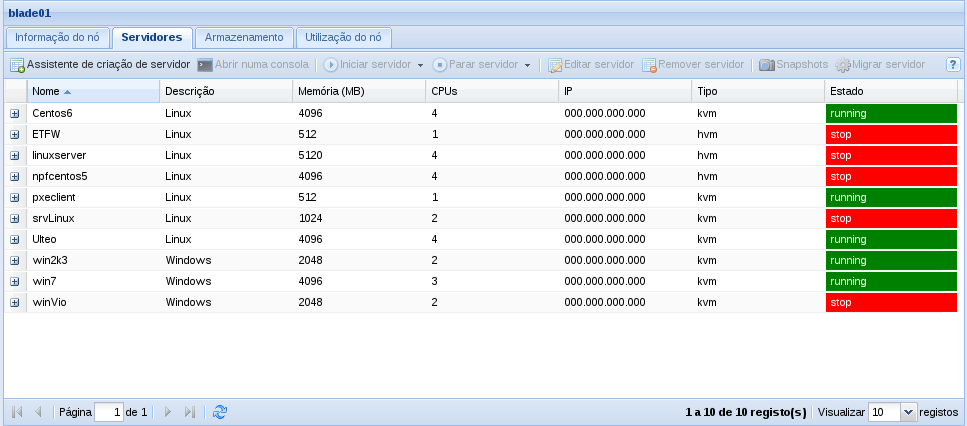
\includegraphics[scale=0.45]{screenshots/node_servers.png}
	\caption{Lista das máquinas virtuais do node \emph{VirtAgent01}}
	\label{fig:node_servers}
	\end{center}
\end{figure}

\subsubsection{Adicionar máquina virtual}
\label{sec:add_server}

Para adicionar uma nova máquina virtual utiliza-se o botão \emph{Assistente de criação de servidor}.
\begin{quote}
	{\large \bf Nota} \\*[-.8pc]
	\underline{\hspace{6in}} \\
	As opções deste painel só se encontram activas se o agente de virtualização estiver a correr no \emph{node} (máquina real) e este conseguir estabelecer comunicação com o CM.
\end{quote}
 

\begin{figure}[H]
	\begin{center}
	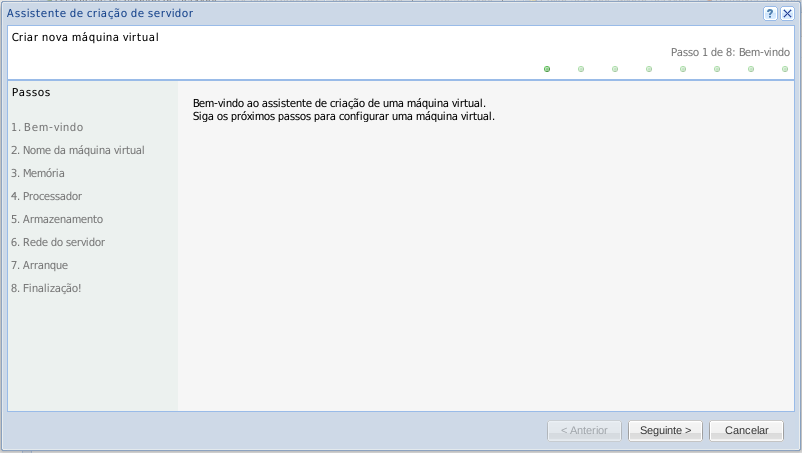
\includegraphics[scale=0.5]{screenshots/server_createwiz.png}
	\caption{Assistente de criação de servidor - Bem-vindo}
	\label{fig:server_createwiz}
	\end{center}
\end{figure}
Este assistente é constituido pelas seguintes etapas:
\begin{description}
	\item[Nome da máquina virtual:] Nesta etapa define-se o nome da máquina virtual e o tipo de sistema operativo. As opções do sistema operativo variam consoante a especificação do node:
		\begin{itemize}
			\item com XEN e suporte a virtualização por hardware:
			\begin{itemize}
				\item Linux PV
				\item Linux HVM
				\item Windows
			\end{itemize}
 			\item com XEN sem suporte de virtualização por hardware:
			\begin{itemize}
				\item Linux PV
			\end{itemize}
 			\item com KVM
			\begin{itemize}
				\item Linux
				\item Windows
			\end{itemize}
		\end{itemize}
	
		\begin{figure}[H]
        		\begin{center}
		        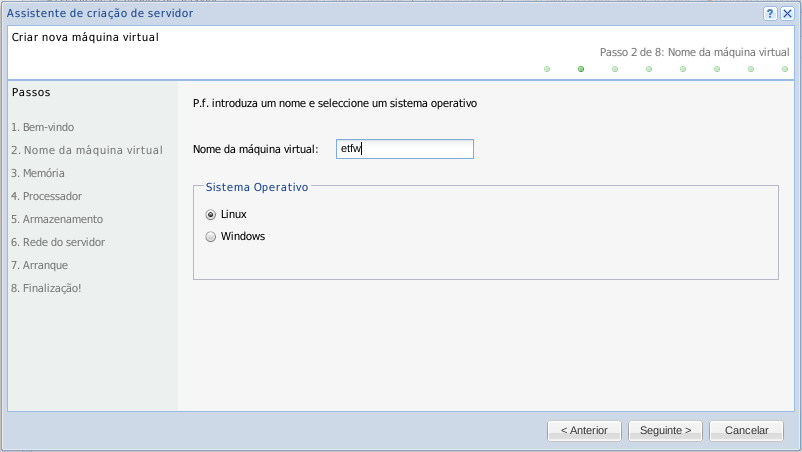
\includegraphics[scale=0.5]{screenshots/server_createwiz_name.png}
        		\caption{Assistente de criação de servidor - Nome da máquina virtual}
	        	\label{fig:server_createwiz_name}
	        	\end{center}
		\end{figure}
 
	\item[Memória:] Especificação da memória a ser usada pela máquina.
		\begin{figure}[H]
        		\begin{center}
		        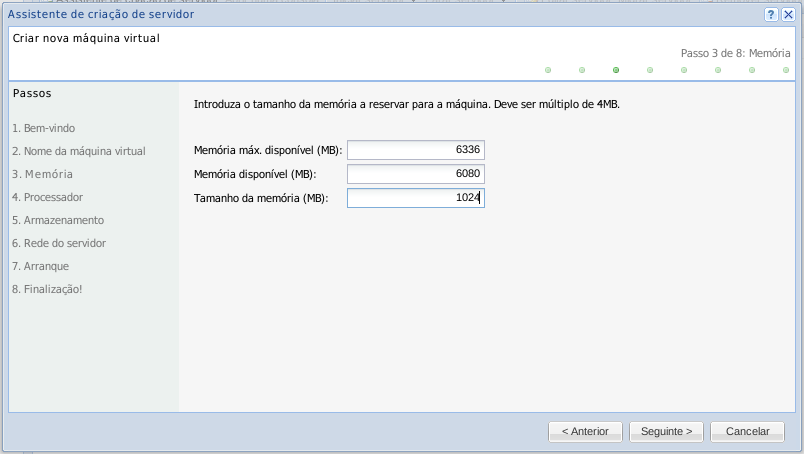
\includegraphics[scale=0.5]{screenshots/server_createwiz_memory.png}
        		\caption{Assistente de criação de servidor - Memória}
	        	\label{fig:server_createwiz_memory}
	        	\end{center}
		\end{figure}

	\item[Processador:] Nesta etapa define-se o número de processadores a usar.
		\begin{figure}[H]
        		\begin{center}
		        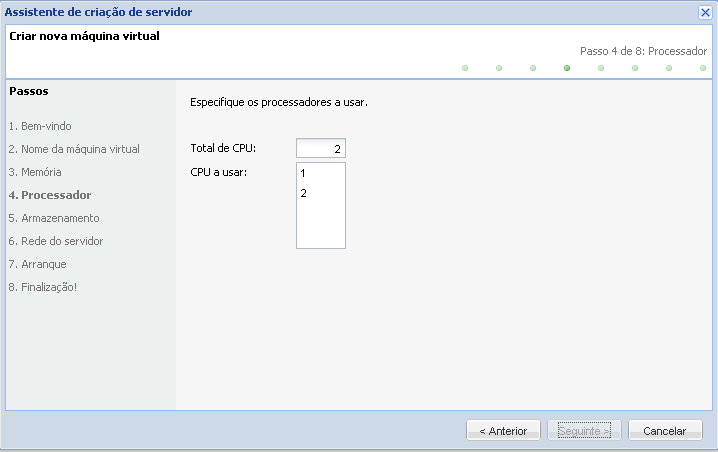
\includegraphics[scale=0.5]{screenshots/server_createwiz_processor.png}
        		\caption{Assistente de criação de servidor - Processador}
		        \label{fig:server_createwiz_processor}
	        	\end{center}
		\end{figure}

	\item[Armazenamento:] Define o disco de arranque da máquina virtual. Pode ser uma das três opções:
\begin{itemize}
	\item usar um logical volume/ficheiro já existente - \emph{Logical volume existente}
	\item criar um novo logical volume/ficheiro (para criar um ficheiro através desta opção tem que se seleccionar o volume group \emph{\_\_DISK\_\_}\footnote{Ver secção \ref{sec:storage}}) - \emph{Novo logical volume}
	\item  ou caso pretenda criar um ficheiro usar a opção \emph{Novo ficheiro} que para tal necessita apenas do nome e tamanho.
\end{itemize}

        \begin{figure}[H]
        		\begin{center}
	        	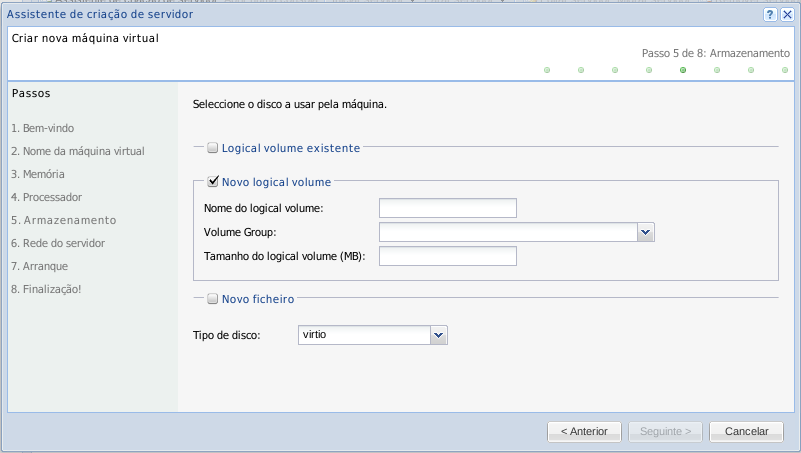
\includegraphics[scale=0.5]{screenshots/server_createwiz_storage.png}
	        	\caption{Assistente de criação de servidor - Armazenamento}
		        \label{fig:server_createwiz_storage}
        		\end{center}
		\end{figure}

		\begin{quote}
			{\large \bf Nota} \\*[-.8pc]
			\underline{\hspace{6in}} \\
			Se o \emph{node} não suportar \emph{physical volumes} a opção \emph{Logical volume existente} será desabilitada, uma vez que não é possivel criar \emph{logical volumes}, mas sim apenas ficheiros.
		\end{quote}		
        
        
        \item[Rede do servidor:] Especificação das interfaces de rede existentes no servidor. Caso não existam endereços MAC disponíveis é possível criar através de \emph{Gestão da Pool de MAC}. Igualmente para as redes é possível criar nesta etapa através de \emph{Adicionar rede}.
		\begin{figure}[H]
        		\begin{center}
	        	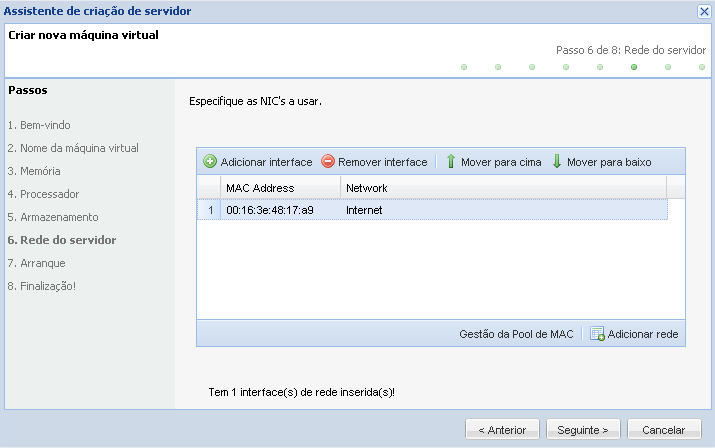
\includegraphics[scale=0.5]{screenshots/server_createwiz_hostnet.png}
	        	\caption{Assistente de criação de servidor - Rede do servidor}
		        \label{fig:server_createwiz_hostnet}
        		\end{center}
		\end{figure}

        \item[Arranque:] Especificação de parâmetros de arranque da máquina virtual. As opções nesta etapa variam consoante o tipo de sistema definido na etapa \emph{Nome da máquina virtual}:
		\label{sec:add_server_boot}
        \begin{itemize}
			\item \emph{Linux PV}
				\begin{itemize}
					\item Instalação via rede. Url do kernel a carregar.
				\end{itemize}
			\item Outros
				\begin{itemize}
					\item Boot de rede (PXE)
					\item CD-ROM (ISO)
				\end{itemize}
		\end{itemize}
        A figura \ref{fig:server_createwiz_startup} refere-se às opções de uma máquina virtual em \emph{Linux PV}.

		\begin{figure}[H]
			\begin{center}
			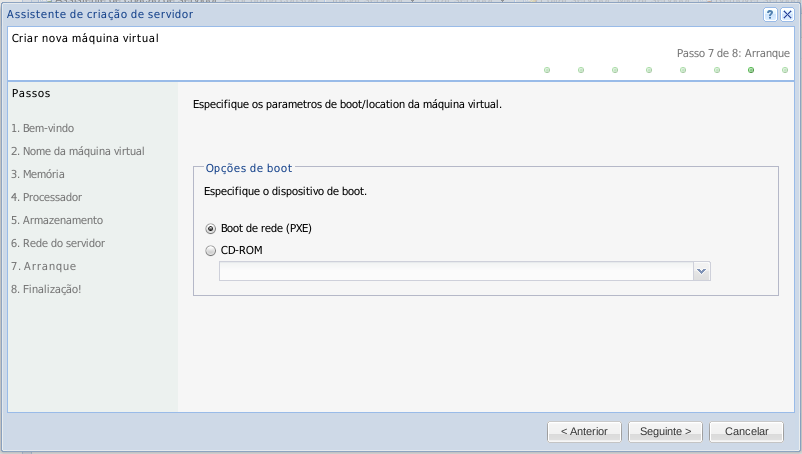
\includegraphics[scale=0.5]{screenshots/server_createwiz_startup.png}
			\caption{Assistente de criação de servidor - Arranque}
			\label{fig:server_createwiz_startup}
			\end{center}
		\end{figure}

	\item[Finalização!] Etapa final do assistente. Após confirmação da criação do servidor, os dados recolhidos nas etapas anteriores são processados e enviados ao servidor de virtualização. Posteriormente no painel \emph{Servidores} poderá ser iniciada a máquina através da opção \emph{Iniciar servidor}.
		\begin{figure}[H]
			\begin{center}
			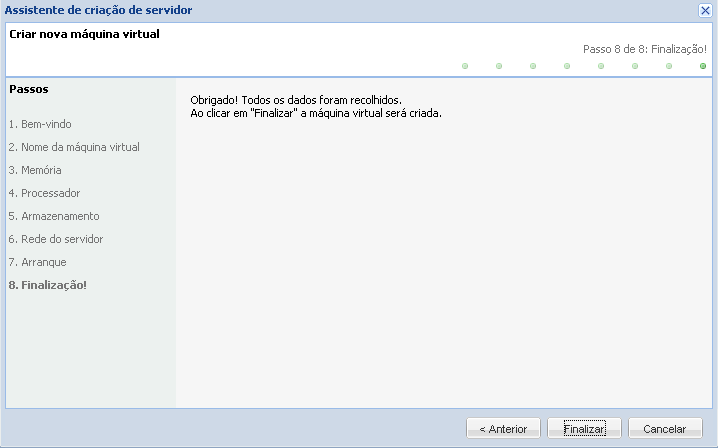
\includegraphics[scale=0.5]{screenshots/server_createwiz_finish.png}
			\caption{Assistente de criação de servidor - Finalização!}
			\label{fig:server_createwiz_finish}
			\end{center}
		\end{figure}

\end{description}

\subsubsection{Editar máquina virtual}
\label{sec:edit_server}
Para editar um servidor, selecciona-se a máquina pretendida e clica-se em \emph{Editar servidor}.

    \begin{quote}
        {\large \bf Nota} \\*[-.8pc]
        \underline{\hspace{6in}} \\
        Se a máquina virtual for do tipo PV, é possivel fazer alterações com a máquina a correr, caso contrário a opção encontra-se desabilitada, sendo necessário que a máquina não se encontre activa para poder efectuar alterações.
    \end{quote}

A edição de uma máquina virtual permite a configuração de:
\begin{description}
	\item[Opções gerais:] Neste painel é permitido alterar o nome, memória, opções do keymap e parâmetros de boot da máquina.
        Os parâmetros de boot variam consoante o tipo da máquina virtual (ver secção \ref{sec:add_server_boot}).
		\begin{figure}[H]
        		\begin{center}
		        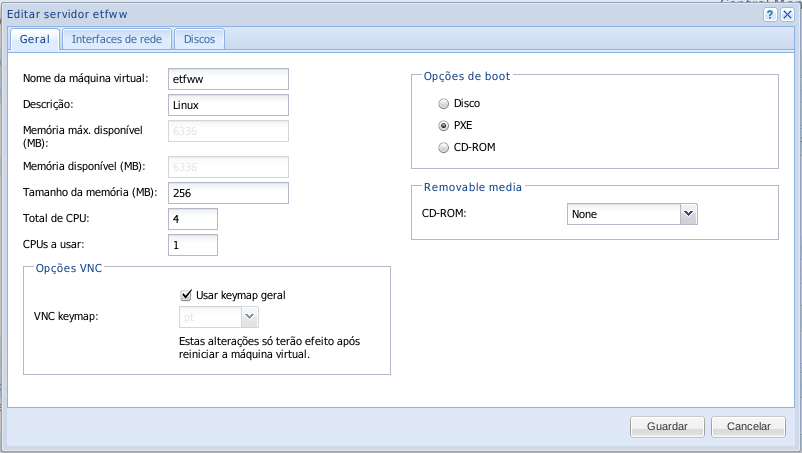
\includegraphics[scale=0.5]{screenshots/server_edit_general.png}
        		\caption{Edição de um servidor - Opções gerais}
	        	\label{fig:server_edit_general}
	        	\end{center}
		\end{figure}

	\item[Interfaces de rede:] Adicionar/remover interfaces. É possível alterar o tipo de driver a usar se aplicável\footnote{Só é possível especificar o driver a usar se a máquina virtual for HVM ou KVM}.
		\begin{figure}[H]
        		\begin{center}
		        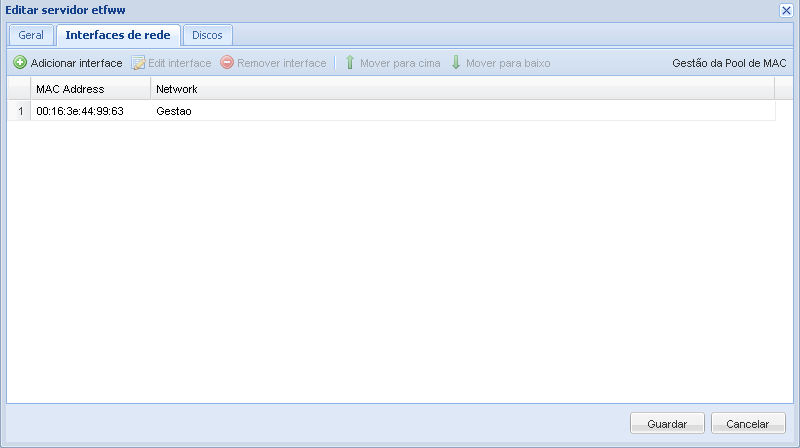
\includegraphics[scale=0.5]{screenshots/server_edit_interfaces.png}
        		\caption{Edição de um servidor - Interfaces de rede}
	        	\label{fig:server_edit_interfaces}
	        	\end{center}
		\end{figure}

	\item[Discos:] Adicionar/remover discos da máquina. A máquina virtual tem que ter pelo menos um disco associado.
                    Para adicionar/remover discos selecciona-se o disco pretendido e recorre-se ao \emph{drag-n-drop} entre as tabelas.
                    
                \begin{quote}
                    {\large \bf Nota} \\*[-.8pc]
                    \underline{\hspace{6in}} \\
                    O disco de boot da máquina é o disco que se encontra na primeira posição da tabela.
                \end{quote}
                    
		\begin{figure}[H]
        		\begin{center}
		        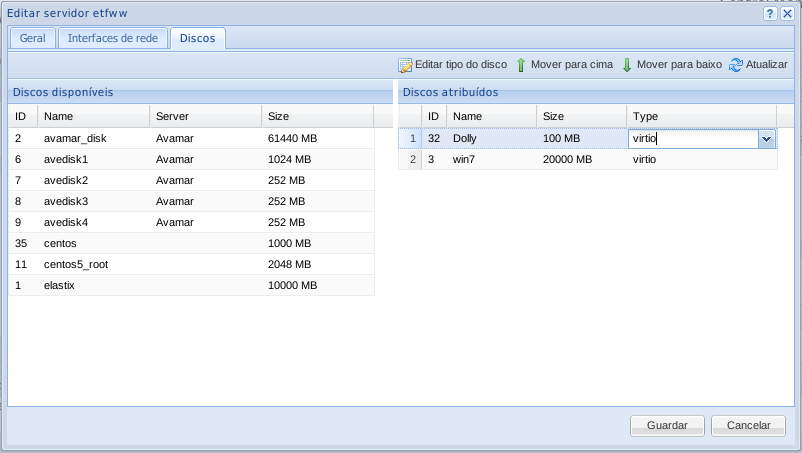
\includegraphics[scale=0.5]{screenshots/server_edit_disks.png}
        		\caption{Edição de um servidor - Discos}
		        \label{fig:server_edit_disks}
	        	\end{center}
		\end{figure}

\end{description}



\subsubsection{Remover máquina virtual}
\label{sec:remove_server}
Para remover um servidor, selecciona-se a máquina a remover e clica-se em \emph{Remover servidor}.

A opção \emph{Manter disco} permite manter o disco associado à máquina aquando da sua criação, caso contrário será também removido.
		
\begin{figure}[H]
	\begin{center}
	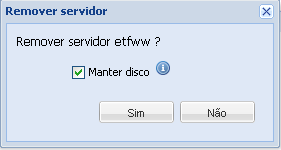
\includegraphics[scale=0.5]{screenshots/server_remove.png}
	\caption{Janela de remoção de um servidor}
	\label{fig:server_remove}
	\end{center}
\end{figure}

\subsubsection{Abrir máquina virtual numa consola VNC}
\label{sec:open_vnc}

Seleccionando um servidor e de seguida clicando em \emph{Abrir numa consola} é possível estabelecer uma ligação VNC com a máquina, desde que esta esteja a correr.

\begin{quote}
	{\large \bf Nota} \\*[-.8pc]
	\underline{\hspace{6in}} \\
	Caso o teclado esteja desconfigurado é possível alterar o \emph{keymap} do VNC através da opção \emph{Alterar keymap} no sub-menu de contexto do painel \emph{Nodes}.
    O \emph{keymap} pode ser definido quer ao nível de cada servidor, ou definir um \emph{keymap} de uso geral, o qual será usado por omissão na criação de novas máquinas virtuais.
\end{quote}

\subsubsection{Iniciar/parar máquina virtual}
\label{sec:start_server}

No arranque da máquina virtual é possível escolher um dos seguintes parâmetro de boot:
\begin{description}
	\item[Disco:] Arranque pelo disco associado ao servidor.
    \item[PXE:] Arranque por PXE\footnote{Só disponível caso o tipo da máquina virtual não seja \emph{Linux PV}\label{foot:notpv}}.
    \item[Location URL:] Arranque pelo url definido em Location\footnote{Só disponível caso o tipo da máquina virtual seja \emph{Linux PV}}.
	\item[CD-ROM:] Arranque pela imagem montada no CD-ROM\footref{foot:notpv}.
    	 
\end{description}

\begin{figure}[H]
	\begin{center}
	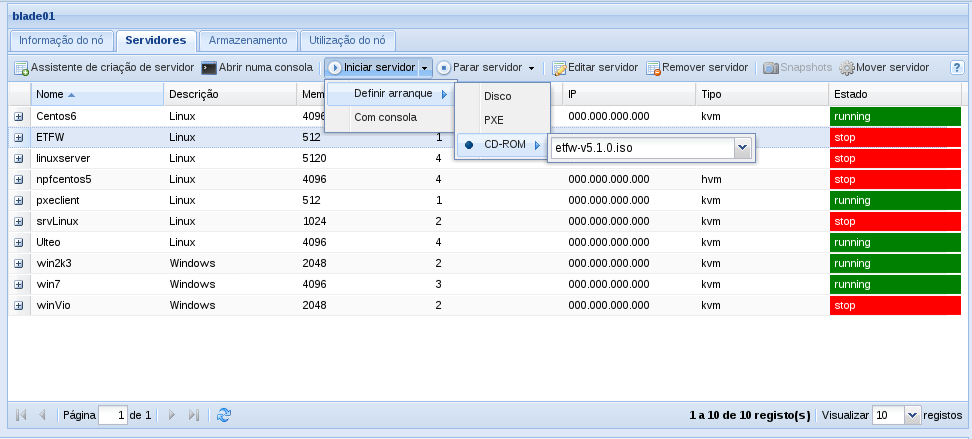
\includegraphics[scale=0.45]{screenshots/server_start.png}
	\caption{Parâmetros de arranque de uma máquina virtual}
	\label{fig:server_start}
	\end{center}
\end{figure}


\subsubsection{Migrar máquina virtual}
\label{sec:migrate_server}

Seleccionando um servidor e de seguida clicando em \emph{Migrar servidor} é possível migrar uma máquina de um \emph{node} para outro desde que partilhem o mesmo armazenamento.
A migração de uma máquina virtual é efectuada no modo \emph{offline}.

\begin{figure}[H]
	\begin{center}
	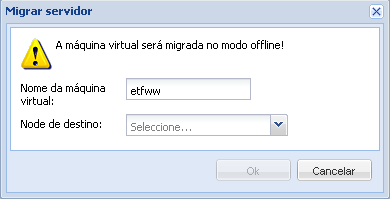
\includegraphics[scale=0.5]{screenshots/server_migrate.png}
	\caption{Migração de uma máquina virtual}
	\label{fig:server_migrate}
	\end{center}
\end{figure}

\begin{quote}
	{\large \bf Nota} \\*[-.8pc]
	\underline{\hspace{6in}} \\
	Esta opção só está disponível no modelo \emph{ETVA Enterprise}.
\end{quote}


\subsection{Armazenamento}
\label{sec:storage}

Em \emph{Armazenamento} encontra-se a informação relativa aos volumes existentes no \emph{node}.
Este painel encontra-se divido em três secções:

\begin{description}
	\item[Devices -] Informação relativa aos \emph{physical volumes}\footnote{Um \emph{physical volume} é um dispositivo fisico, como por exemplo um disco} e seu estado. Permite fazer a administração de \emph{physical volumes} do \emph{node}.
	\item[Volume Groups -] Lista os \emph{volumes groups}\footnote{Um \emph{volume group} consiste na agregação de diversos \emph{physical volumes} num único volume virtual} existentes no node e seus \emph{physical volumes} associados. Permite fazer operações de administração de \emph{volume groups}.
	\item[Logical Volumes -] Apresenta a informação dos \emph{logical volumes}\footnote{Um \emph{logical volume} é uma "fatia" de um \emph{volume group}. É usado como sendo uma partição do sistema} do \emph{node}. Área de administração dos \emph{logical volumes}.
\end{description}


\begin{quote}
	{\large \bf Nota} \\*[-.8pc]
	\underline{\hspace{6in}} \\
	Existe um \emph{volume group} especial, \_\_DISK\_\_, utilizado no manuseamento de ficheiros. Esta etiqueta serve para, aquando da criação de um \emph{logical volume}, indicar que o disco a ser usado não é de facto um \emph{logical volume} mas sim um ficheiro.
\end{quote}


\begin{figure}[H]
	\begin{center}
	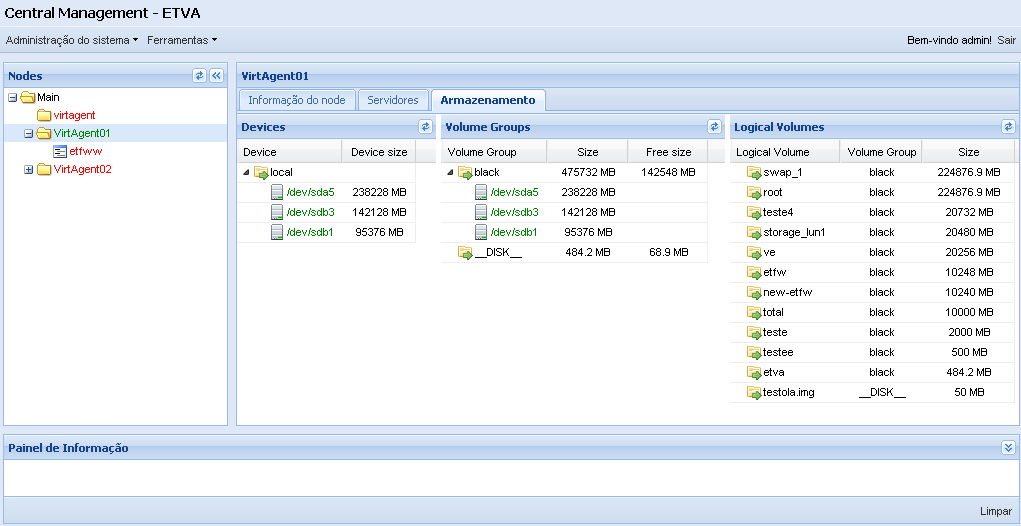
\includegraphics[scale=0.45]{screenshots/node_storage.png}
	\caption{Informação do armazenamento de um \emph{node}}
	\label{fig:inicial}
	\end{center}
\end{figure}

% ADMINISTRAÇÃO PHYSICAL VOLUMES

\subsubsection{Administração de Physical Volumes}
A administração de \emph{physical volumes} consiste nas seguintes operações:
\begin{itemize}
	\item Inicialização de um \emph{physical volume}
        \item Remoção da inicialização de um \emph{physical volume}
\end{itemize}

\begin{figure}[H]
        \begin{center}
        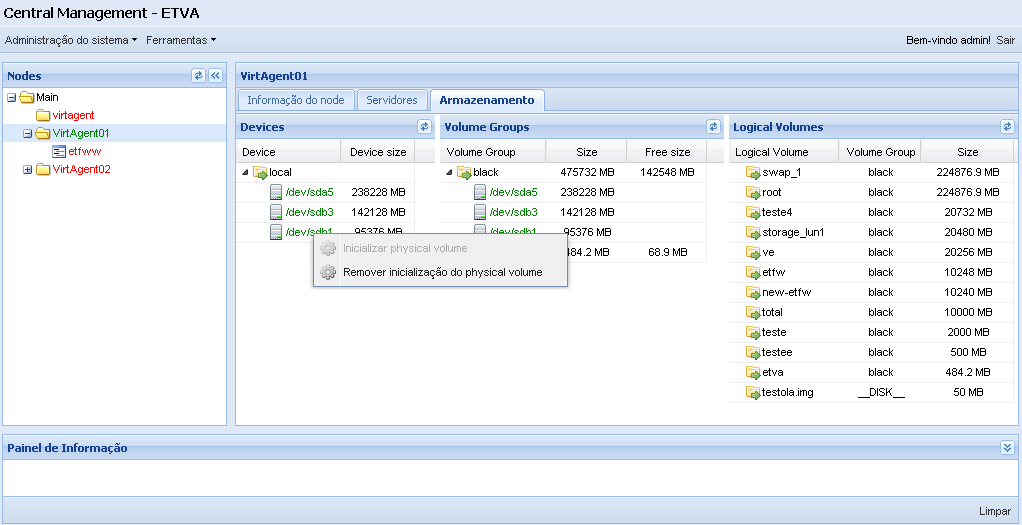
\includegraphics[scale=0.45]{screenshots/node_storage_device_ctx.png}
        \caption{Sub-menu de contexto de um physical volume}
        \label{fig:storage_device_ctx}
        \end{center}
\end{figure}


Para inicializar um \emph{physical volume} acede-se ao sub-menu de contexto do \emph{device} pretendido e seleccionar \emph{Inicializar physical volume}. Para remover um \emph{physical volume} a operação é análoga, bastando seleccionar a opção \emph{Remover inicialização do physical volume} no sub-menu de contexto do \emph{physical volume}.

\begin{quote}
	{\large \bf Nota} \\*[-.8pc]
	\underline{\hspace{6in}} \\
	Só é permitido remover um \emph{physical volume} se este não pertencer a nenhum \emph{volume group}.
\end{quote}

% ADMINISTRAÇÃO VOLUME GROUPS

\subsubsection{Administração de Volume Groups}
Na administração de \emph{volumes groups} é permitido:
\begin{itemize}
	\item Criar um \emph{volume group}
	\item Extender um \emph{volume group}
	\item Reduzir um \emph{volume group}
	\item Remover um \emph{volume group}
\end{itemize}

\begin{figure}[H]
        \begin{center}
        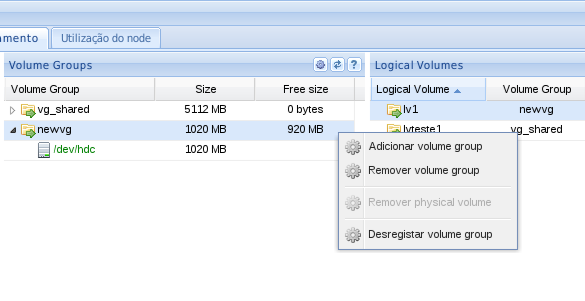
\includegraphics[scale=0.45]{screenshots/node_storage_vg_ctx.png}
        \caption{Sub-menu de contexto de um volume group}
        \label{fig:storage_vg_ctx}
        \end{center}
\end{figure}

Para criar um \emph{volume group} acede-se ao sub-menu de contexto sobre um qualquer \emph{volume group} e seleccionar \emph{Adicionar volume group}.
Na janela de criação deverá ser introduzido o nome pretendido e seleccionar um ou mais \emph{physical voumes} disponíveis.

Um \emph{physical volume} está disponível quando não está alocado a nenhum \emph{volume group} e encontra-se inicializado.

\begin{figure}[H]
        \begin{center}
        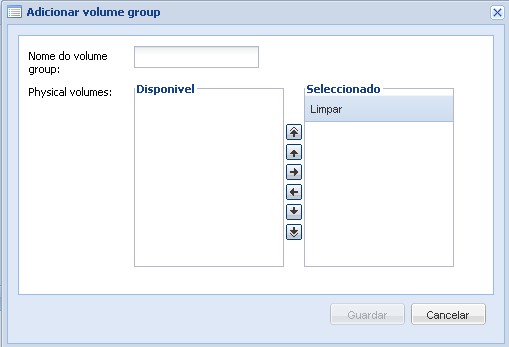
\includegraphics[scale=0.5]{screenshots/storage_vg_create.png}
        \caption{Janela de criação de um volume group}
        \label{fig:storage_vg_create}
        \end{center}
\end{figure}

Para extender um \emph{volume group} recorre-se ao \emph{drag-n-drop}, ou seja, arrasta-se o \emph{physical volume}, que se pretende adicionar, para cima do \emph{volume group} pretendido.

Na remoção/redução de um \emph{volume group} seleccciona-se o \emph{volume group}/\emph{physical volume} a remover e escolhe-se a opção correspondente do sub-menu de contexto.
\begin{quote}
	{\large \bf Nota} \\*[-.8pc]
	\underline{\hspace{6in}} \\
	Só é permitido remover um \emph{volume group} se não houver nenhum \emph{logical volume} associado ao \emph{volume group}.
\end{quote}
 
\begin{figure}[H]
        \begin{center}
        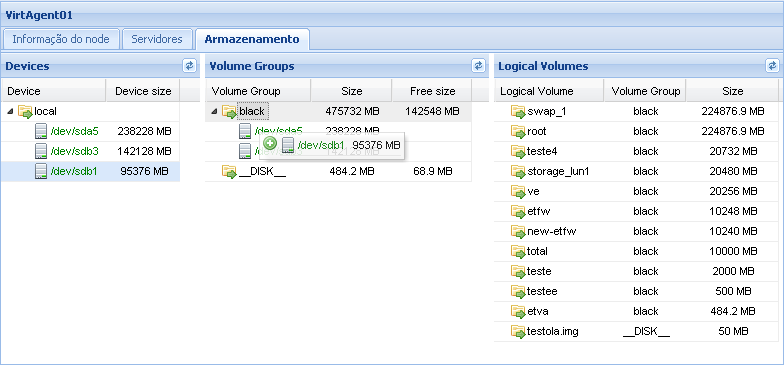
\includegraphics[scale=0.45]{screenshots/storage_vg_extend.png}
        \caption{Extensão de um volume group}
        \label{fig:storage_vg_extend}
        \end{center}
\end{figure}

Na figura \ref{fig:storage_vg_extend} extende-se o \emph{volume group} {\bf black} com o \emph{physival volume} {\bf sdb1}.

% ADMINISTRAÇÃO LOGICAL VOLUMES

\subsubsection{Administração de Logical Volumes}

As operações disponíveis sobre os \emph{logical volumes} são as seguintes:
\begin{itemize}
	\item Criar um \emph{logical volume}
	\item Redimensionar um \emph{logical volume}
	\item Remover um \emph{logical volume}
\end{itemize}

\begin{figure}[H]
        \begin{center}
        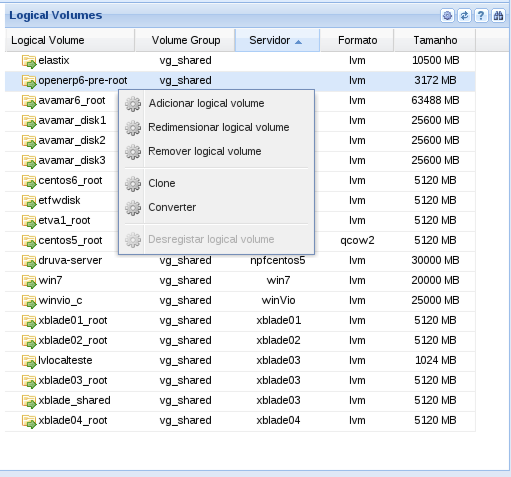
\includegraphics[scale=0.45]{screenshots/node_storage_lv_ctx.png}
        \caption{Sub-menu de contexto de um logical volume}
        \label{fig:storage_lv_ctx}
        \end{center}
\end{figure}

Para criar um \emph{logical volume} acede-se ao sub-menu de contexto sobre um qualquer \emph{logical volume} e selecciona-se \emph{Adicionar logical volume}.
Na janela de criação deverá ser introduzido o nome pretendido, o \emph{volume group} a partir do qual se criará e o tamanho que não deverá exceder o tamanho disponível no \emph{volume group}.

\begin{figure}[H]
        \begin{center}
        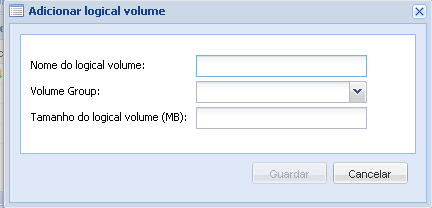
\includegraphics[scale=0.5]{screenshots/storage_lv_create.png}
        \caption{Janela de criação de um logical volume}
        \label{fig:storage_lv_create}
        \end{center}
\end{figure}

No redimensionamento selecciona-se o \emph{logical volume} que se pretende redimensionar e acede-se ao sub-menu de contexto. Aí existe a opção \emph{Redimensionar logical volume} que permite aumentar/reduzir o tamanho do \emph{logical volume}.


\begin{quote}
	{\large \bf Nota} \\*[-.8pc]
	\underline{\hspace{6in}} \\
	Ao reduzir o tamanho do \emph{logical volume} poderá tornar os dados existentes inutilizados. É da responsabilidade do utilizador verificar se é comportável/seguro o redimensionamento do \emph{logical volume} sem afectar os dados nele contidos.
\end{quote}


\begin{figure}[H]
        \begin{center}
        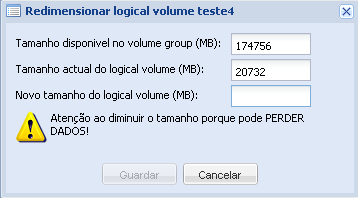
\includegraphics[scale=0.5]{screenshots/storage_lv_resize.png}
        \caption{Redimensionamento de um logical volume}
        \label{fig:storage_lv_resize}
        \end{center}
\end{figure}

Na remoção de um \emph{logical volume}, no sub-menu de contexto existe a opção \emph{Remover logical volume}. O \emph{logical volume} só será removido se não tiver associado a nenhuma máquina virtual. Para verificar se está em uso passa-se o rato por cima do \emph{logical volume} e observar a informação contida no \emph{tooltip} que aparece.

\pagebreak

\section{Máquina virtual}
\label{sec:server}

No painel \emph{Nodes} é possível seleccionar a máquina virtual sobre o qual pretendemos efectuar operações como:

\begin{itemize}
        \item Gestão da máquina virtual
        \item Visualizar estatísticas        
        \item Gestão dos serviços do \emph{Management Agent}
\end{itemize}

\subsection{Informação do servidor}
Em \emph{Informação do servidor} podemos ver o estado da máquina virtual e, entre outras informações, o estado do \emph{Management Agent}.
Para além de visualizar informação, este painel permite efectuar as seguintes operações:
\begin{itemize}
	\item Adicionar máquina virtual (ver secção \ref{sec:add_server})
    \item Editar máquina virtual (ver secção \ref{sec:edit_server})
	\item Remover máquina virtual (ver secção \ref{sec:remove_server})
	\item Abrir máquina virtual numa consola VNC (ver secção \ref{sec:open_vnc})
	\item Iniciar/parar máquina virtual (ver secção \ref{sec:start_server})
    \item Migrar máquina virtual (ver secção \ref{sec:migrate_server})
\end{itemize}

\begin{figure}[H]
	\begin{center}
	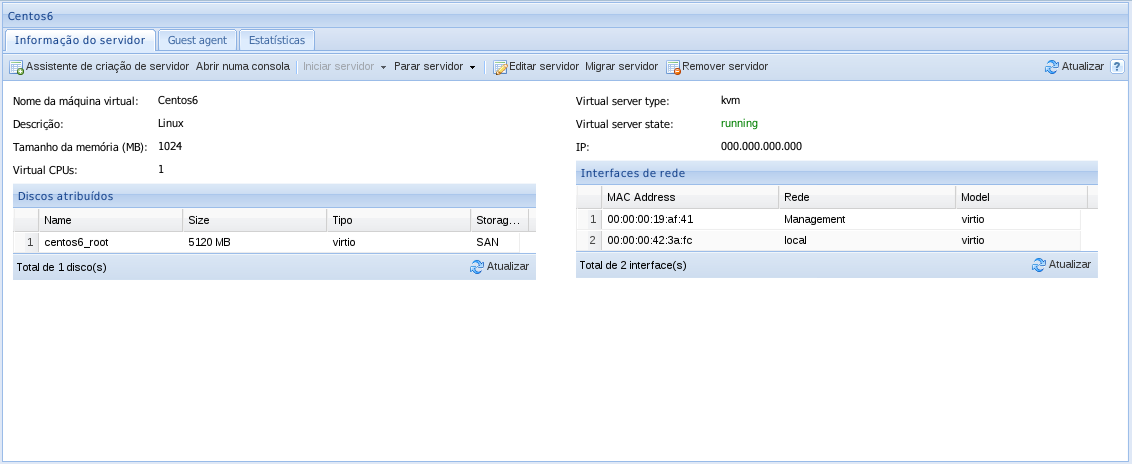
\includegraphics[scale=0.45]{screenshots/server_info.png}
	\caption{Informação da máquina virtual \emph{etfww}}
	\label{fig:server_info}
	\end{center}
\end{figure}

\subsection{Estatísticas}
Em \emph{Estatísticas} é possível visualizar gráficamente informação de:
\begin{itemize}
	\item Cpu Usage
	\item Networks
	\item Memory Usage
	\item Disk
	\item Node Load
\end{itemize}


\begin{figure}[H]
	\begin{center}
	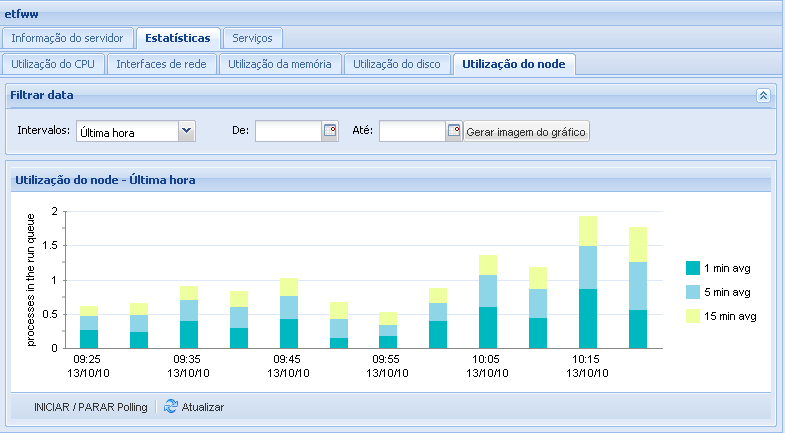
\includegraphics[scale=0.45]{screenshots/server_stats_nodeLoad.png}
	\caption{Estatísticas de uma máquina virtual}
	\label{fig:server_stats_nodeLoad}
	\end{center}
\end{figure}

Em cada um destes paineis é possível visualizar os dados pelos intervalos pré-definidos:
\begin{itemize}
	\item Última hora
	\item Últimas 2 horas
	\item Últimas 24 horas
	\item Última semana
\end{itemize}

Na figura \ref{fig:server_stats_nodeLoad}, visualiza-se a informação de carga do node a que pertence o servidor \emph{etfww} para o intervalo - \emph{Última hora}.

Para visualizar outros intervalos de tempo usa-se \emph{Gerar imagem do gráfico}. A imagem gerada é conforme a figura \ref{fig:server_stats_nodeLoadRange}.
\begin{figure}[H]
	\begin{center}
	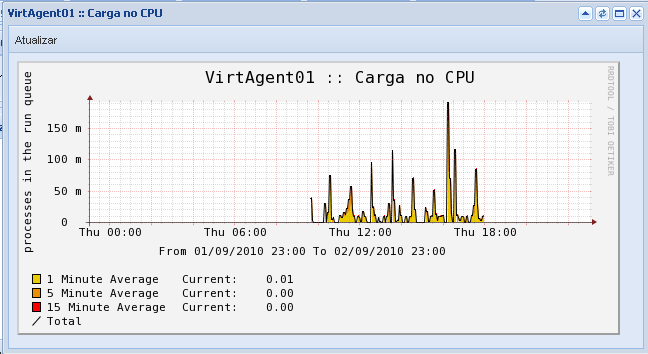
\includegraphics[scale=0.5]{screenshots/server_stats_nodeLoadRange.png}
	\caption{Estatísticas de \emph{Utilização do node} - Carga no CPU}
	\label{fig:server_stats_nodeLoadRange}
	\end{center}
\end{figure}

\subsection{Serviços}
Em \emph{Serviços}, e caso esteja configurado um MA (\emph{Management Agent}) no servidor, é disponibilizada a respectiva configuração dos serviços controlados por esse MA.

\section{Ferramentas}

No menu \emph{Ferramentas} é possível aceder às seguintes ferramentas:
\begin{itemize}
\item Importar OVF
\item Exportar OVF
\item Gestor de ISOs
\item Monitorização do agente dos nodes
\item Registo de eventos do sistema
\end{itemize}

\subsection{Importar OVF}
Esta ferramenta permite importar máquinas virtuais no formato OVF (\emph{Open Virtualization Format}).

\begin{figure}[H]
	\begin{center}
	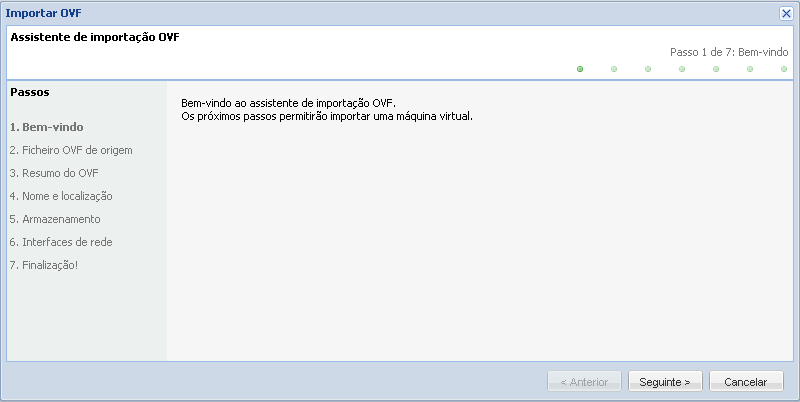
\includegraphics[scale=0.5]{screenshots/ovf_import.png}
	\caption{Assistente de importação OVF - Bem-vindo}
	\label{fig:ovf_import_wiz}
	\end{center}
\end{figure}

O assistente de importação OVF é constituido pelas seguintes etapas:

\begin{description}
	\item[Ficheiro OVF de origem:] Nesta etapa define-se o URL do ficheiro OVF a importar (ver figura \ref{fig:ovf_import_file}).
		
        \begin{quote}
            {\large \bf Nota} \\*[-.8pc]
            \underline{\hspace{6in}} \\
            O CM tem que ter acesso via HTTP ao URL especificado.
        \end{quote}

        \begin{figure}[H]
            \begin{center}
            \includegraphics[scale=0.5]{screenshots/ovf_import_file.png}
            \caption{Assistente de importação OVF - Ficheiro OVF de origem}
            \label{fig:ovf_import_file}
            \end{center}
        \end{figure}

	\item[Resumo do OVF:] Detalhes do ficheiro OVF. Disponibiliza informação acerca do produto, versão, tamanho total dos ficheiros referenciados pelo OVF, se disponível.
		\begin{figure}[H]
            \begin{center}
            \includegraphics[scale=0.5]{screenshots/ovf_import_resume.png}
            \caption{Assistente de importação OVF - Resumo do OVF}
            \label{fig:ovf_import_resume}
            \end{center}
        \end{figure}

    \item[Contrato de licença:] Se especificado no ficheiro OVF, esta etapa surgirá com o EULA. Caso contrário, esta etapa será omitida.
		\begin{figure}[H]
            \begin{center}
            \includegraphics[scale=0.5]{screenshots/ovf_import_eula.png}
            \caption{Assistente de importação OVF - Contrato de licença}
            \label{fig:ovf_import_eula}
            \end{center}
        \end{figure}

    \item[Nome e localização:] Nesta etapa define-se o nome da máquina virtual, o node de destino e o tipo de sistema operativo. As opções do sistema operativo variam consoante a especificação do node:
		\begin{itemize}
			\item com XEN e suporte a virtualização por hardware:
			\begin{itemize}
				\item Linux PV
				\item Linux HVM
				\item Windows
			\end{itemize}
 			\item com XEN sem suporte de virtualização por hardware:
			\begin{itemize}
				\item Linux PV
			\end{itemize}
 			\item com KVM
			\begin{itemize}
				\item Linux
				\item Windows
			\end{itemize}
		\end{itemize}

        \begin{figure}[H]
            \begin{center}
            \includegraphics[scale=0.5]{screenshots/ovf_import_name.png}
            \caption{Assistente de importação OVF - Nome e localização}
            \label{fig:ovf_import_name}
            \end{center}
        \end{figure}

        Antes de prosseguir para a próxima etapa, o assistente verifica se os drivers para os discos e para as interfaces de rede mencionados no OVF são suportados pelo servidor de virtualização escolhido.

        Os drivers dos discos suportados para máquinas XEN com ou sem virtualização por hardware são: ide, xen e scsi. Nas máquinas KVM os drivers são: ide, virtio e scsi.

        Os drivers da placa de rede suportados para máquinas em HVM ou KVM são: e1000, rtl8139 e virtio. Numa máquina XEN sem suporte a virtualização nao suporta drivers.

        Caso o servidor de virtualização escolhido não suporte os drivers mencionados no OVF a importação não poderá ser efectuada.


    \item[Armazenamento:] Nesta etapa é efectuado o mapeamento dos discos no node. É possível especificar o nome a dar ao \emph{logical volume} bem como definir o \emph{volume group}.
        É necessário que todo os discos sejam mapeados para prosseguir para a próxima etapa.
		\begin{figure}[H]
            \begin{center}
            \includegraphics[scale=0.5]{screenshots/ovf_import_storage.png}
            \caption{Assistente de importação OVF - Armazenamento}
            \label{fig:ovf_import_storage}
            \end{center}
        \end{figure}    

    \item[Interfaces de rede:] Nesta etapa é efectuado o mapeamento das interfaces de rede. É possível especificar novas interfaces de rede.
        É necessário que todas as interfaces de rede sejam mapeadas para prosseguir para a próxima etapa.
		\begin{figure}[H]
            \begin{center}
            \includegraphics[scale=0.5]{screenshots/ovf_import_networks.png}
            \caption{Assistente de importação OVF - Interfaces de rede}
            \label{fig:ovf_import_networks}
            \end{center}
        \end{figure}

    \item[Finalização!] Etapa final do assistente. Após confirmação da importação da máquina virtual, os dados recolhidos nas etapas anteriores são processados e enviados ao servidor de virtualização. Posteriormente no painel \emph{Servidores} poderá ser iniciada a máquina através da opção \emph{Iniciar servidor}.
		\begin{figure}[H]
			\begin{center}
			\includegraphics[scale=0.5]{screenshots/ovf_import_finish.png}
            \caption{Assistente de importação OVF - Finalização!}
			\label{fig:ovf_import_finish}
			\end{center}
		\end{figure}

\end{description}

\subsection{Exportar OVF}
Esta ferramenta permite exportar máquinas virtuais no formato OVF (\emph{Open Virtualization Format}).
O ficheiro gerado vem no formato OVA (\emph{Open Virtualization Archive}).

\begin{quote}
	{\large \bf Nota} \\*[-.8pc]
	\underline{\hspace{6in}} \\
	A máquina virtual a exportar necessita estar parada para se efectuar a exportação.
\end{quote}

\begin{figure}[H]
	\begin{center}
	\includegraphics[scale=0.5]{screenshots/ovf_export.png}
	\caption{Janela de exportação OVF}
	\label{fig:ovf_export}
	\end{center}
\end{figure}


\subsection{Gestor de ISOs}
Esta ferramenta permite fazer a gestão das imagens que estão disponíveis para uso nas máquinas virtuais.
Os ficheiros existentes servirão posteriormente para serem montadas no \emph{CD-ROM} das máquinas virtuais.

\begin{figure}[H]
	\begin{center}
	\includegraphics[scale=0.5]{screenshots/iso_manager.png}
	\caption{Painel de gestão das ISOs}
	\label{fig:iso_manager}
	\end{center}
\end{figure}

As operações permitidas são:
\begin{itemize}
\item Upload de múltiplos ficheiros
\item Download de ficheiros
\item Renomear ficheiros
\item Apagar ficheiros
\end{itemize}


\begin{quote}
	{\large \bf Nota} \\*[-.8pc]
	\underline{\hspace{6in}} \\
	As alterações efectuadas às imagens existentes, que estejam definidas no arranque por CD-ROM de uma qualquer máquina virtual,
     não se irão reflectir automáticamente. Cabe ao utilizador verificar se a imagem montada no CD-ROM continua válida.
\end{quote}

\subsection{Monitorização do agente dos nodes}
Esta ferramenta serve para verificar em tempo real a comunicação dos vários nodes com o CM. A verificação é feita periódicamente.
Para parar a verificação fecha-se o pop-up que surge aquando da activação da ferramenta.

\subsection{Registo de eventos do sistema}

Em \emph{Registo de eventos do sistema} é possível visualizar as interações efectuadas entre o utilizador, nodes, servidores e o CM.

\begin{figure}[H]
	\begin{center}
	\includegraphics[scale=0.5]{screenshots/events_log.png}
	\caption{Janela do registo de eventos do sistema}
	\label{fig:events_log}
	\end{center}
\end{figure}

As mensagens do registo de eventos podem ser filtradas por três tipos de mensagem:
\begin{itemize}
    \item {\bf Debug} - Apresenta todas as mensagens. Agrega os níveis \emph{Info} e \emph{Error}
    \item {\bf Info} - Mensagens com informação dos eventos que foram bem sucedidos
    \item {\bf Error} - Mensagens com informação dos eventos que não foram bem sucedidos
\end{itemize}

\section{Administração do sistema}
\label{sec:first_time_wizard}
No menu \emph{Administração do sistema} é possível efectuar:
\begin{itemize}
\item Assistente de configuração inicial
\item Alterar preferências
\item Administração de utilizadores e permissões
\end{itemize}

\subsection{Assistente de configuração inicial}
O assistente de configuração inicial reúne o conjunto de operações a efectuar no primeiro acesso ao CM. Permite efectuar uma primeira configuração rápida do sistema.

O assistente de configuração, conforme a figura \ref{fig:first_time_wizard}, consiste nos seguintes passos:
\begin{itemize}
	\item Alteração da password inicial
	\item Geração da MAC pool
	\item Configuração da Rede
\end{itemize}

\begin{figure}[H]
        \begin{center}
        \includegraphics[scale=0.7]{screenshots/first_time_wizard.png}
        \caption{Assistente de configuração inicial (\emph{ETVA Enterprise})}
        \label{fig:first_time_wizard}
        \end{center}
\end{figure}

\begin{quote}
	{\large \bf Nota} \\*[-.8pc]
	\underline{\hspace{6in}} \\
	Caso se trate de um \emph{ETVA Standard} a configuração das redes é omitida.
\end{quote}

\subsection{Alterar preferências}
Acedendo a \emph{Preferências} é possível definir alguns parâmetros globais ao sistema.
No painel \emph{Geral} é permitido especificar o \emph{keymap} usado por omissão no acesso por VNC às máquinas virtuais, bem como definir a duração dos registos de eventos do sistema.

\begin{figure}[H]
        \begin{center}
        \includegraphics[scale=0.5]{screenshots/preferences_general.png}
        \caption{Janela de preferências do sistema - Painel Geral}
        \label{fig:preferences_general}
        \end{center}
\end{figure}

No painel \emph{Conectividade} é permitido alterar o IP do CM e da rede LAN caso se trate de um \emph{ETVA Enterprise}. No modelo \emph{ETVA Enterprise} permite apenas configurar o IP do CM.

\begin{figure}[H]
        \begin{center}
        \includegraphics[scale=0.5]{screenshots/preferences_conn.png}
        \caption{Janela de preferências do sistema - Painel Conectividade}
        \label{fig:preferences_conn}
        \end{center}
\end{figure}

\subsection{Admininstração de utilizadores e permissões}
Na Administração de utilizadores e permissões é possivel fazer a gestão de contas de utilizadores, permissões e grupos.

\begin{figure}[H]
        \begin{center}
        \includegraphics[scale=0.4]{screenshots/user_admin.png}
        \caption{Janela de administração de utilizadores e permissões}
        \label{fig:user_admin}
        \end{center}
\end{figure}

O CM actualmente não suporta diferentes tipos de credenciais\footnote{As credenciais serão implementadas numa futura versão} apesar de ser possível criar vários grupos de utilizadores e permissões.
Todos os utilizadores podem efectuar a gestão de utilizadores e permissões.

\begin{quote}
	{\large \bf Nota} \\*[-.8pc]
	\underline{\hspace{6in}} \\    
	Em \emph{Gestão de Grupos} não é possível remover o grupo com ID 1 dado ser o grupo por omissão do sistema.
\end{quote}

\pagebreak
\chapter{\textsf{ETVA Management Agents}}

Com o ETVA é possível gerir via interface web os serviços de algumas soluções Eurotux nomeadamente:
\begin{itemize}
	\item ETFW - Solução de Firewall
	\item ETMS - Solução de Mail Server
	\item ETVOIP - Solução de VOIP
\end{itemize}
    
    
A gestão dos serviços é possível através da instalação e configuração de agentes de gestão (\emph{Management Agents}) nas máquinas virtuais onde correm as respectivas soluções.

%\section{ETFW}
\section{ETFW}
In a virtual machine with the image of \textit{ETFW} you can configure the service via Central Management, on tab \textit{ETFW}.

In the main panel you can access the \textit{Network setup wizard} or access the \textit{Webmin} interface to make changes in any configuration.

The site also has the \textit{Save configuration} option that makes the changes effective. Without this option, any changes made lost after \textit{reboot}.

\begin{figure}[H]
    \begin{center}
    \includegraphics[scale=0.38]{screenshots/etfw/etfwmain.png}
    \caption{Main panel}
    \label{fig:etfwmain}
    \end{center}
\end{figure}

\subsection{Network setup Wizard}

To configure the module \textit{ETFW} quickly and efficiently it's provided a step by step setup wizard.

\begin{figure}[H]
    \begin{center}
    \includegraphics[scale=0.38]{screenshots/etfw/etfw_wizard_01.png}
    \caption{Welcome}
    \label{fig:etfw_wizard_passo1}
    \end{center}
\end{figure}

\begin{figure}[H]
    \begin{center}
    \includegraphics[scale=0.38]{screenshots/etfw/etfw_wizard_02.png}
    \caption{Topology setup}
    \label{fig:etfw_wizard_passo2}
    \end{center}
\end{figure}

\begin{figure}[H]
    \begin{center}
    \includegraphics[scale=0.38]{screenshots/etfw/etfw_wizard_03.png}
    \caption{Configuring the WAN interface}
    \label{fig:etfw_wizard_passo3}
    \end{center}
\end{figure}

\begin{figure}[H]
    \begin{center}
    \includegraphics[scale=0.38]{screenshots/etfw/etfw_wizard_04.png}
    \caption{Configuring the LAN interface}
    \label{fig:etfw_wizard_passo4}
    \end{center}
\end{figure}

\begin{figure}[H]
    \begin{center}
    \includegraphics[scale=0.38]{screenshots/etfw/etfw_wizard_05.png}
    \caption{Configuring of the DHCP service for LAN network}
    \label{fig:etfw_wizard_passo5}
    \end{center}
\end{figure}

\begin{figure}[H]
    \begin{center}
    \includegraphics[scale=0.38]{screenshots/etfw/etfw_wizard_06.png}
    \caption{Configuring SQUID proxy}
    \label{fig:etfw_wizard_passo6}
    \end{center}
\end{figure}

\begin{figure}[H]
    \begin{center}
    \includegraphics[scale=0.38]{screenshots/etfw/etfw_wizard_07.png}
    \caption{Configuring DMZ interface}
    \label{fig:etfw_wizard_passo7}
    \end{center}
\end{figure}

\begin{figure}[H]
    \begin{center}
    \includegraphics[scale=0.38]{screenshots/etfw/etfw_wizard_08.png}
    \caption{Configuring DHCP service for DMZ network}
    \label{fig:etfw_wizard_passo8}
    \end{center}
\end{figure}

\begin{figure}[H]
    \begin{center}
    \includegraphics[scale=0.38]{screenshots/etfw/etfw_wizard_09.png}
    \caption{Completion of the configuration}
    \label{fig:etfw_wizard_passo9}
    \end{center}
\end{figure}

\subsection{Network setup - \textit{Network}}
In addition to the wizard configuration process you can change the network configuration manually.
To do this, go to the \textit{network} tab where we have access to the configuration of network interfaces (\textit{Network interfaces}), routing rules (\textit{Routing and gateways}), address configuration (\textit{Host Addresses}) and client \textit{DNS} (\textit{Hostname and DNS client}).

\subsubsection{Network interfaces}
In \textit{Network interfaces} we can see the network interfaces that are configured and which are going to be active at the machine start.

When selecting an interface we can edit the parameters of the interface, such as the IP address, netmask, broadcast, and aliases in virtual interfaces.
To add a new interface, select the add button and fill in the required fields for the interface configuration.

\begin{figure}[H]
    \begin{center}
    \includegraphics[scale=0.38]{screenshots/etfw/etfw_network_interfaces_01.png}
    \caption{Active interfaces}
    \label{fig:etfw_network_interfaces_01}
    \end{center}
\end{figure}

\begin{figure}[H]
    \begin{center}
    \includegraphics[scale=0.38]{screenshots/etfw/etfw_network_interfaces_02.png}
    \caption{After boot active interfaces}
    \label{fig:etfw_network_interfaces_02}
    \end{center}
\end{figure}

If you wish to define an alias for a network interface, you must select the desired interface, edit and choose \textit{Add virtual} in \textit{Virtual interfaces}. Next, fill out the required parameters and save.

\begin{figure}[H]
    \begin{center}
    \includegraphics[scale=0.38]{screenshots/etfw/etfw_network_interfaces_03.png}
    \caption{Alias interface}
    \label{fig:etfw_network_interfaces_02}
    \end{center}
\end{figure}

\begin{figure}[H]
    \begin{center}
    \includegraphics[scale=0.38]{screenshots/etfw/etfw_network_interfaces_04.png}
    \caption{Alias interface active at boot}
    \label{fig:etfw_network_interfaces_02}
    \end{center}
\end{figure}

\subsubsection{Routing and gateways}
In \textit{Routing and gateways} we can query the active routing rules and remove or add new rules.
We can also define routing rules that are set at startup.

\begin{figure}[H]
    \begin{center}
    \includegraphics[scale=0.38]{screenshots/etfw/etfw_network_routing_01.png}
    \caption{Active forwarding rules}
    \label{fig:etfw_network_routing_01}
    \end{center}
\end{figure}

To create a routing rule, we choose the \textit{add} option and define the parameters of the route:

\begin{itemize}
    \item \textit{Route destination} - Destination of the forwarding route. It can be \textit{default}, destination IP address or network address;
    \item \textit{Netmask for destination} - Netmask for the route of destination;
    \item \textit{Route via} - \textit{Gateway} or network interface of output route.
\end{itemize}

\begin{figure}[H]
    \begin{center}
    \includegraphics[scale=0.38]{screenshots/etfw/etfw_network_routing_02.png}
    \caption{Defined routing rules at startup}
    \label{fig:etfw_network_routing_02}
    \end{center}
\end{figure}

In the routing rules defined at startup we can configure the following rule types:
\begin{itemize}
    \item \textit{Default routes} - to define the default gateway;
    \item \textit{Static routes} - static routes to other networks/machines;
    \item \textit{Local routes} - static routes where IP addresses are defined, netmask and the interface of each route.
\end{itemize}

\subsubsection{Host Addresses}
In \textit{Host Addresses} you can define static names and locals, associated with IP addresses, in order to reduce response time in name resolution.

\begin{figure}[H]
    \begin{center}
    \includegraphics[scale=0.38]{screenshots/etfw/etfw_network_hostaddresses_01.png}
    \caption{Address setup}
    \label{fig:etfw_network_hostaddresses_01}
    \end{center}
\end{figure}

\subsubsection{Hostname and DNS Client}
From this option you can set the name that the machine will have locally and the configuration parameters of the DNS client service (DNS server addresses, order of name resolution on addresses and search domains names).

\begin{figure}[H]
    \begin{center}
    \includegraphics[scale=0.38]{screenshots/etfw/etfw_network_dnsclient_01.png}
    \caption{DNS client}
    \label{fig:etfw_network_dnsclient_01}
    \end{center}
\end{figure}

\subsection{Firewall rules}
By accessing the tab \textit{Firewall} we have the ability to set the rules of Firewall.
This firewall is based on \textit{iptables}, formed by three basic objects:

\begin{itemize}
    \item Rules
    \item Chains
    \item Tables
\end{itemize}

The rules are lower-level objects that perform packet filtering or manipulation.
A rule consists of the following parts:

\begin{itemize}
\item The table were the rule will be added;
\item The chain chain to which the rule will be added;
\item The filtering or manipulation instructions.
\end{itemize}

The rules are organized in chains and act as a checklist of rules ordered.

The chains are organized in tables that group a large number of possible rules to filter and/or manipulate packets.

The operation of the firewall proceeds as follows: if the packet header meet the requirements of the rule, this will follow the destiny imposed by the rule, otherwise it will be evaluated further by the next rule.
%When there are no more rules will be applied the package the default rule or standard set.

\begin{figure}[H]
    \begin{center}
    \includegraphics[scale=0.38]{screenshots/etfw/etfw_firewall_01.png}
    \caption{Firewall: Filter table}
    \label{fig:etfw_firewall_01}
    \end{center}
\end{figure}

By accessing the firewall tab the interface shows three tables: \textit{Packet alteration} - \textit{mangle}, \textit{Network address translation} - \textit{nat} and \textit{Packet filtering} - \textit{filter}.

\subsubsection{Table \textit{Filter} - \textit{Packet Filtering}}
The table \textit{filter} is used to filter packets that pass through the firewall and presents three firewall pre-defined chains:

\begin {itemize}
   \item \textbf{INPUT} - filter packets whose destination is the own firewall;
   \item \textbf{OUTPUT} - filters packets whose origin is firewall;
   \item \textbf{FORWARD} - filter packets that pass through the firewall which are not the source nor the destination of the firewall.
\end {itemize}

\begin{figure}[H]
    \begin{center}
    \includegraphics[scale=0.38]{screenshots/etfw/etfw_firewall_02.png}
    \caption{Creating a rule on table \textit{filter} - Chain and action}
    \label{fig:etfw_firewall_02}
    \end{center}
\end{figure}

When creating a rule in a filter table's chain some parameters are required for action to take:

\begin{itemize}
   \item \textbf{Rule comment} - allows you to write a short comment to identify the rule to be created;
   \item \textbf{Action to take} - action to be taken, who decides what should be done with the package, if it matches the rule. The most important actions are:
       \subitem \textbf{Drop} - removes the packet without doing anything else;
       \subitem \textbf{Accept} - the firewall lets the packet pass through and the data is sent to the recipient;
       \subitem \textbf{Reject} - works the same way as the drop but is sent an \textit {ICMP} error back to the sender of the package;
       \subitem \textbf{Userspace} - if this option is active, a multicast is donne by kernel into a socket where can be a listening process.
\end{itemize}

\begin{figure}[H]
    \begin{center}
    \includegraphics[scale=0.38]{screenshots/etfw/etfw_firewall_03.png}
    \caption{Creating a rule on table \textit{filter} - Condition details}
    \label{fig:etfw_firewall_03}
    \end{center}
\end{figure}

Other options that can be completed in the condition are the following:
\begin{itemize}
    \item \textbf{Source address or network} - Network address that establish the origin of the package. It is usually a combination of IP address with the subnet mask separated by a slash (eg 192.168.1.0/255.255.255.0 or 192.168.1.0/24);
    \item \textbf{Destination address or network} - Network address to which the packet is intended. It has the same combination as before;
    \item \textbf{Incoming interface} - Specifies the input interface of the package;
    \item \textbf{Outgoing interface} - Specifies the output interface of the package;
    \item \textbf{Fragmentation} - Sometimes a packet undergoes fragmentation because of its size, being its part joined together later in the destination. This option sets whether the rule is matched by fragmented packets or not;
    \item \textbf{Network protocol} - Network protocol;
    \item \textbf{Source TCP or UDP port} - Sets the match rule with the incoming port (tcp or udp), and may be defined a range of ports (example: 1000:1050) or a list doors separated by commas;
    \item \textbf{Destination TCP or UDP port} - Sets the output port match and may be offered a range of ports (example: 1000:1050) or a list of ports separated by commas;
    \item \textbf{Source and destination port(s)} - Sets the door match, both incoming and outgoing, may be offered a range of ports or a list of ports separated by commas;
    \item \textbf{ICMP packet type} - ICMP packet type;
    \item \textbf{Ethernet address} - Defines a physical address of a network that will serve to match the rule;
    \item \textbf{Packet flow rate} - Sets the volume of packages that will make the rule match;
    \item \textbf{Packet burst rate} - Sets the threshold at which the packets begin to make match with the rule;
    \item \textbf{Connection states} - Specifies the number of links that make the rule match;
    \item \textbf{Type of service} - Defines the type of service for which we want the rule to do match;
    \item \textbf{Additional parameters} - Specifies additional parameters that will be passed directly to the line of the rule to be applied.
\end{itemize}

\subsubsection{NAT table - Network address translation}
The NAT table is used for network address translation, or translate a package with a particular field of origin or destination.
Only the first packet will be affected by this chain, after which the remaining packages will apply the same actions as the first.
This table presents three pre-defined chains:

\begin{itemize}
    \item \textbf{PREROUTING} - applies the changes to the packages when the target needs to be changed;
    \item \textbf{POSTROUTING} - applies the changes to the packages when the source needs to be changed;
    \item \textbf{OUTPUT} - applies the changes to packets originated by the firewall.
\end{itemize}

The current targets in this table are:

\begin{itemize}
    \item \textbf{DNAT} - used in cases where you have a public IP address in the firewall and if you want to redirect the access to another host (a DMZ for example), thus allowing forward traffic.
    \item \textbf{SNAT} - used when you want to change the origin of package, usually to hide the addresses of local network or \textit{DMZ}.
    \item \textbf{MASQUERADE} - used the same way that the SNAT and for the same reason, but the outgoing IP address is not specified, by using the source address of the interface package. This rule is used primarily for dynamic IP addresses, because if the link goes down, the source address that was being used is discarded yielding place to a new source address of the interface when the connection is restored.
\end{itemize}

\begin{figure}[H]
    \begin{center}
    \includegraphics[scale=0.38]{screenshots/etfw/etfw_firewall_04.png}
    \caption{Creating a rule on NAT table}
    \label{fig:etfw_firewall_03}
    \end{center}
\end{figure}

The options used in the NAT table are identical to the Filter table. The differences are listed bellow:

\begin{itemize}
    \item \textbf{Action to take} - action to be taken, has the same functionality described in the Filter table, but has two different options:
        \subitem \textbf{Masquerade} - Rewrites the outgoing IP address, when it comes to dynamic IP addresses;
        \subitem \textbf{Source NAT} / \textbf{Destination NAT} - Depending on the chain (PREROUTING, POSTROUTING or OUTPUT), available options may vary. They will be \textit{Source NAT} and \textit{estination NAT}, respectively. Also, they will re-write the IP's input and output respectively.
\end{itemize}

\subsubsection{Mangle table - Packet alteration}

This table is not addressed in this version of the manual.

\subsection{DHCP Server}
In this tab we can configure the DHCP server, including IP range to allocate the hosts, router address, DNS server address, view active leases, and to start/stop the server.

\begin{figure}[H]
    \begin{center}
    \includegraphics[scale=0.38]{screenshots/etfw/etfw_dhcp_wizard_01.png}
    \caption{IP range setup}
    \label{fig:etfw_dhcp_wizard_01}
    \end{center}
\end{figure}

From the DHCP Wizard we can, in a first stage, set the IP ranges allocated to hosts.

\begin{figure}[H]
    \begin{center}
    \includegraphics[scale=0.38]{screenshots/etfw/etfw_dhcp_subnets_01.png}
    \caption{Subnets setup}
    \label{fig:etfw_dhcp_subnets_01}
    \end{center}
\end{figure}

\begin{figure}[H]
    \begin{center}
    \includegraphics[scale=0.38]{screenshots/etfw/etfw_dhcp_subnets_02.png}
    \caption{Subnet edit}
    \label{fig:etfw_dhcp_subnets_02}
    \end{center}
\end{figure}

Later, you can edit the subnets and set the appropriate parameters to our setting for the network address, netmask, address range, among others.

\begin{figure}[H]
    \begin{center}
    \includegraphics[scale=0.38]{screenshots/etfw/etfw_dhcp_interfaces_01.png}
    \caption{Choose an interface}
    \label{fig:etfw_dhcp_interfaces_01}
    \end{center}
\end{figure}

To configure the server properly you must set the interface on which service will operate.
Go to \textit{Edit Network Interface} and choose the desired network interface.

\begin{figure}[H]
    \begin{center}
    \includegraphics[scale=0.38]{screenshots/etfw/etfw_dhcp_texteditor_01.png}
    \caption{Configuration file edition}
    \label{fig:etfw_dhcp_texteditor_01}
    \end{center}
\end{figure}

Additionally, you can always view and edit the configuration file directly and put the desired options.

\begin{figure}[H]
    \begin{center}
    \includegraphics[scale=0.38]{screenshots/etfw/etfw_dhcp_leases_01.png}
    \caption{List of active leases}
    \label{fig:etfw_dhcp_leases_01}
    \end{center}
\end{figure}

In any time you can find a list of assigned IPs by selecting the option \textit{List active leases}. This option is also available for each subnet.

\subsection{SQUID server}

In the \textit{SQUID Server} tab you can configure the SQUID Proxy service.

\begin{figure}[H]
    \begin{center}
    \includegraphics[scale=0.38]{screenshots/etfw/etfw_squid_wizard_01.png}
    \caption{SQUID server setup}
    \label{fig:etfw_squid_wizard_01}
    \end{center}
\end{figure}

The proxy service forward requests to the Internet and keeps a content's cache in a way to speed up the display when they are requested again.

In the \textit{SQUID Wizard} we can configure the proxy service easily. It has three pre-defined configuration options:

\begin{itemize}
    \item \textit{Transparent Proxy} - Transparent Proxy;
    \item \textit{Proxy with AD} - Proxy with authentication in Active Directory;
    \item \textit{Proxy with LDAP} - Proxy with LDAP authentication.
\end{itemize}

In the first case, the transparent proxy, allows you to have a cache system cache completely invisible to the customers. This system does not support authentication.

In the other two cases, the proxy makes use of authentication systems, such as Active Directory or LDAP.

Additionally, you can customize the service in accordance with the needs, in particular define: Ports and Networking, Access Control, Authentication Programs, among other types of cache.

\subsubsection{Ports and Networking}

In \textit{Ports and Networking} you can define the port (SSL or not), and IP address or hostname of the proxy service that will fill orders, in addition to other possible configurations, including:

\begin{figure}[H]
    \begin{center}
    \includegraphics[scale=0.38]{screenshots/etfw/etfw_squid_portsnetworking_01.png}
    \caption{Port and network configuration}
    \label{fig:etfw_squid_portsnetworking_01}
    \end{center}
\end{figure}

Request port \textit{ICP};
Validation name addresses of URLs;
Specification group \textit{multicast};
Output address of TCP traffic;
Output address UDP traffic;


\begin{itemize}
    \item \textit{ICP port} - ICP request port;
    \item \textit{Validate hostnames in URLs?} - Validation of urls' address;
    \item \textit{Multicast groups} - Multicast groups;
    \item \textit{Outgoing TCP address} - Output address for TCP traffic;
    \item \textit{Outgoing UDP address} - Output address for UDP traffic;
    \item \textit{Incoming UDP address} - Input address for UDP traffic;
    \item \textit{TCP receive buffer} - Buffer \textit{TCP};
\end{itemize}

\subsubsection{Access Control}

The access control policies are based on a combination of \textit{ACL}(\textit{Access Control Lists}).

\begin{figure}[H]
    \begin{center}
    \includegraphics[scale=0.38]{screenshots/etfw/etfw_squid_accesscontrol_01.png}
    \caption{Setup of access control policies}
    \label{fig:etfw_squid_accesscontrol_01}
    \end{center}
\end{figure}

In the configuration of access control policies we can define filtering models that can be used later in the sections of restrictions of access (\textit{Proxy Restrictions}, \textit{ICP Restrictions}, \textit{Proxy Reply Restrictions}) .

\begin{figure}[H]
    \begin{center}
    \includegraphics[scale=0.38]{screenshots/etfw/etfw_squid_accesscontrol_02.png}
    \caption{Creating a new ACL}
    \label{fig:etfw_squid_accesscontrol_02}
    \end{center}
\end{figure}

To create a new ACL, we select the type and fill with the desired parameters.

\begin{figure}[H]
    \begin{center}
    \includegraphics[scale=0.38]{screenshots/etfw/etfw_squid_accesscontrol_03.png}
    \caption{Creating a new external acl}
    \label{fig:etfw_squid_accesscontrol_03}
    \end{center}
\end{figure}

It is also possible to define external ACLs that allow to expand the functionalities of the proxy, using for this purpose external programs that manage the access.
These ACLs allow, for example, the authentication in a server such as a Active Directory or a LDAP, or even the verification of source addresses in a SQL database.

The creation of an external \textit{ACL} external requires the creation of an internal ACL with reference to the first one.

\begin{figure}[H]
    \begin{center}
    \includegraphics[scale=0.38]{screenshots/etfw/etfw_squid_accesscontrol_04.png}
    \caption{Restriction definition - \textit{Proxy restrictions}}
    \label{fig:etfw_squid_accesscontrol_04}
    \end{center}
\end{figure}

After the ACL definition, you must associate the restrictions with the ACLs to be applied in every situation, or what action to do: accept or deny.
The rules are applied in top-bottom order, and when a match is found the action takes place.
Importantly, if there is a deny all rule, all requests that pass the rules are accepted.

\subsubsection{Authentication Programs}

In \textit{Authentication Programs} are defined programs that ask the browser/user what's his authentication credentials.

\begin{figure}[H]
    \begin{center}
    \includegraphics[scale=0.38]{screenshots/etfw/etfw_squid_authenticationprograms_01.png}
    \caption{Authentication Programs}
    \label{fig:etfw_squid_authenticationprograms_01}
    \end{center}
\end{figure}

There are two types of authentication:

\begin{itemize}
    \item \textit{Basic} - when the browser does not support transparent authentication, it will show a popup asking the user credentials
    \item \textit{NTLMSSP} - transparent authentication for the user
\end{itemize}

We can even set the following parameters:

\begin{itemize}
    \item \textit{authentication program} - Specifies the user program for authentication. The program reads a line containing user and the password separated by space, and responds \textit{OK} on success or \textit{ERR} on failure;
    \item \textit{Number of authentication programs} - Maximum number of process that the authentication could have;
    \item \textit{Authentication realm} - Text that will appear in the dialog box in case of basic authentication;
    \item \textit{Authentication cache time} - Specifies how long a valid authentication is maintained avoiding requests;
    \item \textit{Number of times an NTLM challenge can be re-used} - A maximum number of times that can be used in NTLMSSP authentication type;
    \item \textit{Lifetime of NTLM challenges} - Lifetime of the \textit{NTLMSSP} authentication type;
    \item \textit{Authenticate IP cache time} - Specifies for how long the cache is kept about the user-IP association. 
\end{itemize}

\subsubsection{Other Caches}

In \textit{Other caches} we can specify other proxies to be used in a chain the get information.

\begin{figure}[H]
    \begin{center}
    \includegraphics[scale=0.38]{screenshots/etfw/etfw_squid_othercaches_01.png}
    \caption{Proxies - Other Caches}
    \label{fig:etfw_squid_othercaches_01}
    \end{center}
\end{figure}

\begin{figure}[H]
    \begin{center}
    \includegraphics[scale=0.38]{screenshots/etfw/etfw_squid_othercaches_02.png}
    \caption{Edit host cache}
    \label{fig:etfw_squid_othercaches_01}
    \end{center}
\end{figure}

To specify a different proxy it's necessary to specify the following fields:

\begin{itemize}
    \item \textit{Hostname} - IP address or hostname (\textit{FQDN}) of the cache to being used;
    \item \textit{Type} - Type hierarchy to be used between the proxies:
        \subitem \textit{parent};
        \subitem \textit{sibling};
        \subitem \textit{multicast};
    \item \textit{Proxy port} - The port that proxy uses for listening requests;
    \item \textit{ICP port} - Used port to ask neighbors about the cache objects that they have;
    \item \textit{Proxy only?} - Indicates that the requested content to this proxy is not to save locally; 
    \item \textit{Send ICP queries} - Used for proxies that does not have ICP, i.e., that indicates if they have a object or not;
    \item \textit{Default cache} - It is used when the proxy is the last in the hierarchy line;
    \item \textit{Round-robin cache} - To use the round-robin algorithm of search for proxies;
    \item \textit{ICP time-to-live} - Specifies the Time-To-Live(ttl) used in multicast protocol;
    \item \textit{Cache weighting} - Specifies the importance of the cache on the process o choosing proxy (1 for lower priority).
\end{itemize}

\subsubsection{Usage exemples}

\begin{figure}[H]
    \begin{center}
    \includegraphics[scale=0.38]{screenshots/etfw/etfw_squid_example_time_01_01.png}
    \caption{Restrict internal network access only during work hours - Creating ACLs.}
    \label{fig:etfw_squid_example_time_01_01}
    \end{center}
\end{figure}

\begin{figure}[H]
    \begin{center}
    \includegraphics[scale=0.38]{screenshots/etfw/etfw_squid_example_time_01_02.png}
    \caption{Restrict internal network access only during work hours - Creating restriction using previously defined ACLs}
    \label{fig:etfw_squid_example_time_01_02}
    \end{center}
\end{figure}

\begin{figure}[H]
    \begin{center}
    \includegraphics[scale=0.38]{screenshots/etfw/etfw_squid_example_time_02_01.png}
    \caption{Restrict access only in the morning - Creating ACLs}
    \label{fig:etfw_squid_example_time_02_01}
    \end{center}
\end{figure}

\begin{figure}[H]
    \begin{center}
    \includegraphics[scale=0.38]{screenshots/etfw/etfw_squid_example_time_02_02.png}
    \caption{Restrict access only in the morning - Creating restriction using previously defined ACLs}
    \label{fig:etfw_squid_example_time_02_02}
    \end{center}
\end{figure}

\begin{figure}[H]
    \begin{center}
    \includegraphics[scale=0.38]{screenshots/etfw/etfw_squid_example_acessoip_01.png}
    \caption{Restrict access by IP address - Creating ACLs}
    \label{fig:etfw_squid_example_acessoip_01}
    \end{center}
\end{figure}

\begin{figure}[H]
    \begin{center}
    \includegraphics[scale=0.38]{screenshots/etfw/etfw_squid_example_acessoip_02.png}
    \caption{Restrict access by IP address - Creating restriction using previously defined ACLs}
    \label{fig:etfw_squid_example_acessoip_02}
    \end{center}
\end{figure}

\begin{figure}[H]
    \begin{center}
    \includegraphics[scale=0.38]{screenshots/etfw/etfw_squid_example_urlregexp_01.png}
    \caption{Denying access based on a regular expression on the URL - Creating ACLs}
    \label{fig:etfw_squid_example_urlregexp_01}
    \end{center}
\end{figure}

\begin{figure}[H]
    \begin{center}
    \includegraphics[scale=0.38]{screenshots/etfw/etfw_squid_example_urlregexp_02.png}
    \caption{Denying access based on a regular expression on the URL - Creating restriction using previously defined ACLs}
    \label{fig:etfw_squid_example_urlregexp_02}
    \end{center}
\end{figure}

\subsection{SNMP server}

In the SNMP server configuration interface you can define the following configuration:

\begin{itemize}
    \item System information: location and contact;
    \item Trap server's IP address;
    \item Trap community;
    \item Monitoring stations.
\end{itemize}

\begin{figure}[H]
    \begin{center}
    \includegraphics[scale=0.38]{screenshots/etfw/etfw_snmp_01.png}
    \caption{SNMP server setup}
    \label{fig:etfw_smp_01}
    \end{center}
\end{figure}


%\section{ETMS}
\section{ETMS}
Through the Central Management interface its possible to configure all the settings needed to run the mail server \footnote{The system was implemented in order to maintain compatibility with the \textit{Webmin} interface}.

The management is divided into three tabs relating to different configuration contexts. The first tab shows the status of the service and lets you start, stop or restart the service. It is also possible to make backups of your configuration (in the agent itself) and restoration of it - useful for testing new configurations. In the second separator can be made the domain configuration. Finally, the third tab allows the configuration of email accounts. The sub-sections \ref{sec:etms_gerir_dominios} and \ref{sec:etms_sub_gerir_caixas_dominio} indicate the possible configurations.

The Figure \ref{fig:etms_main_info} illustrates the existing tabs. To find them select the virtual machine that contains the installation of ETMS, followed by the option \textit{ETMS} that is on the tabs of the right side panel.

\begin{figure}[H]
    \begin{center}
    \includegraphics[scale=0.45]{screenshots/etms/etms_main_info.png}
    \caption{ETMS - Main information panel}
    \label{fig:etms_main_info}
    \end{center}
\end{figure}


\subsection{Tab 1 - Service}
\label{sec:etms_info_principal}

The separator \textit{service} is divided into three columns (Figure \ref{fig:etms_main_info}). 
On the left we can see some information about the running process of the service including: information about its state (\textit{Up} - working, \textit{Down} - stopped), the number of domains and email accounts, and the total space occupied by emails on the server. 
Note that the total space occupied is not visible immediately after the opening of the tab, because it is a potentially lengthy operation. 
Thus, to request this information you must select the icon on the right. 
Information on the service status is updated the first time the tab is open and can be refreshed when requested explicitly, through the button \textit{Update}.

In the center column are options for \textit{Start}, \textit{Stop} and \textit{Restart} the process that supports the service. If you are have problems stopping the service, try using the \textit{force stop} button instead the normal one.

In the right column are defined operations for backup and restore settings. These options should only be used to test new settings, because its storage is done locally (on the machine where the mail server).

\subsection{Tab 2 - Manage domains}
\label{sec:etms_gerir_dominios}

The contents of the separator \textit{Manage Domains} is divided into two main areas/grills, where you can select lines (Figure \ref{fig:etms_criar_dominio_1}). The grid on the left lists any existing domains. The right grid, lists the existing alias for the selected domain.

In both areas it is possible to perform operations over the selected items by using the buttons available on the toolbar under the grill in question. Note that selecting a domain, the list of alias gets refreshed.

\begin{figure}[H]
    \begin{center}
    \includegraphics[scale=0.45]{screenshots/etms/etms_criar_dominio_1.png}
    \caption{ETMS - Manage domains panel}
    \label{fig:etms_criar_dominio_1}
    \end{center}
\end{figure}

\subsubsection{Add a new domain}
\label{sec:etms_sub_criacao_dominio}
To create a domain use the \textit{Add domain} button, which opens a window with some fields to fill, as shown in Figure \ref{fig:etms_criar_dominio_2}. After filling the fields press the button \textit{Save} to make the changes. Please note that the first three fields are mandatory; the grid with existing domains is refreshed after adding a new domain.

\begin{figure}[H]
    \begin{center}
    \includegraphics[scale=0.6]{screenshots/etms/etms_criar_dominio_2.png}
    \caption{Add domain}
    \label{fig:etms_criar_dominio_2}
    \end{center}
\end{figure}

For a better understanding, we describe briefly the existing fields, indicating for each example:
\begin{itemize}
\item \textbf{Domain name} - Desired domain name (E.g.: eurotux.com)
\item \textbf{Description} - Short description about the domain (E.g.: IT department)
\item \textbf{Password} - \textit{Password} to use for webmin login, bigger than 6 characters. (E.g.: PassWord)
\item \textbf{Server quota} - Maximum value in Byte for storing email (E.g.: 1000000000 Bytes)
\item \textbf{Number of mailboxes} - Maximum number of mailboxes that can be created in this domain. The reduction of the number of mailboxes (available in option \textit{Edit domain}) will not remove any existing mailboxes. (E.g.: 10)
\item \textbf{Active} Activate or not the domain. This option inhibits the delivery of new messages.
\end{itemize}

\subsubsection{Edit domain}
\label{sec:etms_sub_edicao_dominio}
To edit a domain, select the corresponding line and choose the \textbf{Edit domain} button. It will open a window (see Figure \ref{fig:etms_criar_dominio_2}) with the attributes of the domain pre-filled with the settings previously made (in previous Section \ref{sec:etms_sub_criacao_dominio}).

After saving, the grid that lists your existing domains is updated with the new settings.

\subsubsection{Remove a domain}
\label{sec:etms_sub_remocao_dominio}
The removal of a domain also requires the removal of its alias and associated email accounts (including any existing emails). For removal of a domain, select the line that identifies the domain to remove, and choose the option \textbf{Remove}. Then answer yes to the confirmation question, as shown in Figure \ref{fig:etms_delete_domain}. The success of the operation is shown in \textit{Information Panel}.

\begin{figure}[H]
    \begin{center}
    \includegraphics[scale=0.45]{screenshots/etms/etms_delete_domain.png}
    \caption{Remove domain}
    \label{fig:etms_delete_domain}
    \end{center}
\end{figure}


\subsubsection{Manage domain's mailboxes}
\label{sec:etms_sub_gerir_caixas_dominio}
The \textit{Manage Mailboxes} button allows to edit mailboxes. When selected, this option changes the selected tab into \textit{Manage Mailboxes} one. Then a search by domain name is performed (see Figure \ref{fig:etms_gerir_mailboxes}). Note that the \textit{Manage Mailboxes} is only visible if a domain is selected.

\begin{figure}[H]
    \begin{center}
    \includegraphics[scale=0.45]{screenshots/etms/etms_gerir_mailboxes.png}
    \caption{Manage domain mailboxes}
    \label{fig:etms_gerir_mailboxes}
    \end{center}
\end{figure}

\subsubsection{Details option}
\label{sec:etms_sub_detalhes_dominio}
The option \textit{Details}, belongs to the toolbar that is under the domains List (at right). Selecting this option is added a column to the grid that lists some information about the occupied space by each domain (see Figure \ref{fig:etms_domain_details}). Note that, because it could be a computational intensive operation this column is only showed on demand. So, whenever you want to update/view the disk space in use, you should use this option.

\begin{figure}[H]
    \begin{center}
    \includegraphics[scale=0.45]{screenshots/etms/etms_domain_details.png}
    \caption{Domains' needed space}
    \label{fig:etms_domain_details}
    \end{center}
\end{figure}

\subsubsection{Adding alias}
\label{sec:etms_sub_criacao_alias_dominio}
To add an \textit{alias}, select the desired domain. In the right area where you can see the alias list, press the \textit{Add} button. Note that an entry is added to the top of the list where you can set the new alias name (see Figure \ref{fig:etms_criar_alias_dominio}). After editing the row, the new \textit{alias} is sent to the service agent. If the operation was successfully accomplished, a notification is displayed (Figure \ref{fig:etms_criar_alias_dominio_success}], and added an entry to the information panel.

\begin{figure}[H]
    \begin{center}
    \includegraphics[scale=0.45]{screenshots/etms/etms_criar_alias_dominio.png}
    \caption{Adding a domain alias}
    \label{fig:etms_criar_alias_dominio}
    \end{center}
\end{figure}

\begin{figure}[H]
    \begin{center}
    \includegraphics[scale=0.45]{screenshots/etms/etms_criar_alias_dominio_success.png}
    \caption{Alias created successfully}
    \label{fig:etms_criar_alias_dominio_success}
    \end{center}
\end{figure}


\subsubsection{Removing domain's alias}
\label{sec:etms_sub_remocao_alias_dominio}
To remove an alias: select the domain that contains the alias (Figure \ref{fig:etms_criar_alias_dominio}); In the alias list, select the alias that you want to remove; Press the \textit{Remove} button; Answer yes to the confirmation message.

Note that, when necessary, the alias list can be updated through the lower toolbar by pressing the refresh button.

\subsection{Tab 3 - Manage mailboxes}
\label{sec:etms_caixas_correio}
The Manage Mailboxes' tab is an area/grid where each row corresponds to a mailbox (see Figure \ref{fig:etms_gerir_mailboxes_mb}). The grid lines are selectable and can perform operations on each selection. To see the mailboxes it's necessary to perform a search of mailboxes, that can be done by following the steps given in Section \ref{sec:etms_sub_pesquisar_caixas_correio}.

\begin{figure}[H]
    \begin{center}
    \includegraphics[scale=0.4]{screenshots/etms/etms_gerir_mailboxes.png}
    \caption{ETMS - Mailbox management panel}
    \label{fig:etms_gerir_mailboxes_mb}
    \end{center}
\end{figure}


\subsubsection{Searching for mailboxes}
\label{sec:etms_sub_pesquisar_caixas_correio}

You can search mailboxes for a particular domain, simply enter the domain's name in the box that is over the grill (on the toolbar), and press \textit{ENTER}. Note that during the process of communication with the machine that hosts the service, the icon on the bottom right gets animated (close to the \textit{Update} button). If the domain is not found, an error message is displayed. The success of a search, enables the options for managing mailboxes (see Figure \ref{fig:etms_gerir_mailboxes_mb}).

\subsubsection{Adding a mailbox}
\label{sec:etms_sub_criar_caixas_correio}
To create a mailbox we need to perform a a search by a domain (see Section \ref{sec:etms_sub_pesquisar_caixas_correio}), then use the \textbf{Add} button (It will open a window with fields to fill, as shown in Figure \ref{fig:etms_criar_mailbox}). Press the \textit{Save} to make the change effective. Please note that: the first three fields are mandatory; the grid with existing domains gets refreshed after the addition of the new domain.

\begin{figure}[H]
    \begin{center}
    \includegraphics[scale=0.45]{screenshots/etms/etms_criar_mailbox.png}
    \caption{Adding a mailbox}
    \label{fig:etms_criar_mailbox}
    \end{center}
\end{figure}

The window for creating a new mailbox is comprised of three tabs: \textit{Main options}, \textit{Alias} ​​(see Subsection \ref{sec:etms_sub_alias_caixas_correio}), \textit{Forwarding} (see Subsection \ref{sec:etms_sub_encaminhamento_caixas_correio}).

For a better understanding, we describe briefly the existing fields indicating, where appropriate, examples of use:

\begin{itemize}
\item \textbf{Account} - Desired account name(Ex: mfd@eurotux.com)
\item \textbf{Real name} - User name \footnote{I.e. for contacting purposes} (E.g.: Jorge Leal)
\item \textbf{Change password} - \textit{Password} to access into the mailbox. Must be at least six chars long. (E.g.: PassWord)
\item \textbf{Active} - Change the email account's state.
\item \textbf{Allow external send} - Allows the account to send emails off the server that is, domains that are not defined on the server.
\item \textbf{Email quota} - Maximum value to be used for mail storage. Note that at the right, the green indicates the maximum value defined for the domain, and the mail quota cannot exceed this value (e.g. 10000 bytes).
\item \textbf{Delivery type} - There are four modes of delivery: local, forwarded, local and forwarded, forwarded with automatic answer.
\item \textbf{Automatic answer} - Automatic answer message.
\end{itemize}

Here is a list with the various delivery types:
\textit{Local} - Only made mail delivery in the local account, considering also the any existing alias.
\textit{Forwarded} - Only delivers email in the mailboxes defined on tab \textit{Forwarding}.
\textit{Local and forwarded} - The incoming emails are delivered to the local mailbox and sent to mailboxes defined in tab \textit{Forwarding}.
\textit{Local and forwarded with automatic answer} - Emails are delivered in the local mailbox, and a message is sent back to the origin of the email, with text set in \textit{Automatic answer} field.

\subsubsection{Edit a mailbox}
\label{sec:etms_sub_editar_caixas_correio}
The window for editing a mailbox is similar to create mailbox window, described on Section \ref{sec:etms_sub_criar_caixas_correio}. The main difference is that you must select the desired mailbox to change, and choose the option \textit{Edit}. The mailbox form is automatically populated with the account settings and the field\textit {Change Password} is disabled by default. To change the password follow the steps described on Section \ref{sec:etms_sub_password_caixas_correio}.


\subsubsection{Change password}
\label{sec:etms_sub_password_caixas_correio}
To change the \textit{password} of a given account is necessary: select in the grid the desired account, then press edit. In the field \textit{Change Password} select the box that follows it and set the new password. Finally press the save button to complete the configuration (see Figure \ref{fig:etms_mb_pass_ed}).

\begin{figure}[H]
    \begin{center}
    \includegraphics[scale=0.45]{screenshots/etms/etms_mb_pass_ed.png}
    \caption{Change mailbox password}
    \label{fig:etms_mb_pass_ed}
    \end{center}
\end{figure}

\subsubsection{Define mailbox alias}
\label{sec:etms_sub_alias_caixas_correio}
New mailbox alias can be defined to existing mailboxes. Simply add entries in the grid \textit{Alias} in the process of creating/editing a mailbox (described in Section \ref{sec:etms_sub_criar_caixas_correio}). Note that it \textbf{must} be given the full email address (e.g. mfd.alias@eurotux.com), and that the changes take effect after selecting the save option (see figure \ref{fig:etms_alias_create}).

\begin{figure}[H]
    \begin{center}
    \includegraphics[scale=0.45]{screenshots/etms/etms_alias_create.png}
    \caption{Add mailbox's alias}
    \label{fig:etms_alias_create}
    \end{center}
\end{figure}

To remove alias select the alias you want to remove and choose the option \textit{Remove}. Finally press the save button to make the change effective (see Figure \ref{fig:etms_alias_mailbox_delete} and \ref{fig:etms_alias_mailbox_delete_2}).

\begin{figure}[H]
    \begin{center}
    \includegraphics[scale=0.6]{screenshots/etms/etms_alias_mailbox_delete.png}
    \caption{Remove a mailbox alias - step 1}
    \label{fig:etms_alias_mailbox_delete}
    \end{center}
\end{figure}

\begin{figure}[H]
    \begin{center}
    \includegraphics[scale=0.6]{screenshots/etms/etms_alias_mailbox_delete_2.png}
    \caption{Remove a mailbox alias - step 2}
    \label{fig:etms_alias_mailbox_delete_2}
    \end{center}
\end{figure}

\subsubsection{Define forwarding email addresses}
\label{sec:etms_sub_encaminhamento_caixas_correio}
You can define mailboxes into which emails are sent, simply add entries in the grid \textit{Forwarding} in the process of creating/editing, described in \ref{sec:etms_sub_criar_caixas_correio} of a mailbox. Note that you \textbf{must} give the full email address (e.g. mfd@eurotux.pt). Changes will take effect after press the save button (see Figure \ref{fig:etms_alias_create}).

\begin{figure}[H]
    \begin{center}
    \includegraphics[scale=0.45]{screenshots/etms/etms_forwarding_mb_del.png}
    \caption{Defining forwarding email addresses}
    \label{fig:etms_forwarding_mb_del}
    \end{center}
\end{figure}

The procedure to remove mailboxes is analogous to the removal of domain's alias, simply select the email in question and choose the option \textit{Remove}. Press the save button to changes take effect (analogous to the procedure described in \ref{sec:etms_sub_alias_caixas_correio}).

\subsubsection{Available mailboxes}
\label{sec:etms_sub_disponiveis_caixas_correio}
In the case where the domain has a limited number of mailboxes, the number of available mailboxes appears on the right corner of the tab (see Figure \ref{fig:etms_free_mb}). Every time a mailbox is created, this number is decremented, disabling the option that allows the creation of new mailboxes when the number of mailboxes is equals or exceeds the the domain limit.

\begin{figure}[H]
    \begin{center}
    \includegraphics[scale=0.6]{screenshots/etms/etms_free_mb.png}
    \caption{Available mailboxes}
    \label{fig:etms_free_mb}
    \end{center}
\end{figure}

\subsubsection{Details option}
\label{sec:etms_sub_detalhes_caixas_correio}
The details option, belongs to the toolbar that it's under the mailbox's list (at right). When selected, this option append to the grid two columns to the grid that lists mailboxes with information on the space occupied by the messages received (see Figure \ref{fig:etms_mb_space}). Note that, because it can be a computational intensive operation and potentially time-consuming, the columns only appears on request. So, whenever you want to update/view the disk space occupied, it should be used if this option. If new mailboxes are added, the value does not appear, this happens because of the directories that store the emails have not yet been created.

\begin{figure}[H]
    \begin{center}
    \includegraphics[scale=0.45]{screenshots/etms/etms_mb_space.png}
    \caption{Occupied disk space by mailboxes emails}
    \label{fig:etms_mb_space}
    \end{center}
\end{figure}



\subsubsection{Remove a mailbox}
\label{sec:etms_sub_apagar_caixas_correio}
Removing a mailbox, in addition to removing all settings, deletes all the emails in the selected account (and you can not retrieve them through the process of restoration of settings). To remove an account, search for the desired mailbox \ref{sec:etms_sub_pesquisar_caixas_correio}, choose the corresponding line, press the \textit{Remove} button (Figure \ref{fig:etms_mb_del}).

\begin{figure}[H]
    \begin{center}
    \includegraphics[scale=0.6]{screenshots/etms/etms_mb_del.png}
    \caption{Remove mailbox - confirmation question}
    \label{fig:etms_mb_del}
    \end{center}
\end{figure}

\pagebreak
%\section{ETVOIP}
\section{ETVOIP}
No separador ETVOIP de uma máquina virtual é possibilitada a gestão VOIP de uma solução ETVOIP.
Actualmente o ETVOIP consiste na interação com o componente PBX podendo de futuro interagir com outros desenvolvidos.
Os módulos disponíveis por este agente são:
\begin{itemize}
    \item Extensões
    \item Trunks
    \item Rotas de Saída
    \item Rotas de Entrada
\end{itemize}


\begin{quote}
	{\large \bf Nota} \\*[-.8pc]
	\underline{\hspace{6in}} \\
    No fim de todas as operações/alterações efectuadas deverá usar a opção \emph{Aplicar Alterações} disponível em qualquer um dos módulos de forma a reflectir essas alterações na configuração actual do sistema VOIP.
\end{quote}


\begin{figure}[H]
        \begin{center}
        \includegraphics[scale=0.4]{screenshots/etvoip_pbx.png}
        \caption{Painel principal de gestão ETVOIP}
        \label{fig:etvoip_pbx}
        \end{center}
\end{figure}

Para além destes módulos existe também a opção de abrir isoladamente o FREEPBX numa janela, podendo aceder a configurações avançadas (Menu FREEPBX).


\subsection{Extensões}

Em \emph{Extensões} é possível efectuar operações de adicionar/editar e remover extensões.

\begin{quote}
	{\large \bf Nota} \\*[-.8pc]
	\underline{\hspace{6in}} \\
    Apenas é possível criar/editar extensões do tipo SIP\footnote{SIP é um protocolo standar usado para dispositivos VoIP} e/ou IAX\footnote{IAX é um protocolo "Inter Asterisk" usado para interligação servidores asterisk.}.
\end{quote}

\begin{figure}[H]
        \begin{center}
        \includegraphics[scale=0.4]{screenshots/etvoip_pbx_extensions.png}
        \caption{Painel de gestão de Extensões}
        \label{fig:etvoip_pbx_extensions}
        \end{center}
\end{figure}


\subsubsection{Adicionar Extensão}
\label{sec:etvoip_pbx_extensions_add}

Ao criar uma extensão é possível optar entre a vista de configuração básica/avançada dos parâmetros da extensão.

\begin{figure}[H]
        \begin{center}
        \includegraphics[scale=0.4]{screenshots/etvoip_pbx_extensions_sip.png}
        \caption{Janel de criação de extensão SIP}
        \label{fig:etvoip_pbx_extensions_sip}
        \end{center}
\end{figure}


\begin{description}
	\item[Modo Avançado: OFF -] Neste modo é disponibilizado apenas os campos básicos de criação de uma extensão.
        \begin{description}
            \item[Extensão -] Parâmetros de definição da extensão.
                \begin{itemize}
                    \item Extensão utilizador - Número de extensão a marcar para alcançar este utilizador. Deve ser única.
                    \item Nome de Exibição - A identificação usada nas chamadas efectuadas por este utilizador. Introduzir um nome, não um número.
                \end{itemize}

            \item[Opções dispositivo -] Opções relativas ao tipo de dispositivo escolhido.
                \begin{itemize}
                    \item Segredo - Password utilizada pelos dispositivos telefónicos para autenticar no servidor asterisk.
                    \item Dtmfmode - Frequência Multi Dual-Tone
                        \begin{itemize}
                            \item inband - O dispositivo telefónico de envio gera os tons DTMF.
                            \item outband - Os tons de toque são removidos dos dados aúdio e enviados por um canal diferente.
                            \item rfc2833 - Especifica um formato de envio de pacotes RTP, de forma a reduzir os dados transmitidos. Usada por defeito.
                        \end{itemize}
                \end{itemize}
        \end{description}
	\item[Modo Avançado: ON -] Neste modo para além dos parâmetros já mencionados é possível configurar os seguintes:
        \begin{description}
            \item[Extensão -] Parâmetros de definição da extensão.
                \begin{itemize}
                    \item Número CID Alternativo - Número CID a ser utilizado em chamadas internas, se diferente do número de extensão. Utilizado para mascarar como um utilizador diferente. Um exemplo comum é quando uma equipa tèncica necessita de ter o seu caller ID interno a mostrar o número geral de suporte. Não tem efeito nas chamadas externas.
                    \item SIP Alternativo - Se quiser ter suporte a chamadas sip directas a utilizadores internos ou através de chamadas sip anónimas, pode fornecer um nome amigável que pode ser usado em vez da extensão do utilizador.
                \end{itemize}

            \item[Opções de extensão -] Opções avançadas de uma extensão.
                \begin{itemize}
                    \item Outbound CID - Substitui a identificação de chamada se passar um trunk. Sobrepôe ao outbound CID do trunk.
                    \item Tempo de chamada - Número de segundos a tocar antes de enviar a chamada para o voicemail. Se não tiver configurado voicemail este parametro será ignorado.
                    \item Chamada em Espera - Configura o estado inicial de "chamada em espera" para esta extensão (\emph{Disable} ou \emph{Enable})
                    \item Triagem de chamada - Exige que um utilizador externo diga o seu nome, que será depois ouvido pelo utilizador, permitindo aceitar ou rejeitar a chamada. Triagem com memória (\emph{Screen Caller: Memory}) verifica apenas uma vez a origem do identificador de chamada. Triagem sem memória (\emph{Screen Caller: No Memory}) requer sempre que o utilizador externo diga o seu nome. Qualquer dos modos anunciará sempre o utilizador a partir da última introdução guardada com essa identificação de chamada.
                    \item Marcação sem PIN - Habilitado permite efectuar chamadas de saída a partir desta extensão sem marcação de PIN
                    \item CID de Emergência - Este identificador de chamada será usado sempre que se marque uma rota de saída marcada como saída como Emergência. O CID de Emergência substitui todas as outras configurações da identificação de chamada.
                \end{itemize}

            \item[Atribuição DID/CID -] Definição de rota de entrada para esta extensão.
                \begin{itemize}
                    \item Descrição DID - Descrição da rota de entrada.
                    \item Adicionar DID entrada - Define o número (Direct Inward Dialing) de entrada associado a esta extensão.
                    \item Adicionar CID entrada - Permite especificar melhor uma rota DID + CID. DID deve ser especificado no parâmetro acima.
                \end{itemize}

            \item[Voicemail \& Directoria -] Parâmetros de configuração do voicemail.
                \begin{itemize}
                    \item Estado - Habilita/desabilita o voicemail nesta extensão.
                    \item Voicemail Password - Password de acesso ao sistema de voicemail. A password só pode conter números. Um utilizador pode alterar a password introduzida aqui após aceder ao sistema de voicemail (*98) via telefone.
                    \item Endereço Email - Endereço de email de destino para onde são enviadas notificações de voicemails.
                    \item Endereço Email Pager - Endereço email pager/telemóvel para envio de pequenas notificações de voicemail.
                    \item Anexar Email - Permite anexar os voicemails ao email.
                    \item Tocar CID - Lê o número de telefone de origem antes de tocar a mensagem de entrada.
                    \item Tocar Envelope - Controla se é lida a data/hora da mensagem.
                    \item Apagar Voicemail - Se activado a mensagem será apagada do voicemailbox (após ter sida enviada por email). Permite a um utilizador recer voicemail via email, sem ter que recuperar o voicemail via interface web ou telefone.  PRECAUÇÂO: NECESSITA TER voicemail anexado ao email CASO CONTRÁRIO AS MENSAGENS SERÂO PERDIDAS.
                    \item Utilizador IMAP - Utilizador IMAP caso use IMAP
                    \item Password IMAP - Password IMAP
                    \item Opções VM - Opções extra do voicemail separadas por | (tais como review=yes|maxmessage=60).
                    \item Contexto VM - Contexto usado pelo sistema de voicemail. Use 'default' caso não saiba as suas implicações.
                \end{itemize}

            \item[Serviços dicção -] Parâmetros do serviço de dicção. Se habilitado, permite ao utilizador marcar *34 do seu telefone e gravar o que for dito. A mensagem será gravada no formato definido e enviada para o email especificado.
                \begin{itemize}
                    \item Serviço Dicção
                    \item Formato Dicção
                    \item Endereço Email
                \end{itemize}

            \item[Idioma -] Parâmetros de idioma da extensão.
                \begin{itemize}
                    \item Código de idioma - Irá perguntar se pretende usar o idioma seleccionado, se instalado
                \end{itemize}

            \item[Opções de gravação -] Parâmetros de gravação da extensão.
                \begin{itemize}
                    \item Registo de entrada - Regista todas as chamadas de entrada desta extensão.
                    \item Registo de saída - Regista todas as chamadas de saída desta extensão.
                \end{itemize}
            
        \end{description}
\end{description}

\subsubsection{Editar extensão}

Para editar uma extensão é necessário seleccionar a extensão pretendida e clica-se em \emph{Editar extensão}. Surgirá então uma janela (ver figura \ref{fig:etvoip_pbx_extensions_sip}) preenchida com as definições da extensão.
Os parâmetros disponibilizados são idênticos aos da secção \ref{sec:etvoip_pbx_extensions_add}.

\subsubsection{Remover extensão}

Para remover uma extensão selecciona-se a extensão a eliminar e clica-se em \emph{Remover extensão}.
Surgirá uma janela de confirmação de remoção da extensão (figura \ref{fig:etvoip_pbx_extensions_remove}). Após a remoção da extensão e caso não se pretenda efectuar nenhuma outra operação, deverá aplicar as alterações efectuadas - \emph{Aplicar alterações}.

\begin{figure}[H]
        \begin{center}
        \includegraphics[scale=0.4]{screenshots/etvoip_pbx_extensions_remove.png}
        \caption{Remover extensão}
        \label{fig:etvoip_pbx_extensions_remove}
        \end{center}
\end{figure}

\subsection{Trunks}

Em \emph{Trunks} é possível efectuar operações de adicionar/editar e remover trunks.

\begin{quote}
	{\large \bf Nota} \\*[-.8pc]
	\underline{\hspace{6in}} \\
    Apenas é possível criar/editar trunks do tipo SIP e/ou IAX.
\end{quote}

\begin{figure}[H]
        \begin{center}
        \includegraphics[scale=0.4]{screenshots/etvoip_pbx_trunks.png}
        \caption{Painel de gestão de Trunks}
        \label{fig:etvoip_pbx_trunks}
        \end{center}
\end{figure}

\subsubsection{Adicionar Trunk}
\label{sec:etvoip_pbx_trunks_add}

Ao criar um trunk é possível optar entre a vista de configuração básica/avançada dos parâmetros da trunk.

\begin{figure}[H]
        \begin{center}
        \includegraphics[scale=0.4]{screenshots/etvoip_pbx_trunks_iax.png}
        \caption{Janel de criação de trunk IAX2}
        \label{fig:etvoip_pbx_trunks_iax}
        \end{center}
\end{figure}


\begin{description}
	\item[Modo Avançado: OFF -] Neste modo é disponibilizado apenas os campos básicos de criação de um trunk.
        \begin{description}
            \item[Definições gerais -] Parâmetros de definição do trunk.
                \begin{itemize}
                    \item Descrição do Trunk - Nome descritivo para a trunk.
                    \item Outbound CID - Identificador de chamada usado em chamadas efectuadas por este trunk.
                \end{itemize}

            \item[Definições de Entrada -] Opções relativas à configuração de entrada do trunk.
                \begin{itemize}
                    \item Contexto UTILIZADOR - Isto é geralmente o nome da conta ou número que o provedor está à espera. Este Contexto UTILIZADOR é usado para definir os detalhes do utilizador abaixo definidos.
                    \item Detalhes UTILIZADOR - Parâmetros de ligação do UTILIZADOR ao sistema VOIP.                        
                \end{itemize}
            \item[Definições de Saída -] Opções relativas à configuração de saída do trunk.
                \begin{itemize}
                    \item Nome do trunk - Nome único do trunk.
                    \item Detalhes PEER - Parâmetros de ligação do PEER ao sistema VOIP.
                \end{itemize}
            \item[Registo -] Definição de registo num VoIP.
                \begin{itemize}
                    \item Linha de registo - Muitos provedores VoIP requerem que o sistema se REGISTE. Introduza a linha de registo aqui (exemplo: username:password@switch.voipprovider.com).Muitos provedores requerem um número DID, (ex: username:password@switch.voipprovider.com/didnumber) para que funcione a correspondência DID
                \end{itemize}
        \end{description}
	\item[Modo Avançado: ON -] Neste modo para além dos parâmetros já mencionados é possível configurar os seguintes:
        \begin{description}
            \item[Definições gerais -] Parâmetros de definição do trunk.
                \begin{itemize}
                    \item Opções CID - Determina os CIDs que serão permitidos neste trunk. IMPORTANTE: CIDs de emergência definidos numa extensão serão sempre usados se o trunk fizer parte de uma rota de EMERGENCIA independentemente das configurações:
                        \begin{itemize}
                            \item Allow Any CID - Todos os CIDs incluindo os provenientes de chamadas externas reencaminhadas serão transmitidos.
                            \item Block Foreign CIDs - Bloqueia CIDs que sejam provenientes de chamadas reencaminhadas para o sistema. CIDs defindos para estensões serão transmitidos.
                            \item Remove CNAM - Esta opção removerá CNAM de cada CID enviado por este trunk.
                            \item Force Trunk CID - Utiliza sempre o CID definido para este trunk excepto se fizer parete de uma rota de emergência com um CID de emergência definido para uma extensão.
                        \end{itemize}                         
                    \item Limite de canais - Controla o número máximo de canais de saída (chamadas simultâneas) que podem ser usados por este trunk. Chamadas de entrada não são consideradas. Deixe em branco para não especificar um limite.
                    \item Desabilitar Trunk - Desabilita o uso deste trunk em todas rotas em que é usado.
                    \item Monitorizar Falhas no Trunk - Se habilitado, introduza o nome de um script AGI que será usado para log, email ou efectuar uma acção qualquer caso as falhas não são causadas por NOANSWER ou CANCEL.
                \end{itemize}

            \item[Regras de marcação de saída -] Opções avançadas de marcação num trunk.
                \begin{itemize}
                    \item Regras de marcação - Uma regra de marcação controla o modo como as chamadas serão marcadas neste trunk. Pode ser usada para adicionar ou remover prefixos. Os números que não fizerem correspondência com os padrões definidos aqui serão marcados sem alteração. Um padrão sem + ou | (para adicionar ou remover um prefixo) não fará alterações mas irá criar uma correspondência. Apenas a primeira correspondência encontrada será executada sem executar as restantes regras:
                        \begin{itemize}
                            \item X - Faz correspondência com digitos entre 0-9.
                            \item Z - Faz correspondência com digitos entre 1-9.
                            \item N - Faz correspondência com digitos entre 2-9.
                            \item [1237-9] - Faz correspondência com digitos ou letras entre parêntesis (neste exemplo, 1,2,3,7,8,9).
                            \item . - Wildcard, faz correspondência com um ou mais caracteres (não permitido antes de | ou +).
                            \item | - Remove um prefixo de marcação do número (por exemplo, 613|NXXXXXX tem correspondência quando alguém marca "6135551234" mas apenas passa "5551234" para o trunk).
                            \item + - Adiciona um prefixo de marcação ao número (por exemplo, 1613+NXXXXXX tem correspondência quando alguém marca "5551234" e passa "16135551234" para o trunk).
                        \end{itemize}
                        Pode-se usar simultâneamente + e |, por examplo: 01+0|1ZXXXXXXXXX faz correspondência com "016065551234" e marca como "0116065551234" Note que a ordem não interessa, ou seja, 0|01+1ZXXXXXXXXX faz exactamente a mesma coisa.

                    \item Prefixo de marcação Outbound - O prefixo de outbound é usado para colocar um prefixo em todas as chamadas de saída deste trunk. Por exemplo, se este trunk tiver por detràs de outro PBX, podemos usar o 9 para aceder a uma linha de saída. A maior parte dos utilizadores deverão deixar a opção em branco.
                \end{itemize}
        \end{description}
\end{description}


\subsubsection{Editar trunk}

Para editar um trunk é necessário seleccionar a trunk pretendida e clica-se em \emph{Editar trunk}. Surgirá então uma janela (ver figura \ref{fig:etvoip_pbx_trunks_iax}) preenchida com as definições do trunk.
Os parâmetros disponibilizados são idênticos aos da secção \ref{sec:etvoip_pbx_trunks_add}.

\subsubsection{Remover trunk}

Para remover um trunk selecciona-se o trunk a eliminar e clica-se em \emph{Remover trunk}.
Surgirá uma janela de confirmação de remoção do trunk (figura \ref{fig:etvoip_pbx_trunks_remove}). Após a remoção do trunk e caso não se pretenda efectuar nenhuma outra operação, deverá aplicar as alterações efectuadas - \emph{Aplicar alterações}.

\begin{figure}[H]
        \begin{center}
        \includegraphics[scale=0.4]{screenshots/etvoip_pbx_trunks_remove.png}
        \caption{Remover trunk}
        \label{fig:etvoip_pbx_trunks_remove}
        \end{center}
\end{figure}


\subsection{Rotas de Saída}

Em \emph{Rotas de Saída} configura-se o comportamento das chamadas de saída (chamadas para o exterior). O número marcado é analizado, e ao fazer correspondência
com determinado padrão de marcação de uma rota, é encaminhado para a respectiva trunk.

É possível efectuar operações de adicionar, editar e remover rotas de saída.

\begin{figure}[H]
        \begin{center}
        \includegraphics[scale=0.4]{screenshots/etvoip_pbx_outbound_routes.png}
        \caption{Painel de gestão de Rotas de Saída}
        \label{fig:etvoip_pbx_outbound_routes}
        \end{center}
\end{figure}

\subsubsection{Adicionar Rota}
\label{sec:etvoip_pbx_outbound_routes_add}

Ao seleccionar \emph{Adicionar rota} surgirá uma janela (ver figura \ref{fig:etvoip_pbx_outbound_routes_add}) onde é possível optar entre a vista de configuração básica/avançada dos seguintes parâmetros:

\begin{description}
	\item[Modo Avançado: OFF -] Neste modo é disponibilizado apenas os campos básicos de criação de uma rota.
        \begin{description}
            \item[Definições gerais -] Parâmetros de definição da rota.
                \begin{itemize}
                    \item Nome da rota - Nome descritivo para a rota (por exemplo, 'local' ou 'longa-distancia').
                    \item Padrões de Marcação - Um padrão de marcação é uma combinação única de digitos que seleccionarão este trunk:
                        \begin{itemize}
                            \item X - Faz correspondência com digitos entre 0-9.
                            \item Z - Faz correspondência com digitos entre 1-9.
                            \item N - Faz correspondência com digitos entre 2-9.
                            \item [1237-9] - Faz correspondência com digitos ou letras entre parêntesis (neste exemplo, 1,2,3,7,8,9).
                            \item . - Wildcard, faz correspondência com um ou mais caracteres.
                            \item | - Separa o prefixo de marcação do número (por exemplo, 9|NXXXXXX faz correspondência com "95551234" mas apenas passa "5551234" para os trunks).
                            \item / - Adiciona ao padrão de marcação, faz correspondência com um CID ou um padrão (por exemplo, NXXXXXX/104 faz correspondência apenas com a extensão "104").
                        \end{itemize}                                            
                \end{itemize}

            \item[Trunks -] Sequência de trunks de saída. A sequência de trunks controla a ordem das trunks que serão usadas quando houver correspondência com os padrões de marcação acima definidos.
                            Para padrões de marcação que fazem correspondência com números usados em chamadas internacionais, por exemplo, será pretendido que se use a rota mais barata para chamadas de longa distância (ie, primeiro trunks VoIP) seguido pelas rotas mais caras (linhas POTS).
        \end{description}
	\item[Modo Avançado: ON -] Neste modo para além dos parâmetros já mencionados é possível configurar os seguintes:
        \begin{description}
            \item[Definições gerais -] Parâmetros de definição do trunk.
                \begin{itemize}
                    \item CID da rota - Se definida, irá reescrever todos os CIDs especificados excepto:
                        \begin{itemize}
                            \item CIDs de emergência de extensão/dispositivo se esta rota tiver marcada como rota de emergência.
                            \item CID do trunk se o trunk está marcado para forçar CID.
                            \item CIDs de chamadas reencaminhadas (CF, Follow Me, Ring Groups, etc).
                            \item CIDs de extensões/utilizadores se habilitados.
                        \end{itemize}                       
                    \item Password da rota - A rota pode requisitar ao utilizador uma password antes de autorizar a chamada. Torna-se útil nos casos de restrição de chamadas internacionais.
                                             Uma password numérica, ou o caminho para um ficheiro com a password podem ser usados. Deixe este campo em branco para não ser requisitada uma password.
                    \item Marcação de Emergência - Seleccionando esta opção irá forçar o uso de um CID de emergência de um dispositivo (caso esteja configurado). Esta opção permite que um determinado conjunto de rotas seja usado para marcação do número de Emergência (p.ex: 112).
                    \item Rota Intra-Companhia - Seleccionando esta opção a rota será tratada como uma ligação intra-companhia, preservando a informação do CID interno e não usando o CID de saída quer da extensão ou trunk.
                    \item Música em Espera - Define a categoria da música a tocar quando a chamada se encontra em espera.
                \end{itemize}            
        \end{description}
\end{description}


\begin{figure}[H]
        \begin{center}
        \includegraphics[scale=0.4]{screenshots/etvoip_pbx_outbound_routes_add.png}
        \caption{Janela de criação de uma rota de saída}
        \label{fig:etvoip_pbx_outbound_routes_add}
        \end{center}
\end{figure}


\subsubsection{Editar rota}

Para editar uma rota de saída é necessário seleccionar a rota pretendida e clica-se em \emph{Editar rota}. Surgirá então uma janela (ver figura \ref{fig:etvoip_pbx_outbound_routes_add}) preenchida com as definições da rota.
Os parâmetros disponibilizados são idênticos aos da secção \ref{sec:etvoip_pbx_outbound_routes_add}.

\subsubsection{Remover rota}

Para remover uma rota de saída selecciona-se a rota a eliminar e clica-se em \emph{Remover rota}.
Surgirá uma janela de confirmação de remoção da rota (figura \ref{fig:etvoip_pbx_outbound_routes_remove}). Após a remoção da rota e caso não se pretenda efectuar nenhuma outra operação, deverá aplicar as alterações efectuadas - \emph{Aplicar alterações}.

\begin{figure}[H]
        \begin{center}
        \includegraphics[scale=0.4]{screenshots/etvoip_pbx_outbound_routes_remove.png}
        \caption{Remover rota de saída}
        \label{fig:etvoip_pbx_outbound_routes_remove}
        \end{center}
\end{figure}


\subsection{Rotas de Entrada}

Em \emph{Rotas de Entrada} configura-se o comportamento das chamadas de entrada (chamdas do exterior) de todas as trunks.
Quando é recebida uma chamada de entrada, o servidor VOIP necessita saber para onde deverá direccioná-la.
Pode ser direccionada para um Ring Group, extensão ou um IVR, entre outras opções.

Sendo assim, é possível efectuar operações de adicionar, editar e remover rotas de entrada.
No painel de gestão é possível visualizar a descrição e os números DID/CID associados a cada rota.


\begin{figure}[H]
        \begin{center}
        \includegraphics[scale=0.4]{screenshots/etvoip_pbx_inbound_routes.png}
        \caption{Painel de gestão de Rotas de Entrada}
        \label{fig:etvoip_pbx_inbound_routes}
        \end{center}
\end{figure}

\subsubsection{Adicionar rota}
\label{sec:etvoip_pbx_inbound_routes_add}

Ao seleccionar \emph{Adicionar rota} surgirá uma janela (ver figura \ref{fig:etvoip_pbx_inbound_routes_add} ) onde é possível configurar os seguintes parâmetros:

\begin{description}
	
            \item[Definições gerais -] Parâmetros de definição da rota.
                \begin{itemize}
                    \item \textbf{Descrição} - Nome descritivo para a rota.
                    \item \textbf{Número DID} - Define o número DID esperado se o trunk aceita DID nas chamadas de entrada. Deixe em branco para fazer correspondência com todos os DID.
                    \item \textbf{Número CID} - Define o CID para fazer correspondência nas chamadas de entrada. Deixe em branco para fazer correspondência com todos os CID.
                \end{itemize}

            \item[Definir Destino -] Destino das chamadas que fazem correspondência com o número DID/CID.
                \begin{itemize}
                    \item \textbf{Ring Groups} - Grupo de extensões.
                    \item \textbf{Terminate Call} - A chamada é automáticamente terminada.
                    \item \textbf{Phonebook Directory} - É disponibilizada a lista de contactos.
                    \item \textbf{IVR}\footnote{Acrónimo para \emph{Interactive Voice Response} (resposta interactiva de voz)} - Recepcionista virtual.
                    \item \textbf{Extensions} - Extensão pré-definida.
                \end{itemize}
       
\end{description}

\begin{figure}[H]
        \begin{center}
        \includegraphics[scale=0.4]{screenshots/etvoip_pbx_inbound_routes_add.png}
        \caption{Janela de criação de uma rota de entrada}
        \label{fig:etvoip_pbx_inbound_routes_add}
        \end{center}
\end{figure}

\subsubsection{Editar rota}

Para editar uma rota é necessário seleccionar a rota pretendida e clica-se em \emph{Editar rota}. Surgirá então uma janela (ver figura \ref{fig:etvoip_pbx_inbound_routes_add}) preenchida com as definições da rota.
Os parâmetros disponibilizados são idênticos aos da secção \ref{sec:etvoip_pbx_inbound_routes_add}.

\subsubsection{Remover rota}

Para remover uma rota de entrada selecciona-se a rota a eliminar e clica-se em \emph{Remover rota}.
Surgirá uma janela de confirmação de remoção da rota (figura \ref{fig:etvoip_pbx_inbound_routes_remove}). Após a remoção da rota e caso não se pretenda efectuar nenhuma outra operação, deverá aplicar as alterações efectuadas - \emph{Aplicar alterações}.

\begin{figure}[H]
        \begin{center}
        \includegraphics[scale=0.4]{screenshots/etvoip_pbx_inbound_routes_remove.png}
        \caption{Remover rota de entrada}
        \label{fig:etvoip_pbx_inbound_routes_remove}
        \end{center}
\end{figure}


\pagebreak

%\section{Primavera}
\section{Primavera}
The \acronym allows the configuration via Central Management of the Primavera solution.

\subsection{Installation}
In order to use the Primavera service via Central Management, you must ensure that the virtual machine's agent is installed and running.

The installation process has the following steps:

\begin{figure}[H]
    \begin{center}
    \includegraphics[scale=0.6]{screenshots/primavera/primaverainstall_01.png}
    \caption{Step 1 - Choosing installation directory}
    \label{fig:primavera_install_passo1}
    \end{center}
\end{figure}

\begin{figure}[H]
    \begin{center}
    \includegraphics[scale=0.6]{screenshots/primavera/primaverainstall_02.png}
    \caption{Step 2 - Installation progress}
    \label{fig:primavera_install_passo2}
    \end{center}
\end{figure}

\begin{figure}[H]
    \begin{center}
    \includegraphics[scale=0.6]{screenshots/primavera/primaverainstall_03.png}
    \caption{Step 3 - Agent setup}
    \label{fig:primavera_install_passo3}
    \end{center}
\end{figure}

In step 3, you need to set some parameters that will allow access to the Primavera's engine thus enabling its management.

\begin{figure}[H]
    \begin{center}
    \includegraphics[scale=0.6]{screenshots/primavera/primaverainstall_04.png}
    \caption{Step 4 - Reboot confirmation}
    \label{fig:primavera_install_passo4}
    \end{center}
\end{figure}

\begin{figure}[H]
    \begin{center}
    \includegraphics[scale=0.6]{screenshots/primavera/primaverainstall_05.png}
    \caption{Step 5 - Agent startup}
    \label{fig:primavera_install_passo5}
    \end{center}
\end{figure}

After installation is necessary to reboot the virtual machine to initialize the agent.
From this moment you can manage the Primavera service from the Central Management interface.

\subsection{Interface}

The Primavera's management interface allows you to access some essential features for the service's maintenance, including backup management, start and stop operations, manage users and change the IP address of the virtual machine.

\begin{figure}[H]
    \begin{center}
    \includegraphics[scale=0.5]{screenshots/primavera/primavera_main.png}
    \caption{Service information}
    \label{fig:primavera_info}
    \end{center}
\end{figure}

When you access the Primavera tab, it's possible to see some information about the service's state such as: disk space usage, number of companies, Primavera's license, number of jobs, state of the Primavera's services and SQL server, and at last the network info.

From the menu bar you can access some other features such as: Backup and restore, start and stop Primavera's service, change network configuration and user management.

\begin{figure}[H]
    \begin{center}
    \includegraphics[scale=0.5]{screenshots/primavera/primaverainterface_02.png}
    \caption{Listing backup plans}
    \label{fig:primavera_list_backup_plans}
    \end{center}
\end{figure}

In backup menu we can access the backup feature that allows you to manage backup plans.
To create a new plan, go to the tab \textit{New backup plan} and define the following parameters: \textit{name} - identification of the plan, \textit{frequency} - frequency the backup plan (daily, weekly, monthly), \textit{database} - database that will be carried out \textit{up}, options \textit{check}, \textit{Overwrite} and \textit{Incremental} , set up the plan to check after making \textit{up}, on-call in case of the file already exists and \textit{Incremental backup}.

\begin{figure}[H]
    \begin{center}
    \includegraphics[scale=0.5]{screenshots/primavera/primaverainterface_03.png}
    \caption{Defining a backup plan}
    \label{fig:primavera_new_backup_plan}
    \end{center}
\end{figure}

\begin{figure}[H]
    \begin{center}
    \includegraphics[scale=0.5]{screenshots/primavera/primaverainterface_04.png}
    \caption{Performing a backup}
    \label{fig:primavera_backup_now}
    \end{center}
\end{figure}

There is also the option to make an immediate backup, on tab \textit{Backup now}.
Here we choose the company to make backup or we can perform an entire Primavera's platform backup, choosing the option \textit{Full backup}.

\begin{figure}[H]
    \begin{center}
    \includegraphics[scale=0.6]{screenshots/primavera/primaverainterface_05.png}
    \caption{Restoring process}
    \label{fig:primavera_restore}
    \end{center}
\end{figure}
In the \textit{Restore} tab we can perform a backup restore.
We can restore a partial backup (for a company), or perform a full Primavera's system restore by selecting the option \textit{Full restore}. 

\begin{figure}[H]
    \begin{center}
    \includegraphics[scale=0.6]{screenshots/primavera/primaverainterface_06.png}
    \caption{Changing the IP address}
    \label{fig:primavera_change_ip}
    \end{center}
\end{figure}

To make change in network configuration we can access the tab \textit{Change IP}, where we can modify the IP address settings, netmask and the gateway of Primavera's virtual machine. 
We can also define the configuration over DHCP.

\begin{figure}[H]
    \begin{center}
    \includegraphics[scale=0.6]{screenshots/primavera/primaverainterface_07.png}
    \caption{List of Primavera's users}
    \label{fig:primavera_list_users}
    \end{center}
\end{figure}

We can manage Primavera's users on tab \textit{Users}.
Here you can list any existing users, configure a new user with several parameters (User Name, Email, Password, Profile, Language, Login Windows and the options Super Administrator, Administrator and / or technical). It's even possible to edit user's data and permissions or remove users.

\begin{figure}[H]
    \begin{center}
    \includegraphics[scale=0.6]{screenshots/primavera/primavera_add_user.png}
    \caption{Adding a Primavera user}
    \label{fig:primavera_add_user}
    \end{center}
\end{figure}

\begin{figure}[H]
    \begin{center}
    \includegraphics[scale=0.6]{screenshots/primavera/primavera_edit_user.png}
    \caption{Editing a Primavera user}
    \label{fig:primavera_edit_user}
    \end{center}
\end{figure}

\begin{figure}[H]
    \begin{center}
    \includegraphics[scale=0.6]{screenshots/primavera/primavera_edit_user_permissions.png}
    \caption{Editing Primavera user permissions}
    \label{fig:primavera_edit_user}
    \end{center}
\end{figure}

\begin{figure}[H]
    \begin{center}
    \includegraphics[scale=0.6]{screenshots/primavera/primaverainterface_10.png}
    \caption{Removing a Primavera user}
    \label{fig:primavera_delete_user}
    \end{center}
\end{figure}



%\input{modulos_etfw}
%\makertchapter
%\input{serviços}

\chapter{\textsf{Central Management}}

The main frame of Central Management consists in four areas:

\begin{description}
	\item[Top panel -] This panel provides the necessary menus for main system configuration, such as user administration, ISOs management and the interface that shows the system events.
	\item[Left panel (\emph{Nodes}) -] This panel lists the real machines/virtualization servers - {\bf\emph{nodes}} - and any existing virtual machines - {\bf\emph{servers}}. The first level of the tree show the system datacenters. After that level we can find the available physical servers, and on the bottom nodes the virtual machines. All functionalities that can be donne on each node of the tree, are described on Section \ref{sec:node}(Node) and in Section \ref{sec:server}(Server). When some node is clicked, its information is loaded and appears on the main panel.
	\item[Main panel (at right) -] In this area is displayed the information about the selected node.
	\item[Information panel (at bottom) -] This areas shows the volatile information about any operations made on the interface. Here we can found the success of the operations.
\end{description}

\opt{etvm}{
 \begin{figure}[H]
    \begin{center}
   \includegraphics[scale=0.45]{screenshots/principal_nuxis.png}
   \caption{Layout principal}
   \label{fig:principal}
   \end{center}
\end{figure}
}
\opt{etva}{
\begin{figure}[H]
   \begin{center}
    \includegraphics[scale=0.45]{screenshots/principal.png}
    \caption{Layout principal}
    \label{fig:principal}
    \end{center}
 \end{figure}
}

\pagebreak


\section{First access}
\label{sec:first_access}
After the installation, the CM can be accessed on the web browser by entering the address http://<IP ADDRESS>\footnote{The ip address is specified during the installation process\opt{etva}{
 , described in Chapter \ref{chp:installation}}
.}

\opt{etvm}{
    \begin{figure}[H]
    \begin{center}
    \includegraphics[scale=0.7]{screenshots/login_nuxis.png}
    \caption{Authentication window}
    \label{fig:login}
    \end{center}
    \end{figure}
}
\opt{etva}{
    \begin{figure}[H]
    \begin{center}
    \includegraphics[scale=0.7]{screenshots/login_etva.png}
    \caption{Authentication window}
    \label{fig:login}
    \end{center}
    \end{figure}
}

The Figure \ref{fig:login} shows the first displayed frame, that asks the user his username and password. In this window we can also select the pretended language\footnote{Currently two languages are available: Portuguese an English}.

\begin{quote}
	{\large \bf Note} \\*[-.8pc]
	\underline{\hspace{6in}} \\
    The default credentials are:
	\begin{description}
        	\item[Username:] admin
	        \item[Password:] admin
	\end{description}
    For safety reasons the default password should by changed. This can be donne after the first access, on the \textit{first time wizard}.

\end{quote}

During the first access, the user is prompted with some questions, that allows him to setup the system (see Section \ref{sec:first_time_wizard}).

After the installation and configuration of the CM, and having an already installed agent, it should appear automatically on the left panel.

On the left panel, see Figure \ref{fig:principal}, will appear the virtualization \emph{node} registered on CM. We can right click the \emph{node} and select the option \emph{Authorize}. In this case the cm sends a message to the virtualization agent, requesting information about the \emph{node}. After the end of the authorization process, the \emph{node} can be managed as stated on Section \ref{sec:node}.

\pagebreak

\section{Default cluster}

%In the Main tab 
In this panel we can see an overview of the CM. The virtualization servers can be seen as well as any existing networks (see Figure \ref{fig:main_nodes}).

\subsection{Nodes}
\label{sub:nodes}

In \emph{Nodes} we can see some information about the virtualization servers such as the supported hypervisor, the state of the virtualization server, among other info.

\begin{figure}[H]
	\begin{center}
	\includegraphics[scale=0.45]{screenshots/main_nodes.png}
	\caption{Central Management nodes view}
	\label{fig:main_nodes}
	\end{center}
\end{figure}

\subsection{Networks}
\label{sub:network}

This panel allow us to do the following operations:

\begin{itemize}
    \item System's network administration
    \item MAC address pool management
    \item Manage the virtual machines' network interfaces
\end{itemize}

\begin{figure}[H]
	\begin{center}
	\includegraphics[scale=0.45]{screenshots/main_networks.png}
	\caption{System networks view and virtual machines' interfaces}
	\label{fig:main_networks}
	\end{center}
\end{figure}

Also, it's possible to filter the network interfaces by a given network, as stated on Figure \ref{fig:main_networks}.
The Figure \ref{fig:main_networks} lists the network interfaces for the network \emph{Internet}.

\subsubsection{Network administration}

To add a network, click on the \emph{Add network} button.

The network info is constituted by its name and ID\footnote{If the network/vlan is \emph{tagged}, the field \emph{network ID} refers to its \emph{VLAN ID} (see Figure \ref{fig:network_create})}

To remove a network, choose the desired network and press the button \emph{Remove network}. 

\begin{quote}
	{\large \bf Note} \\*[-.8pc]
	\underline{\hspace{6in}} \\
    The add/remove operations are only available on version \acronym.
\end{quote}


\begin{figure}[H]
	\begin{center}
	\includegraphics[scale=0.5]{screenshots/network_create.png}
	\caption{Add network window}
	\label{fig:network_create}
	\end{center}
\end{figure}

After successfully add or remove a network, all Central Management nodes are notified.

\subsubsection{MAC address pool management}
\label{sec:mac_pool}

On \emph{MAC Pool Management} (see Figure \ref{fig:main_networks}), its possible to create new addresses.
Also, we can see the associated network for each MAC address, and the available addresses.

\begin{figure}[H]
	\begin{center}
	\includegraphics[scale=0.5]{screenshots/networks_macpool.png}
	\caption{MAC pool creation window}
	\label{fig:networks_macpool}
	\end{center}
\end{figure}


\subsubsection{Virtual machines' network interfaces management}
If we select a network interface and access to the context menu, it's possible to remove the network interface associated to this record - \emph{Remove network interface} or change the network interfaces for the associated virtual machine - \emph{Manage network interfaces}.

\begin{figure}[H]
	\begin{center}
	\includegraphics[scale=0.5]{screenshots/nics.png}
	\caption{Virtual machine interfaces (management window)}
	\label{fig:nics}
	\end{center}
\end{figure}

On the management window it's possible to select the network card's driver\footnote{This option is available on HVM or KVM machines. The available drivers are: e1000, rtl8139 e virtio}.

\section{Virtual cluster}
\label{sec:cluster}

On left side panel it's possible to select a \emph{cluster}(virtual cluster) and do the following operations:

\begin{itemize}
    \item \emph{Nodes} - View information about nodes (see Section \ref{sub:nodes})
    \item Storage - Storage management on \emph{Cluster} context (see Section \ref{sec:storage})
    \item Networks - Network management (see Section \ref{sub:network})
\end{itemize}

In addition. it's possible to access the context menu (right click) to perform the following operations:
\begin{itemize}
    \item Edit cluster
    \item Remove cluster
\end{itemize}

In \emph{Edit cluster} it's possible to change the name of \emph{cluster} and allow use to activate nodes high availability.
\begin{figure}[H]
       \begin{center}
       \includegraphics[scale=0.5]{screenshots/cluster_edit.png}
       \caption{Edit cluster}
       \label{fig:cluster_edit}
       \end{center}
\end{figure}

When we enable \emph{Node High availability}\footnote{The option \emph{Node High availability} will be enable only if \emph{fencing} configuration is defined for all node (see \ref{para:node_fencing_config})}, we may choose one of this options:

\begin{itemize}
    \item \emph{Host failures tolerates} - number of hosts in failure that we can garantee high availability with restrictions of resources allocation;
    \item \emph{Percentage of resources reserved to failover} - percentage of resources reserved to garantee the high availability of critical services;
    \item \emph{Spare node} - it's define one \emph{spare node} that will be used to garantee the high availability of one of the others nodes. This \emph{spare node} should have necessary resources to ensure the availability of critical virtual servers of fail node.
\end{itemize}

The \emph{Node High availability} provides, in failure case, the migration of the virtual servers by priority order (see figure \ref{fig:server_edit_ha}), to keep the services of this virtual servers operational.

The operation \emph{Remove cluster} removes information related to \emph{cluster} (nodes, networks and storage) from the \emph{Central Management} database.

% PAINEL NODE

\section{Virtualization server}
\label{sec:node}

On panel \emph{Nodes} it's possible to select a \emph{node}(virtualization server), and do the following operations:
\begin{itemize}
    \item See the \emph{node} information (see Section \ref{sec:nodeinfo})
    \item Manage its virtual machines (see Section \ref{sec:servers})
    \item Manage \emph{node} storage (see Section  \ref{sec:storage})
\end{itemize}

In addition to these options, it's possible to access the context menu (right click). This menu allow us to perform the following operations:
\begin{itemize}
    \item Load node
    \item Edit node
    \item Remove node
    \item Connectivity options \footnote{Only available on version \emph{NUXIS}}
    \item Change keymap
    \item Check node state
\end{itemize}

In \emph{Load node}, it's send one request to \emph{Central Management} for node state update.

For operation \emph{Edit node} it's available edition of server virtualization proprieties like name and \emph{fencing} device configuration.
\begin{figure}[H]
       \begin{center}
       \includegraphics[scale=0.5]{screenshots/node_edit.png}
       \caption{Edit node}
       \label{fig:node_edit}
       \end{center}
\end{figure}
\label{para:node_fencing_config}In \emph{Enable \emph{fencing} configuration} we can activate \emph{fencing} device for node management and configure the parameters accord on following types: \emph{bladecenter}, \emph{virsh}, \emph{ilo}, \emph{ipmilan} e \emph{rsa}.

The operation \emph{Remove node} removes one node from the \emph{Central Management} and delete the information related to it on database.

In \emph{Connectivity options}, it's possible to configure the interface \emph{Management} that is connected with the virtualization agent. 
\begin{figure}[H]
	\begin{center}
	\includegraphics[scale=0.5]{screenshots/node_conn.png}
	\caption{Agent connectivity configuration}
	\label{fig:node_conn}
	\end{center}
\end{figure}

In \emph{Change keymap}, depending on the selected item, the virtualization server or virtual machine, it's possible to define the standard VNC keymap, or the specific virtual machine keymap.

In \emph{Node status}, it's possible to access to subset of options:
\begin{itemize}
    \item Check status - it send an request to the virtualization server to check the agent connectivity
    \item Maintenance / Recover - Put the node in maintenance/recover mode
    \item Shutdown - it shuts node down (see Section \ref{sub:shutdown_node}).
\end{itemize}

In operation \emph{Maintenance} we able to put node in maintenance mode in order to run maintenance tasks.
\begin{figure}[H]
   \begin{center}
   \includegraphics[scale=0.45]{screenshots/node_maintenance.png}
   \caption{Node maintenance}
   \label{fig:node_maintenance}
   \end{center}
\end{figure}
When node is moved to maintenance mode, the virtual servers will be migrated by priority order (see figure \ref{fig:server_edit_ha}).

The operation \emph{Recover} runs some tasks like node agent status check, connectivity and storage info consistency, before recover node from maintenance mode.

\subsection{Node information}
\label{sec:nodeinfo}
In \emph{Node information} we can see the information about the virtualization server. We can see the "real" machine supported hypervisors and, among other information, the virtualization agent's state.

\begin{figure}[H]
	\begin{center}
	\includegraphics[scale=0.45]{screenshots/node_info.png}
	\caption{Node's information}
	\label{fig:node_info}
	\end{center}
\end{figure}

\subsection{Servers}
\label{sec:servers}
In \emph{Servers} we can see the information of every virtual machines existing on the selected virtualization server. In addition, allows to perform the following operations:

\begin{itemize}
	\item Add a virtual machine
    \item Edit a virtual machine
	\item Remove virtual machine
	\item Access virtual machine in a VNC console
	\item Start/Stop virtual machine
    \item Migrate virtual machine
    \item Snapshots
\end{itemize}
\begin{figure}[H]
	\begin{center}
	\includegraphics[scale=0.45]{screenshots/node_servers.png}
	\caption{Node's virtual machines}
	\label{fig:node_servers}
	\end{center}
\end{figure}

\subsubsection{Add virtual machine}
\label{sec:add_server}

To add a new virtual machine, press the button \emph{Add server wizard}.
\begin{quote}
	{\large \bf Note} \\*[-.8pc]
	\underline{\hspace{6in}} \\
    The panel options will be enable, if the virtualization agent is running on the \emph{node} (physical machine) and if it is able to stablish a connection with the CM.
\end{quote}
 

\begin{figure}[H]
	\begin{center}
	\includegraphics[scale=0.5]{screenshots/server_createwiz.png}
	\caption{Add server wizard - Welcome}
	\label{fig:server_createwiz}
	\end{center}
\end{figure}
The server wizard has the following steps:
\begin{description}
	\item[Virtual machine name:] In this step we can define the virtual machine name and the type of the operating system. The operating system option varies depending on the type of virtualization node.
		\begin{itemize}
			\item with XEN e hardware virtualization support:
			\begin{itemize}
				\item Linux PV
				\item Linux HVM
				\item Windows
			\end{itemize}
 			\item with XEN without hardware virtualization support:
			\begin{itemize}
				\item Linux PV
			\end{itemize}
 			\item with KVM
			\begin{itemize}
				\item Linux
				\item Windows
			\end{itemize}
		\end{itemize}
	
		\begin{figure}[H]
        		\begin{center}
		        \includegraphics[scale=0.5]{screenshots/server_createwiz_name.png}
        		\caption{Add server wizard - Virtual machine name}
	        	\label{fig:server_createwiz_name}
	        	\end{center}
		\end{figure}
 
	\item[Memory:] Total assigned memory.
		\begin{figure}[H]
        		\begin{center}
		        \includegraphics[scale=0.5]{screenshots/server_createwiz_memory.png}
        		\caption{Add server wizard - Memory}
	        	\label{fig:server_createwiz_memory}
	        	\end{center}
		\end{figure}

	\item[Processor:] In this stage is necessary choose the number of processor that the virtual machine will have access.
		\begin{figure}[H]
        		\begin{center}
		        \includegraphics[scale=0.5]{screenshots/server_createwiz_processor.png}
        		\caption{Add server wizard - Processors}
		        \label{fig:server_createwiz_processor}
	        	\end{center}
		\end{figure}

	\item[Storage:] Defines the boot disk for the virtual machine. One of three options can be chosen:
\begin{itemize}
	\item use an existing logical volume/file - \emph{Existing logical volume}
	\item create a new logical volume - \emph{New logical volume}
	\item at last, a file can be created on the option \emph{New file}
\end{itemize}

        \begin{figure}[H]
        		\begin{center}
	        	\includegraphics[scale=0.5]{screenshots/server_createwiz_storage.png}
	        	\caption{Add server wizard - Storage}
		        \label{fig:server_createwiz_storage}
        		\end{center}
		\end{figure}

		\begin{quote}
			{\large \bf Note} \\*[-.8pc]
			\underline{\hspace{6in}} \\
            If the \emph{node} does not support \emph{physical volumes} the option \emph{Existing logical volume} will be disabled.
		\end{quote}		
        
        
        \item[Host network:] Network interfaces for the server. If there are no available MAC addresses, it's possible to create new ones by pressing the \emph{MAC pool management}. Is also possible to create networks in this step using the button \emph{Add network}.
		\begin{figure}[H]
        		\begin{center}
	        	\includegraphics[scale=0.5]{screenshots/server_createwiz_hostnet.png}
	        	\caption{Add server wizard - Host network}
		        \label{fig:server_createwiz_hostnet}
        		\end{center}
		\end{figure}

        \item[Startup:] Specifies startup parameters of the virtual machine. The options at this stage vary with the type system, defined in step \emph{Virtual machine name}:		\label{sec:add_server_boot}
        \begin{itemize}
			\item \emph{Linux PV}
				\begin{itemize}
					\item Network installation. Url of the kernel.
				\end{itemize}
			\item Others
				\begin{itemize}
					\item Network Boot (PXE)
					\item CD-ROM (ISO)
				\end{itemize}
		\end{itemize}
        The figure \ref{fig:server_createwiz_startup} refers to a virtual machine options in \emph{Linux PV}.

		\begin{figure}[H]
			\begin{center}
			\includegraphics[scale=0.5]{screenshots/server_createwiz_startup.png}
			\caption{Add server wizard - Startup}
			\label{fig:server_createwiz_startup}
			\end{center}
		\end{figure}

	\item[Finished!] Final step of the wizard. After confirmation of the creation of the server, the data collected in previous steps are processed and sent to the virtualization server. Later in the panel \emph{servers} the virtual machine can be initiated through the option \emph{Start server}.

		\begin{figure}[H]
			\begin{center}
			\includegraphics[scale=0.5]{screenshots/server_createwiz_finish.png}
			\caption{Add server wizard - Finished!}
			\label{fig:server_createwiz_finish}
			\end{center}
		\end{figure}

\end{description}

\subsubsection{Edit virtual machine}
\label{sec:edit_server}
To edit a server, you choose the machine you want and click on \emph{Edit server}.

    \begin{quote}
        {\large \bf Note} \\*[-.8pc]
        \underline{\hspace{6in}} \\
        If the virtual machine is running, depending on the virtual machine type and the virtualization system, some options will be disabled, it is require stop the machine in order to make the changes.
    \end{quote}

The following options are available on virtual machine configuration:
\begin{description}
	\item[General:] This allows change the name, memory, number of CPUs and number of sockets, cores and threads, operating system and boot parameters.
            The boot parameters vary depending on the virtual machine type and the virtualization system. (see Section \ref{sec:add_server_boot}).

		\begin{figure}[H]
        		\begin{center}
		        \includegraphics[scale=0.5]{screenshots/server_edit_general.png}
        		\caption{Edit server - General}
	        	\label{fig:server_edit_general}
	        	\end{center}
		\end{figure}

	\item[Network interfaces:] Add/remove interfaces. Here we can change the type of driver to use\footnote{You can only specify the driver to use if the virtual machine is HVM and KVM}.
		\begin{figure}[H]
        		\begin{center}
		        \includegraphics[scale=0.5]{screenshots/server_edit_interfaces.png}
        		\caption{Edit server - Network interfaces}
	        	\label{fig:server_edit_interfaces}
	        	\end{center}
		\end{figure}

	\item[Disks:] Add/remove machine disks. To add/remove a disk, select the desired disc and drag-n-drop between the tables.
                    
                \begin{quote}
                    {\large \bf Note} \\*[-.8pc]
                    \underline{\hspace{6in}} \\
                    The boot disk is the disk of the machine that is in first position of the table.
                \end{quote}
                    
		\begin{figure}[H]
        		\begin{center}
		        \includegraphics[scale=0.5]{screenshots/server_edit_disks.png}
        		\caption{Edit server - Disks}
		        \label{fig:server_edit_disks}
	        	\end{center}
		\end{figure}
    \item[Devices:] Attach/detach USB/PCI devices into the virtual server. A device can only be associated with one virtual server. 
                \begin{quote}
                    {\large \bf Note} \\*[-.8pc]
                    \underline{\hspace{6in}} \\
                    If the virtual server have any associated devices, it cannot be migrated/move into another node of the cluster.
                \end{quote}
    
       \begin{figure}[H]
               \begin{center}
               \includegraphics[scale=0.5]{screenshots/server_edit_devices.png}
               \caption{Edit server - Devices}
               \label{fig:server_edit_devices}
               \end{center}
       \end{figure}

	\item[Other options:] Lets you set VNC options like keymap and configure ACPI, APIC and PAE flags.


		\begin{figure}[H]
        		\begin{center}
		        \includegraphics[scale=0.5]{screenshots/server_edit_otheroptions.png}
        		\caption{Edit server - Other options}
	        	\label{fig:server_edit_otheroptions}
	        	\end{center}
		\end{figure}

	\item[High availability:] Provides a way to configure server priority to start and to migrate and define if high availability is active on this server.


                \begin{quote}
                    {\large \bf Nota} \\*[-.8pc]
                    \underline{\hspace{6in}} \\
                    For \emph{VM High availability} we set heartbeat timeout that server should be restart if not responding.
                        This option will be available only if the guest tools are installed on virtual machine.
                \end{quote}
                    
		\begin{figure}[H]
        		\begin{center}
		        \includegraphics[scale=0.5]{screenshots/server_edit_ha.png}
        		\caption{Edit server - High availability}
	        	\label{fig:server_edit_ha}
	        	\end{center}
		\end{figure}

\end{description}



\subsubsection{Remove virtual machine}
\label{sec:remove_server}
To remove a server, choose the machine to remove and click on the button \emph{Remove server}.

The \emph{Keep disks} option keeps the hard disks connected to the machine, otherwise it will also be removed.
		
\begin{figure}[H]
	\begin{center}
	\includegraphics[scale=0.5]{screenshots/server_remove.png}
	\caption{Remove server window}
	\label{fig:server_remove}
	\end{center}
\end{figure}

\subsubsection{Connect to a virtual machine over VNC}
\label{sec:open_vnc}

Selecting a server and then clicking on button \emph{Open console} is possible to establish a VNC connection with the machine, since the machine is running.

\begin{quote}
	{\large \bf Note} \\*[-.8pc]
	\underline{\hspace{6in}} \\
    If the keyboard is mangled you can change the \emph{VNC keymap} through the option \emph{Set keymap} available in parent node context menu.
    Also, the \emph{keymap} can be defined in each server, through the option \emph{Edit server}.
\end{quote}

\subsubsection{Start/stop virtual machine}
\label{sec:start_server}

It's possible to choose between one of the following boot parameters to start the virtual machine:
\begin{description}
    \item[VM Filesystem:] Boot from the disk associated with the server.
    \item[PXE:] Boot from PXE\footnote{Only available if the type of virtual machine is not \emph{Linux PV}\label{foot:notpv}}.
    \item[Location URL:] Boot from url defined in \emph{Location}\footnote{Only available if the type of virtual machine is \emph{Linux PV}}.
	\item[CD-ROM:] Boot from a CD-ROM image\footref{foot:notpv}.
    	 
\end{description}

\begin{figure}[H]
	\begin{center}
	\includegraphics[scale=0.45]{screenshots/server_start.png}
	\caption{Virtual machine boot parameters}
	\label{fig:server_start}
	\end{center}
\end{figure}

It's possible to choose the option \emph{Start server} \emph{With console} to allow start the server and open console.

\subsubsection{Migrate virtual machine}
\label{sec:migrate_server}

Selecting a server and then clicking on \emph{Migrate server} you can migrate a machine from a \emph{node} to another, since they share the same storage.

\begin{figure}[H]
	\begin{center}
	\includegraphics[scale=0.5]{screenshots/server_migrate.png}
	\caption{Virtual machine migration}
	\label{fig:server_migrate}
	\end{center}
\end{figure}

\begin{quote}
	{\large \bf Note} \\*[-.8pc]
	\underline{\hspace{6in}} \\
	This option is only available on \emph{NUXIS}.
\end{quote}

\subsubsection{Snapshots}
\label{sec:server_snapshots}

In \emph{Snapshots} we can create one \emph{snapshot} of virtual machine state, that consists on disks snapshots and, if virtual machines is running, the state of virtual machine on that moment.
It's also possible revert, remove or download of backup of one virtual machine snapshot.

\begin{figure}[H]
	\begin{center}
	\includegraphics[scale=0.5]{screenshots/server_snapshots.png}
	\caption{Snapshots}
	\label{fig:server_snapshots}
	\end{center}
\end{figure}

\subsection{Storage}
\label{sec:storage}

The information about the existing volumes on the \emph{node} can be found on the tab \emph{Storage}.
This panel is divided into three sections:

\begin{description}
	\item[Devices -] Information about the \emph{physical volumes}\footnote{A \emph{physical volume} it's a physical device, such as a disk} and its state. Allows to do the \emph{physical volumes} administration of the \emph{node}.
	\item[Volume Groups -] List of \emph{volumes groups}\footnote{A \emph{volume group} is the aggregation of several \emph{physical volumes} in a single virtual volume} existing in the node and its associated \emph{physical volumes}. Allow \emph{volume groups} management.
	\item[Logical Volumes -] Displays information about the \emph{logical volumes}\footnote{A \emph{logical volume} it's a slice of a \emph{volume group}. It's used as a system's partition} \emph{node}. \emph{Logical volumes} administration area.
\end{description}


\begin{quote}
	{\large \bf Note} \\*[-.8pc]
	\underline{\hspace{6in}} \\
There is a special \emph{volume group}, \_\_DISK\_\_, used in the handling of files. When creating a \emph{logical volume}, this tag is used to indicate that the disk to be used is not a \emph{logical volume} but a file.
\end{quote}


\begin{figure}[H]
	\begin{center}
	\includegraphics[scale=0.45]{screenshots/node_storage.png}
	\caption{Information about node's storage}
	\label{fig:inicial}
	\end{center}
\end{figure}

% ADMINISTRAÇÃO PHYSICAL VOLUMES

\subsubsection{Physical Volumes administration}
The \emph{physical volumes} administration consists of the following operations:
\begin{itemize}
	\item Initialize \emph{physical volume}
    \item Uninitialize \emph{physical volume}
    \item Register/Unregister \emph{physical volume}
\end{itemize}

\begin{figure}[H]
        \begin{center}
        \includegraphics[scale=0.45]{screenshots/node_storage_device_ctx.png}
        \caption{Context menu of a physical volume}
        \label{fig:storage_device_ctx}
        \end{center}
\end{figure}

To initialize a \emph{physical volume}, access to the sub-context menu of the device and select \emph{Initialize physical volume}. To remove a \emph{physical volume} the operation is similar, simply select the option \emph{Uninitialize physical volume} in the context menu.

\begin{quote}
	{\large \bf Note} \\*[-.8pc]
	\underline{\hspace{6in}} \\
    The \emph{physical volume} can only be removed if it does not belong to any \emph{volume group}.
\end{quote}

\begin{figure}[H]
        \begin{center}
        \includegraphics[scale=0.45]{screenshots/node_storage_device_search.png}
        \caption{Scan \emph{physical devices} }
        \label{fig:storage_device_search}
        \end{center}
\end{figure}

On ''Scan \emph{physical devices}'' it is possible to run a task on virtualization agent to lookup new disks and to register them on \emph{Central Management}. It is also possible to unregister the physical device on \emph{Central Management} to get it out of system management.

% ADMINISTRAÇÃO VOLUME GROUPS

\subsubsection{Volume groups administration}
In the administration of \emph{volume groups} is allowed to:
\begin{itemize}
	\item Add \emph{volume groups}
	\item Extend a \emph{volume group}
	\item Re-size a \emph{volume group}
	\item Remove a \emph{volume group}
	\item Register/Unregister \emph{volume group}
\end{itemize}

\begin{figure}[H]
        \begin{center}
        \includegraphics[scale=0.45]{screenshots/node_storage_vg_ctx.png}
        \caption{Context menu of a volume group}
        \label{fig:storage_vg_ctx}
        \end{center}
\end{figure}

To create a \emph{volume group}, access to the context menu on any \emph{volume group} and select \emph{Add volume group}.
The \emph{volume group} name should be introduced and selected one or more \emph{physical volumes} available.

A \emph{physical volume} is available when volume is not allocated to any \emph{volume group} and it's initialized.

\begin{figure}[H]
        \begin{center}
        \includegraphics[scale=0.5]{screenshots/storage_vg_create.png}
        \caption{Create volume group window}
        \label{fig:storage_vg_create}
        \end{center}
\end{figure}

To extend a \emph{volume group} drag and drop a \emph{physical volume} into a \emph{volume group}.

In the removal/reduction of a \emph{volume group}, select the \emph{volume group}/\emph{physical volume} to remove and choose the corresponding option in the context menu.

\begin{quote}
	{\large \bf Note} \\*[-.8pc]
	\underline{\hspace{6in}} \\
    It's only allowed to remove a \emph{volume group} if there is no associated \emph{logical volumes}.
\end{quote}
 
\begin{figure}[H]
        \begin{center}
        \includegraphics[scale=0.45]{screenshots/storage_vg_extend.png}
        \caption{Volume group extension}
        \label{fig:storage_vg_extend}
        \end{center}
\end{figure}

On Figure \ref{fig:storage_vg_extend} we extend a \emph{volume group} with a new \emph{physival volume}.

\begin{figure}[H]
        \begin{center}
        \includegraphics[scale=0.45]{screenshots/node_storage_vg_search.png}
        \caption{Scan \emph{volume groups}}
        \label{fig:storage_vg_search}
        \end{center}
\end{figure}

On ''Scan \emph{volume groups}'', it is possible to get \emph{volume groups} from virtualization agent and register them on \emph{Central Management}.
Is is also possible to unregister the \emph{volume group} on \emph{Central Management} to get it out of system management.

% ADMINISTRAÇÃO LOGICAL VOLUMES

\subsubsection{Logical volumes administration}

The operations available on the \emph{logical volumes} are:
\begin{itemize}
	\item Create a \emph{logical volume}
	\item Resize a \emph{logical volume}
	\item Remove a \emph{logical volume}
	\item Register/Unregister \emph{logical volume}
    \item Clone \emph{logical volume}
    \item Convert \emph{logical volume}
\end{itemize}

\begin{figure}[H]
        \begin{center}
        \includegraphics[scale=0.45]{screenshots/node_storage_lv_ctx.png}
        \caption{Logical volume context menu}
        \label{fig:storage_lv_ctx}
        \end{center}
\end{figure}

To create a new \emph{logical volume}, we access the context menu (over any \emph{logical volume}, and select the option \emph{Add logical volume}.

The pretended name should be introduced in the creation window form, such as the \emph{volume group} size. Note that the size should not exceed the \emph{volume group} available size.
It's also possible define the format of disk (raw, cow2,qcow,cow and vmdk - raw by default) and percentage of \emph{snapshot} usage.

\begin{figure}[H]
        \begin{center}
        \includegraphics[scale=0.5]{screenshots/storage_lv_create.png}
        \caption{Create a new logical volume window}
        \label{fig:storage_lv_create}
        \end{center}
\end{figure}

To resize a \emph{logical volume}, select and access into the context menu. The we can find the option \emph{Resize logical volume}, that allow us to increase/reduce the \emph{logical volume} size.

\begin{quote}
	{\large \bf Note} \\*[-.8pc]
	\underline{\hspace{6in}} \\
    By reducing the size of a \emph{logical volume} could make existing data unusable. It is your responsibility to check that it is affordable/secure resizing the \emph{logical volume} without affecting the data.
\end{quote}


\begin{figure}[H]
        \begin{center}
        \includegraphics[scale=0.5]{screenshots/storage_lv_resize.png}
        \caption{Resize of a volume group}
        \label{fig:storage_lv_resize}
        \end{center}
\end{figure}

To remove a \emph{logical volume}, access the context menu and select the option \emph{Remove logical volume}. The \emph{logical volume} will be removed if it's not assigned to any virtual machine. To verify if is in use you may pass the mouse over the \emph{logical volume} and observe the information contained in the \emph{tooltip}.

We have the operation to clone one \emph{logical volume}, if \emph{volume group} have free space to do the copy.
And we can convert the disks format to one of the formats (raw, qcow2, qcow, cow and vmdk).

\begin{figure}[H]
        \begin{center}
        \includegraphics[scale=0.45]{screenshots/node_storage_lv_search.png}
        \caption{Scan \emph{logical volumes}}
        \label{fig:storage_lv_search}
        \end{center}
\end{figure}

On ''Scan \emph{logical volumes}'' it synchronizes \emph{logical volumes} that are on virtualization agent and they are not registered on \emph{Central Management}.
It is may be possible that exist \emph{logical volumes} that are registered on \emph{Central Management} but really don't exist for some reason.
In this cases, it is possible remove the register from the system and get the \emph{logical volumes} synchronized with ''Scan \emph{logical volumes}''.

\subsection{Node Load}
\label{sec:nodeload}
In the \emph{Node Load} panel, we can find information about the node's load. In Figure \ref{fig:node_load}, we can see the load information of the node in a hour range.



\begin{figure}[H]
        \begin{center}
        \includegraphics[scale=0.6]{screenshots/node_load.png}
        \caption{Node load}
        \label{fig:node_load}
        \end{center}
\end{figure}

In this panel we can also view the data by intervals:
\begin{itemize}
	\item Last hour
	\item Last 2 hours
	\item Last 24 hours
	\item Last week
\end{itemize}
To view other time intervals use the option \emph{Generate graph image}. The image is generated as shown in figure \ref{fig:server_stats_nodeLoadRange}.

\begin{figure}[H]
	\begin{center}
	\includegraphics[scale=0.6]{screenshots/server_stats_nodeLoadRange.png}
	\caption{Node usage statistics - CPU load}
	\label{fig:server_stats_nodeLoadRange}
	\end{center}
\end{figure}

\subsection{Shutdown node}
\label{sub:shutdown_node}
Through the Central Management interface we can power off a physical node. To do so do the following steps:

\begin{itemize}
\item On the left panel, select the desired node. Then access to it's context menu;
\item Press the option \textit{Shutdown}.
\end{itemize}

\begin{quote}
    {\large \bf Note} \\*[-.8pc]
    \underline{\hspace{6in}} \\
    During the procedure, all node's virtual servers will also turned off.
\end{quote}


\begin{figure}[H]
        \begin{center}
        \includegraphics[scale=0.45]{screenshots/shutdownnode.png}
        \caption{Shutting down a node}
        \label{fig:storage_lv_ctx}
        \end{center}
\end{figure}


\pagebreak

\section{Virtual machine}
\label{sec:server}
In the nodes pane we can select the virtual machine on which we intend to perform operations such as:

\begin{itemize}
        \item Manage the virtual machine
        \item View usage statistics 
        \item Manage \emph{Management Agent} services
\end{itemize}

\subsection{Server information}
In \emph{Information Server} we can see the state of the virtual machine and, among other information, the state of the \emph{Management Agent}.
In addition to displaying information, this panel lets you perform the following operations:

\begin{itemize}
	\item Add a virtual machine (see Section \ref{sec:add_server})
    \item Edit a virtual machine (see Section \ref{sec:edit_server})
	\item Remove virtual machine (see Section \ref{sec:remove_server})
	\item Open a virtual machine in a VNC console (see Section \ref{sec:open_vnc})
	\item Start/stop virtual machine (see Section \ref{sec:start_server})
    \item Migrate a virtual machine (see Section \ref{sec:migrate_server})
    \item Snapshots (see Section \ref{sec:server_snapshots})
\end{itemize}

\begin{figure}[H]
	\begin{center}
	\includegraphics[scale=0.45]{screenshots/server_info.png}
	\caption{Information about the virtual machine}
	\label{fig:server_info}
	\end{center}
\end{figure}

\subsection{Statistics}
In \emph{statistics} tab it's possible to see, graphically, information about:
\begin{itemize}
	\item Cpu Usage (Figure \ref{fig:vm_cpuload})
	\item Networks (Figure \ref{fig:vm_interfaces})
	\item Memory Usage (Figure \ref{fig:vm_mem})
	\item Disk (Figure \ref{fig:vm_disk_io})
\end{itemize}


\begin{figure}[H]
	\begin{center}
	\includegraphics[scale=0.45]{screenshots/vm_cpuload.png}
	\caption{Virtual machine cpu load}
	\label{fig:vm_cpuload}
	\end{center}
\end{figure}

\begin{figure}[H]
	\begin{center}
	\includegraphics[scale=0.45]{screenshots/vm_interfaces.png}
	\caption{Virtual machine network interfaces}
	\label{fig:vm_interfaces}
	\end{center}
\end{figure}

\begin{figure}[H]
	\begin{center}
	\includegraphics[scale=0.45]{screenshots/vm_mem.png}
	\caption{Virtual machine memory usage}
	\label{fig:vm_mem}
	\end{center}
\end{figure}

\begin{figure}[H]
	\begin{center}
	\includegraphics[scale=0.45]{screenshots/vm_disk_io.png}
	\caption{Virtual machine disk input/output}
	\label{fig:vm_disk_io}
	\end{center}
\end{figure}

In each of these panels we can view the data by pre-set intervals. For more information see Section \ref{sec:nodeload}.

\subsection{Services}
In \emph{Services} tab panel, we can configure the available services on the corresponding management agent.

\subsection{Virtio drivers}
The virtio drivers facilitate communication between the operating system that runs the virtual machine, and the various hardware components. These components are the network devices and storage units - disks. As the use of the virtio drivers increases the overall system, its installation is recommended.

If the virtual machine's operating system is a complete Linux distribution whose kernel is a version less than 2.6.25, the virtio is supported without the need to follow any procedure to install the drivers. To take advantage of, simply select the driver tab virtio \textit{Network Interfaces} and \textit{Disks} on \textit{server edit} window.

The requirements for the use of the virtio drivers can be found at:

http://wiki.libvirt.org/page/Virtio

\subsubsection*{Installation on windows virtual machines}

Download the iso with the drivers, available at:

http://alt.fedoraproject.org/pub/alt/virtio-win/latest/images/bin/.

Upload iso with the drivers - more information in Section \ref{sec:iso_manager}. \textit{Tools}, \textit{ISO Manager}, \textit{upload applet}, select the file and upload. The file should appear in the list of ISOs.

Then select the server where you want to install the drivers, and choose the \textit{Edit server}. Choose the ISO image with the drivers as shown in Figure \ref{fig:virtio4}. Go to the tab \textit{Disk} and assign a new volume, choosing the virtio driver - Figure \ref{fig:virtio7}.

\begin{figure}[H]
	\begin{center}
	\includegraphics[scale=0.5]{screenshots/virtio/virtio_4.png}
	\caption{Driver's - iso selection}
	\label{fig:virtio4}
	\end{center}
\end{figure}

\begin{figure}[H]
	\begin{center}
	\includegraphics[scale=0.5]{screenshots/virtio/virtio_7.png}
	\caption{Set logical volume (drivers virtio)}
	\label{fig:virtio7}
	\end{center}
\end{figure}

Set the startup disk server as shown in Figure \ref{fig:virtio5}.

\begin{figure}[H]
	\begin{center}
	\includegraphics[scale=0.5]{screenshots/virtio/virtio_5.png}
	\caption{Set the startup disk}
	\label{fig:virtio5}
	\end{center}
\end{figure}

With Windows running, go to device manager. Note that the added logical volume appears as shown in Figure \ref{fig:virtio10}.

Then select the \textit{Update Driver Software}, \textit{Browse my computer for driver software}, indicate where is the drivers (in the virtual CD drive), completing the installation procedure.

\begin{figure}[H]
	\begin{center}
	\includegraphics[scale=0.5]{screenshots/virtio/virtio_10.png}
	\caption{Windows - driver update}
	\label{fig:virtio10}
	\end{center}
\end{figure}

Stop the virtual machine and edit the settings by changing the main driver of the logical volume where you installed the operating system - Figure \ref{fig:virtio16}.

\begin{figure}[H]
	\begin{center}
	\includegraphics[scale=0.5]{screenshots/virtio/virtio_16.png}
	\caption{Change the disk driver to virtio}
	\label{fig:virtio16}
	\end{center}
\end{figure}

\section{Tools}

In menu \emph{Tools} we can access the folloing options:
\begin{itemize}
\item Import OVF
\item Export OVF
\item ISO Manager
\item Node agent monitor
\item System events' log
\end{itemize}

\subsection{Import OVF}
This tool allows you to import virtual machines in OVF format (\emph{Open Virtualization Format}).

\begin{figure}[H]
	\begin{center}
	\includegraphics[scale=0.5]{screenshots/ovf_import.png}
	\caption{OVF import wizard - Welcome}
	\label{fig:ovf_import_wiz}
	\end{center}
\end{figure}
The OVF import wizard is constituted by the following stages:

\begin{description}
	\item[Source OVF file:] In this stage we define the OVF file URL (see Figure \ref{fig:ovf_import_file}).
		
        \begin{quote}
            {\large \bf Note} \\*[-.8pc]
            \underline{\hspace{6in}} \\
            The CM must have HTTP access to the specified URL.
        \end{quote}

        \begin{figure}[H]
            \begin{center}
            \includegraphics[scale=0.5]{screenshots/ovf_import_file.png}
            \caption{OVF import wizard - Source OVF file}
            \label{fig:ovf_import_file}
            \end{center}
        \end{figure}

	\item[OVF details:] OVF file details. Provides information about the product, version, total size of the files referenced by the OVF, if available.
		\begin{figure}[H]
            \begin{center}
            \includegraphics[scale=0.5]{screenshots/ovf_import_resume.png}
            \caption{OVF import wizard - OVF details}
            \label{fig:ovf_import_resume}
            \end{center}
        \end{figure}

    \item[License:] If specified in the OVF file, this step will come with the EULA. Otherwise, this step is omitted.
		\begin{figure}[H]
            \begin{center}
            \includegraphics[scale=0.5]{screenshots/ovf_import_eula.png}
            \caption{OVF import wizard - License}
            \label{fig:ovf_import_eula}
            \end{center}
        \end{figure}

    \item[Name and location:] This step defines the virtual machine name, the destination node and the type of operating system. The operating system options vary depending on the specification of the node:
		\begin{itemize}
			\item with XEN and hardware hardware support:
			\begin{itemize}
				\item Linux PV
				\item Linux HVM
				\item Windows
			\end{itemize}
 			\item with XEN and without the hardware support:
			\begin{itemize}
				\item Linux PV
			\end{itemize}
 			\item with KVM
			\begin{itemize}
				\item Linux
				\item Windows
			\end{itemize}
		\end{itemize}

        \begin{figure}[H]
            \begin{center}
            \includegraphics[scale=0.5]{screenshots/ovf_import_name.png}
            \caption{OVF import wizard - Name and location}
            \label{fig:ovf_import_name}
            \end{center}
        \end{figure}
        Before proceeding to the next step, the wizard checks if the disks' drivers and network interfaces mentioned in the OVF are supported by the chosen virtualization server.

        The supported drivers by XEN machines, with or without hardware virtualization, are: IDE, SCSI and xen and in machines with KVM drivers are: ide, virtio and scsi.

        The supported network card drivers for HVM and KVM machines are: e1000, virtio and rtl8139. On a XEN machine without hardware virtualization support, no drivers can be used.

        If the selected virtualization server does not to support the drivers mentioned, the OVF import can not be performed.


    \item[Storage:] This step is carried out mapping of disks in the node. You can specify the name of the \emph{logical volume} and define the its \emph{volume group}.
         It is required that all disks are mapped to proceed to the next step.        
		\begin{figure}[H]
            \begin{center}
            \includegraphics[scale=0.5]{screenshots/ovf_import_storage.png}
            \caption{OVF import wizard - Storage}
            \label{fig:ovf_import_storage}
            \end{center}
        \end{figure}    

    \item[Network interfaces:] In this stage we map the network interfaces. You can specify new network interfaces.
         It is necessary that all the network interfaces are mapped to proceed to the next step.
		\begin{figure}[H]
            \begin{center}
            \includegraphics[scale=0.5]{screenshots/ovf_import_networks.png}
            \caption{OVF import wizard - Network interfaces}
            \label{fig:ovf_import_networks}
            \end{center}
        \end{figure}

    \item[Finished!:] Final step of the wizard. After confirmation of the import of virtual machine, the collected data in previous steps are processed and sent to the virtualization server. Later in the panel \emph{server} the virtual machine can be initiated through the option \emph{Start server}.
		\begin{figure}[H]
			\begin{center}
			\includegraphics[scale=0.5]{screenshots/ovf_import_finish.png}
            \caption{OVF import wizard - Finished!}
			\label{fig:ovf_import_finish}
			\end{center}
		\end{figure}

\end{description}

\subsection{Export OVF}
This tool allows you to export virtual machines in OVF format (\emph{Open Virtualization Format}).
The generated file will be in the OVA format (\emph{Open Virtualization Archive}).

\begin{quote}
	{\large \bf Note} \\*[-.8pc]
	\underline{\hspace{6in}} \\
    The virtual machine to export needs to be stopped to perform the export.
\end{quote}

\begin{figure}[H]
	\begin{center}
	\includegraphics[scale=0.5]{screenshots/ovf_export.png}
	\caption{OVF export window}
	\label{fig:ovf_export}
	\end{center}
\end{figure}


\subsection{ISO manager}
\label{sec:iso_manager}
this tool allows you to manage the images that will be available for use in virtual machines.
The files will be used later for mounting virtual machine's \emph{CD-ROM} unit.

\begin{figure}[H]
	\begin{center}
	\includegraphics[scale=0.5]{screenshots/iso_manager.png}
	\caption{Iso management panel}
	\label{fig:iso_manager}
	\end{center}
\end{figure}

The supported operations are:
\begin{itemize}
\item Upload of multiple files
\item Download of files
\item Rename files
\item Delete files
\end{itemize}


\begin{quote}
	{\large \bf Note} \\*[-.8pc]
	\underline{\hspace{6in}} \\
    Changes to existing images that are set at boot from CD-ROM of any virtual machine, will not be reflected automatically. The user must check if the mounted image on the CD-ROM unit is still valid.
\end{quote}

\subsection{Nodes' agent monitor}
This tool is for real-time communication testing of the multiple nodes of the CM. Verification is done periodically.
To stop checking close the pop up that appears when activating the tool.

\subsection{System events log}
\label{sec:system_event_reg}

In \emph{System events log} menu it's possible to see the changes made by user interaction.

\begin{figure}[H]
	\begin{center}
	\includegraphics[scale=0.4]{screenshots/events_log.png}
	\caption{System events log window}
	\label{fig:events_log}
	\end{center}
\end{figure}

The event log messages can be filtered by three message types:
\begin{itemize}
    \item {\bf Debug} - Displays all messages. Aggregate levels \emph{Info} and \emph{Error}
    \item {\bf Info} - Messages with information on events that have been successful
    \item {\bf Error} - Messages with information on events that haven't been successful
\end{itemize}

\section{System administration}
\label{sec:first_time_wizard}
In the \emph{System administration} menu it's possible we can access to:
\begin{itemize}
\item One-time setup wizard
\opt{etvm}{
    \item Cluster setup wizard
}
\item Change preferences
\item Users' and permissions' administration
\end{itemize}

\subsection{One time set wizard}
The initialization setup wizard gathers the set of operations to be carried out on first access to the CM. Lets you make a quick system configuration.

The setup wizard, as shown in Figure \ref{fig:first_time_wizard}, consists in the following steps:

\begin{itemize}
	\item Default password change
	\item MAC pool generation
    \item System preferences
	\item Network setup
\end{itemize}

\begin{figure}[H]
        \begin{center}
        \includegraphics[scale=0.7]{screenshots/first_time_wizard.png}
        \caption{One time setup wizard}
        \label{fig:first_time_wizard}
        \end{center}
\end{figure}

\begin{quote}
	{\large \bf Note} \\*[-.8pc]
	\underline{\hspace{6in}} \\
	On version \emph{NUXIS}, the network configuration step is omitted.
\end{quote}

\opt{etvm}{
\subsection{Virtual cluster management}
When we select one of the tree nodes that appears in the left panel, is shown in the right panel its context panels - Figure \ref{fig:cluster-context}. In them you can manage the networks and shared storage volumes, always in the context of the selected virtual datacenter (cluster).

\begin{figure}[H]
        \begin{center}
        \includegraphics[scale=0.6]{screenshots/cluster-context.png}
        \caption{Cluster management panels}
        \label{fig:cluster-context}
        \end{center}
\end{figure}


\subsubsection{Virtual cluster setup wizard}
The cluster setup wizard enables the definition of a new cluster of nodes. Each cluster has its own networks, and shared storage volumes \footnote{Option only available in version \emph{NUXIS}}.

To open the wizard select \textit{System Administration} followed by the option \textit{Cluster setup wizard}. Then you will see the setup window, which requires the following configuration steps (Figure \ref{fig:cluster_config}):

\begin{enumerate}
	\item Set the name of the data center, which can be changed later
	\item Define the networks that nodes are going to have access. For more information see Section \ref{sub:network}
\end{enumerate}

\begin{figure}[H]
        \begin{center}
        \includegraphics[scale=0.6]{screenshots/cluster_config.png}
        \caption{Virtual cluster setup wizard}
        \label{fig:cluster_config}
        \end{center}
\end{figure}

\subsubsection{Moving a node between datacenters}
You can move nodes between existing data centers. For this purpose it is necessary that the node has not been authorized, i.e., by selecting the option \emph{Authorize} in the node's context menu - see Figure \ref{fig:cluster-move}).

To move, drag and drop the node to the desired target (datacenter).
\begin{figure}[H]
        \begin{center}
        \includegraphics[scale=0.6]{screenshots/cluster-move.png}
        \caption{Move nodes between clusters (\emph{NUXIS} version)}
        \label{fig:cluster-move}
        \end{center}
\end{figure}

\subsubsection{Authorize node}
When a new node is added, it appears in the left pane with the text color in blue. In this case, in order to manage through the \textit{Central management}, you must authorize it.

To proceed with the authorization, select the desired node and access into its context menu (right click on the mouse button). Then select \textit{Authorize}. The Figure \ref{fig:cluster-auth} and \ref{fig:cluster-auth} illustrate the process.

\begin{figure}[H]
        \begin{center}
        \includegraphics[scale=0.6]{screenshots/cluster-auth.png}
        \caption{Node authorization}
        \label{fig:cluster-auth}
        \end{center}
\end{figure}

\begin{figure}[H]
        \begin{center}
        \includegraphics[scale=0.6]{screenshots/cluster-auth1.png}
        \caption{Authorize node - performing operation}
        \label{fig:cluster-auth1}
        \end{center}
\end{figure}
In the authorization process, the \textit{Central Management} checks if the node has the same vision of shared storage volumes as the other cluster nodes. If an error occur, check the system's event log - see Section \ref{sec:system_event_reg}.
}% End of the section of NUXIS

\subsection{System Preferences}
By accessing the system references you can set some parameters. 
In the general panel you can specify the default VNC keymap to access virtual machines as well as define the duration of the event logs of the system.
 
\begin{figure}[H]
        \begin{center}
        \includegraphics[scale=0.5]{screenshots/preferences_general.png}
        \caption{System preferences window - General panel}
        \label{fig:preferences_general}
        \end{center}
\end{figure}

In the connectivity tab you're allowed to change the CM IP address and for the LAN network (only available in \emph{NUXIS} version. In the \emph{NUXIS} version you are only allowed to change the CM IP.

\begin{figure}[H]
        \begin{center}
        \includegraphics[scale=0.5]{screenshots/preferences_conn.png}
        \caption{System preferences window - Connectivity tab}
        \label{fig:preferences_conn}
        \end{center}
\end{figure}

\subsection{Users, groups and permission administration}
The administration menu is available to the super users the system, and can be found on the top bar (then tools), in \textit{Users' and permissions' administration}.

When we select this option, a window with three following tabs is open:
\begin{itemize}
	\item \textit{User management};
	\item \textit{Group management};
	\item \textit{Permission management}.
\end{itemize}

The image \ref{fig:user_admin} illustrates the window that appears. In this window you can set the necessary permissions. Users can be created to access the management interface, and assigned access permissions on virtual machine level, or on cluster cluster level.

To facilitate the assignment of permissions you can set groups. For example, one group can have several associated permissions, and can be assigned to multiple users. This makes adding/removing a set of permissions to users easier.


\begin{figure}[H]
        \begin{center}
        \includegraphics[scale=0.4]{screenshots/permissions/user.png}
        \caption{Users' and permissions' administration}
        \label{fig:user_admin}
        \end{center}
\end{figure}

In addition, you have another way to assign permissions and/or groups, right clicking the mouse on the desired node/server, as stated on Figures \ref{fig:context_dc}, \ref{fig:context_server} and \ref{fig:server_window}.

\begin{figure}[H]
        \begin{center}
        \includegraphics[scale=0.5]{screenshots/permissions/context_dc.png}
        \caption{Permission option in node's context}
        \label{fig:context_dc}
        \end{center}
\end{figure}

\begin{figure}[H]
        \begin{center}
        \includegraphics[scale=0.5]{screenshots/permissions/context_server.png}
        \caption{Permission option in server's context}
        \label{fig:context_server}
        \end{center}
\end{figure}

\begin{figure}[H]
        \begin{center}
        \includegraphics[scale=0.5]{screenshots/permissions/server_window.png}
        \caption{Changing servers' access permissions}
        \label{fig:server_window}
        \end{center}
\end{figure}

\begin{quote}
	{\large \bf Note} \\*[-.8pc]
	\underline{\hspace{6in}} \\    
    In \emph{Manage groups} it's not possible to remove the group with ID=1 (system reserved).
\end{quote}

\opt{etvm}{
    \subsection{Shutdown Central Management}
    To turn off Central Management we must access the \textit{System Administration} menu, and choose the \textit{Shutdown Central Management} option. Then answer yes to the confirmation question.

\begin{quote}
    {\large \bf Note} \\*[-.8pc]
    \underline{\hspace{6in}} \\
    Shutting down Central Management will also terminate any existing virtual machines.
\end{quote}
}

\opt{etva}{
    \subsection{Shutdown appliance}
    There are two methods to turn off the \textit{ETVA appliance}. The first method is through the management interface, executing the steps below:

    \begin{itemize}
    \item Access the Central Management interface
    \item Select the desired node and access it's context menu
    \item Press the option \textit{Shutdown}. This option will also turn off any virtual machines of the node.
    \end{itemize}

    The other way of shutting down is using the appliance's display buttons (see Figure \ref{fig:app_display}).

    \begin{itemize}
    \item Select MENU;
    \item Search the option SHUTDOWN;
    \item Press the ENTER button.
    \end{itemize}

    \begin{figure}[H]
        \begin{center}
        \includegraphics[scale=0.3]{screenshots/appliancedisplay.jpg}
        \caption{ETVA display and buttons}
        \label{fig:app_display}
        \end{center}
    \end{figure}
}


\pagebreak


\chapter{\textsf{Management Agents}}

With the \acronym it's possible to manage over the central management interface some of the Eurotux service, such as:
\begin{itemize}
	\item ETFW - Firewall solution
	\item ETMS - Mail Server solution
	\item ETVOIP - VOIP solution
\end{itemize}
    
The management of services is possible through the installation and configuration of management agents in the virtual machines that support the services.

%\section{ETFW}
\section{ETFW}
In a virtual machine with the image of \textit{ETFW} you can configure the service via Central Management, on tab \textit{ETFW}.

In the main panel you can access the \textit{Network setup wizard} or access the \textit{Webmin} interface to make changes in any configuration.

The site also has the \textit{Save configuration} option that makes the changes effective. Without this option, any changes made lost after \textit{reboot}.

\begin{figure}[H]
    \begin{center}
    \includegraphics[scale=0.38]{screenshots/etfw/etfwmain.png}
    \caption{Main panel}
    \label{fig:etfwmain}
    \end{center}
\end{figure}

\subsection{Network setup Wizard}

To configure the module \textit{ETFW} quickly and efficiently it's provided a step by step setup wizard.

\begin{figure}[H]
    \begin{center}
    \includegraphics[scale=0.38]{screenshots/etfw/etfw_wizard_01.png}
    \caption{Welcome}
    \label{fig:etfw_wizard_passo1}
    \end{center}
\end{figure}

\begin{figure}[H]
    \begin{center}
    \includegraphics[scale=0.38]{screenshots/etfw/etfw_wizard_02.png}
    \caption{Topology setup}
    \label{fig:etfw_wizard_passo2}
    \end{center}
\end{figure}

\begin{figure}[H]
    \begin{center}
    \includegraphics[scale=0.38]{screenshots/etfw/etfw_wizard_03.png}
    \caption{Configuring the WAN interface}
    \label{fig:etfw_wizard_passo3}
    \end{center}
\end{figure}

\begin{figure}[H]
    \begin{center}
    \includegraphics[scale=0.38]{screenshots/etfw/etfw_wizard_04.png}
    \caption{Configuring the LAN interface}
    \label{fig:etfw_wizard_passo4}
    \end{center}
\end{figure}

\begin{figure}[H]
    \begin{center}
    \includegraphics[scale=0.38]{screenshots/etfw/etfw_wizard_05.png}
    \caption{Configuring of the DHCP service for LAN network}
    \label{fig:etfw_wizard_passo5}
    \end{center}
\end{figure}

\begin{figure}[H]
    \begin{center}
    \includegraphics[scale=0.38]{screenshots/etfw/etfw_wizard_06.png}
    \caption{Configuring SQUID proxy}
    \label{fig:etfw_wizard_passo6}
    \end{center}
\end{figure}

\begin{figure}[H]
    \begin{center}
    \includegraphics[scale=0.38]{screenshots/etfw/etfw_wizard_07.png}
    \caption{Configuring DMZ interface}
    \label{fig:etfw_wizard_passo7}
    \end{center}
\end{figure}

\begin{figure}[H]
    \begin{center}
    \includegraphics[scale=0.38]{screenshots/etfw/etfw_wizard_08.png}
    \caption{Configuring DHCP service for DMZ network}
    \label{fig:etfw_wizard_passo8}
    \end{center}
\end{figure}

\begin{figure}[H]
    \begin{center}
    \includegraphics[scale=0.38]{screenshots/etfw/etfw_wizard_09.png}
    \caption{Completion of the configuration}
    \label{fig:etfw_wizard_passo9}
    \end{center}
\end{figure}

\subsection{Network setup - \textit{Network}}
In addition to the wizard configuration process you can change the network configuration manually.
To do this, go to the \textit{network} tab where we have access to the configuration of network interfaces (\textit{Network interfaces}), routing rules (\textit{Routing and gateways}), address configuration (\textit{Host Addresses}) and client \textit{DNS} (\textit{Hostname and DNS client}).

\subsubsection{Network interfaces}
In \textit{Network interfaces} we can see the network interfaces that are configured and which are going to be active at the machine start.

When selecting an interface we can edit the parameters of the interface, such as the IP address, netmask, broadcast, and aliases in virtual interfaces.
To add a new interface, select the add button and fill in the required fields for the interface configuration.

\begin{figure}[H]
    \begin{center}
    \includegraphics[scale=0.38]{screenshots/etfw/etfw_network_interfaces_01.png}
    \caption{Active interfaces}
    \label{fig:etfw_network_interfaces_01}
    \end{center}
\end{figure}

\begin{figure}[H]
    \begin{center}
    \includegraphics[scale=0.38]{screenshots/etfw/etfw_network_interfaces_02.png}
    \caption{After boot active interfaces}
    \label{fig:etfw_network_interfaces_02}
    \end{center}
\end{figure}

If you wish to define an alias for a network interface, you must select the desired interface, edit and choose \textit{Add virtual} in \textit{Virtual interfaces}. Next, fill out the required parameters and save.

\begin{figure}[H]
    \begin{center}
    \includegraphics[scale=0.38]{screenshots/etfw/etfw_network_interfaces_03.png}
    \caption{Alias interface}
    \label{fig:etfw_network_interfaces_02}
    \end{center}
\end{figure}

\begin{figure}[H]
    \begin{center}
    \includegraphics[scale=0.38]{screenshots/etfw/etfw_network_interfaces_04.png}
    \caption{Alias interface active at boot}
    \label{fig:etfw_network_interfaces_02}
    \end{center}
\end{figure}

\subsubsection{Routing and gateways}
In \textit{Routing and gateways} we can query the active routing rules and remove or add new rules.
We can also define routing rules that are set at startup.

\begin{figure}[H]
    \begin{center}
    \includegraphics[scale=0.38]{screenshots/etfw/etfw_network_routing_01.png}
    \caption{Active forwarding rules}
    \label{fig:etfw_network_routing_01}
    \end{center}
\end{figure}

To create a routing rule, we choose the \textit{add} option and define the parameters of the route:

\begin{itemize}
    \item \textit{Route destination} - Destination of the forwarding route. It can be \textit{default}, destination IP address or network address;
    \item \textit{Netmask for destination} - Netmask for the route of destination;
    \item \textit{Route via} - \textit{Gateway} or network interface of output route.
\end{itemize}

\begin{figure}[H]
    \begin{center}
    \includegraphics[scale=0.38]{screenshots/etfw/etfw_network_routing_02.png}
    \caption{Defined routing rules at startup}
    \label{fig:etfw_network_routing_02}
    \end{center}
\end{figure}

In the routing rules defined at startup we can configure the following rule types:
\begin{itemize}
    \item \textit{Default routes} - to define the default gateway;
    \item \textit{Static routes} - static routes to other networks/machines;
    \item \textit{Local routes} - static routes where IP addresses are defined, netmask and the interface of each route.
\end{itemize}

\subsubsection{Host Addresses}
In \textit{Host Addresses} you can define static names and locals, associated with IP addresses, in order to reduce response time in name resolution.

\begin{figure}[H]
    \begin{center}
    \includegraphics[scale=0.38]{screenshots/etfw/etfw_network_hostaddresses_01.png}
    \caption{Address setup}
    \label{fig:etfw_network_hostaddresses_01}
    \end{center}
\end{figure}

\subsubsection{Hostname and DNS Client}
From this option you can set the name that the machine will have locally and the configuration parameters of the DNS client service (DNS server addresses, order of name resolution on addresses and search domains names).

\begin{figure}[H]
    \begin{center}
    \includegraphics[scale=0.38]{screenshots/etfw/etfw_network_dnsclient_01.png}
    \caption{DNS client}
    \label{fig:etfw_network_dnsclient_01}
    \end{center}
\end{figure}

\subsection{Firewall rules}
By accessing the tab \textit{Firewall} we have the ability to set the rules of Firewall.
This firewall is based on \textit{iptables}, formed by three basic objects:

\begin{itemize}
    \item Rules
    \item Chains
    \item Tables
\end{itemize}

The rules are lower-level objects that perform packet filtering or manipulation.
A rule consists of the following parts:

\begin{itemize}
\item The table were the rule will be added;
\item The chain chain to which the rule will be added;
\item The filtering or manipulation instructions.
\end{itemize}

The rules are organized in chains and act as a checklist of rules ordered.

The chains are organized in tables that group a large number of possible rules to filter and/or manipulate packets.

The operation of the firewall proceeds as follows: if the packet header meet the requirements of the rule, this will follow the destiny imposed by the rule, otherwise it will be evaluated further by the next rule.
%When there are no more rules will be applied the package the default rule or standard set.

\begin{figure}[H]
    \begin{center}
    \includegraphics[scale=0.38]{screenshots/etfw/etfw_firewall_01.png}
    \caption{Firewall: Filter table}
    \label{fig:etfw_firewall_01}
    \end{center}
\end{figure}

By accessing the firewall tab the interface shows three tables: \textit{Packet alteration} - \textit{mangle}, \textit{Network address translation} - \textit{nat} and \textit{Packet filtering} - \textit{filter}.

\subsubsection{Table \textit{Filter} - \textit{Packet Filtering}}
The table \textit{filter} is used to filter packets that pass through the firewall and presents three firewall pre-defined chains:

\begin {itemize}
   \item \textbf{INPUT} - filter packets whose destination is the own firewall;
   \item \textbf{OUTPUT} - filters packets whose origin is firewall;
   \item \textbf{FORWARD} - filter packets that pass through the firewall which are not the source nor the destination of the firewall.
\end {itemize}

\begin{figure}[H]
    \begin{center}
    \includegraphics[scale=0.38]{screenshots/etfw/etfw_firewall_02.png}
    \caption{Creating a rule on table \textit{filter} - Chain and action}
    \label{fig:etfw_firewall_02}
    \end{center}
\end{figure}

When creating a rule in a filter table's chain some parameters are required for action to take:

\begin{itemize}
   \item \textbf{Rule comment} - allows you to write a short comment to identify the rule to be created;
   \item \textbf{Action to take} - action to be taken, who decides what should be done with the package, if it matches the rule. The most important actions are:
       \subitem \textbf{Drop} - removes the packet without doing anything else;
       \subitem \textbf{Accept} - the firewall lets the packet pass through and the data is sent to the recipient;
       \subitem \textbf{Reject} - works the same way as the drop but is sent an \textit {ICMP} error back to the sender of the package;
       \subitem \textbf{Userspace} - if this option is active, a multicast is donne by kernel into a socket where can be a listening process.
\end{itemize}

\begin{figure}[H]
    \begin{center}
    \includegraphics[scale=0.38]{screenshots/etfw/etfw_firewall_03.png}
    \caption{Creating a rule on table \textit{filter} - Condition details}
    \label{fig:etfw_firewall_03}
    \end{center}
\end{figure}

Other options that can be completed in the condition are the following:
\begin{itemize}
    \item \textbf{Source address or network} - Network address that establish the origin of the package. It is usually a combination of IP address with the subnet mask separated by a slash (eg 192.168.1.0/255.255.255.0 or 192.168.1.0/24);
    \item \textbf{Destination address or network} - Network address to which the packet is intended. It has the same combination as before;
    \item \textbf{Incoming interface} - Specifies the input interface of the package;
    \item \textbf{Outgoing interface} - Specifies the output interface of the package;
    \item \textbf{Fragmentation} - Sometimes a packet undergoes fragmentation because of its size, being its part joined together later in the destination. This option sets whether the rule is matched by fragmented packets or not;
    \item \textbf{Network protocol} - Network protocol;
    \item \textbf{Source TCP or UDP port} - Sets the match rule with the incoming port (tcp or udp), and may be defined a range of ports (example: 1000:1050) or a list doors separated by commas;
    \item \textbf{Destination TCP or UDP port} - Sets the output port match and may be offered a range of ports (example: 1000:1050) or a list of ports separated by commas;
    \item \textbf{Source and destination port(s)} - Sets the door match, both incoming and outgoing, may be offered a range of ports or a list of ports separated by commas;
    \item \textbf{ICMP packet type} - ICMP packet type;
    \item \textbf{Ethernet address} - Defines a physical address of a network that will serve to match the rule;
    \item \textbf{Packet flow rate} - Sets the volume of packages that will make the rule match;
    \item \textbf{Packet burst rate} - Sets the threshold at which the packets begin to make match with the rule;
    \item \textbf{Connection states} - Specifies the number of links that make the rule match;
    \item \textbf{Type of service} - Defines the type of service for which we want the rule to do match;
    \item \textbf{Additional parameters} - Specifies additional parameters that will be passed directly to the line of the rule to be applied.
\end{itemize}

\subsubsection{NAT table - Network address translation}
The NAT table is used for network address translation, or translate a package with a particular field of origin or destination.
Only the first packet will be affected by this chain, after which the remaining packages will apply the same actions as the first.
This table presents three pre-defined chains:

\begin{itemize}
    \item \textbf{PREROUTING} - applies the changes to the packages when the target needs to be changed;
    \item \textbf{POSTROUTING} - applies the changes to the packages when the source needs to be changed;
    \item \textbf{OUTPUT} - applies the changes to packets originated by the firewall.
\end{itemize}

The current targets in this table are:

\begin{itemize}
    \item \textbf{DNAT} - used in cases where you have a public IP address in the firewall and if you want to redirect the access to another host (a DMZ for example), thus allowing forward traffic.
    \item \textbf{SNAT} - used when you want to change the origin of package, usually to hide the addresses of local network or \textit{DMZ}.
    \item \textbf{MASQUERADE} - used the same way that the SNAT and for the same reason, but the outgoing IP address is not specified, by using the source address of the interface package. This rule is used primarily for dynamic IP addresses, because if the link goes down, the source address that was being used is discarded yielding place to a new source address of the interface when the connection is restored.
\end{itemize}

\begin{figure}[H]
    \begin{center}
    \includegraphics[scale=0.38]{screenshots/etfw/etfw_firewall_04.png}
    \caption{Creating a rule on NAT table}
    \label{fig:etfw_firewall_03}
    \end{center}
\end{figure}

The options used in the NAT table are identical to the Filter table. The differences are listed bellow:

\begin{itemize}
    \item \textbf{Action to take} - action to be taken, has the same functionality described in the Filter table, but has two different options:
        \subitem \textbf{Masquerade} - Rewrites the outgoing IP address, when it comes to dynamic IP addresses;
        \subitem \textbf{Source NAT} / \textbf{Destination NAT} - Depending on the chain (PREROUTING, POSTROUTING or OUTPUT), available options may vary. They will be \textit{Source NAT} and \textit{estination NAT}, respectively. Also, they will re-write the IP's input and output respectively.
\end{itemize}

\subsubsection{Mangle table - Packet alteration}

This table is not addressed in this version of the manual.

\subsection{DHCP Server}
In this tab we can configure the DHCP server, including IP range to allocate the hosts, router address, DNS server address, view active leases, and to start/stop the server.

\begin{figure}[H]
    \begin{center}
    \includegraphics[scale=0.38]{screenshots/etfw/etfw_dhcp_wizard_01.png}
    \caption{IP range setup}
    \label{fig:etfw_dhcp_wizard_01}
    \end{center}
\end{figure}

From the DHCP Wizard we can, in a first stage, set the IP ranges allocated to hosts.

\begin{figure}[H]
    \begin{center}
    \includegraphics[scale=0.38]{screenshots/etfw/etfw_dhcp_subnets_01.png}
    \caption{Subnets setup}
    \label{fig:etfw_dhcp_subnets_01}
    \end{center}
\end{figure}

\begin{figure}[H]
    \begin{center}
    \includegraphics[scale=0.38]{screenshots/etfw/etfw_dhcp_subnets_02.png}
    \caption{Subnet edit}
    \label{fig:etfw_dhcp_subnets_02}
    \end{center}
\end{figure}

Later, you can edit the subnets and set the appropriate parameters to our setting for the network address, netmask, address range, among others.

\begin{figure}[H]
    \begin{center}
    \includegraphics[scale=0.38]{screenshots/etfw/etfw_dhcp_interfaces_01.png}
    \caption{Choose an interface}
    \label{fig:etfw_dhcp_interfaces_01}
    \end{center}
\end{figure}

To configure the server properly you must set the interface on which service will operate.
Go to \textit{Edit Network Interface} and choose the desired network interface.

\begin{figure}[H]
    \begin{center}
    \includegraphics[scale=0.38]{screenshots/etfw/etfw_dhcp_texteditor_01.png}
    \caption{Configuration file edition}
    \label{fig:etfw_dhcp_texteditor_01}
    \end{center}
\end{figure}

Additionally, you can always view and edit the configuration file directly and put the desired options.

\begin{figure}[H]
    \begin{center}
    \includegraphics[scale=0.38]{screenshots/etfw/etfw_dhcp_leases_01.png}
    \caption{List of active leases}
    \label{fig:etfw_dhcp_leases_01}
    \end{center}
\end{figure}

In any time you can find a list of assigned IPs by selecting the option \textit{List active leases}. This option is also available for each subnet.

\subsection{SQUID server}

In the \textit{SQUID Server} tab you can configure the SQUID Proxy service.

\begin{figure}[H]
    \begin{center}
    \includegraphics[scale=0.38]{screenshots/etfw/etfw_squid_wizard_01.png}
    \caption{SQUID server setup}
    \label{fig:etfw_squid_wizard_01}
    \end{center}
\end{figure}

The proxy service forward requests to the Internet and keeps a content's cache in a way to speed up the display when they are requested again.

In the \textit{SQUID Wizard} we can configure the proxy service easily. It has three pre-defined configuration options:

\begin{itemize}
    \item \textit{Transparent Proxy} - Transparent Proxy;
    \item \textit{Proxy with AD} - Proxy with authentication in Active Directory;
    \item \textit{Proxy with LDAP} - Proxy with LDAP authentication.
\end{itemize}

In the first case, the transparent proxy, allows you to have a cache system cache completely invisible to the customers. This system does not support authentication.

In the other two cases, the proxy makes use of authentication systems, such as Active Directory or LDAP.

Additionally, you can customize the service in accordance with the needs, in particular define: Ports and Networking, Access Control, Authentication Programs, among other types of cache.

\subsubsection{Ports and Networking}

In \textit{Ports and Networking} you can define the port (SSL or not), and IP address or hostname of the proxy service that will fill orders, in addition to other possible configurations, including:

\begin{figure}[H]
    \begin{center}
    \includegraphics[scale=0.38]{screenshots/etfw/etfw_squid_portsnetworking_01.png}
    \caption{Port and network configuration}
    \label{fig:etfw_squid_portsnetworking_01}
    \end{center}
\end{figure}

Request port \textit{ICP};
Validation name addresses of URLs;
Specification group \textit{multicast};
Output address of TCP traffic;
Output address UDP traffic;


\begin{itemize}
    \item \textit{ICP port} - ICP request port;
    \item \textit{Validate hostnames in URLs?} - Validation of urls' address;
    \item \textit{Multicast groups} - Multicast groups;
    \item \textit{Outgoing TCP address} - Output address for TCP traffic;
    \item \textit{Outgoing UDP address} - Output address for UDP traffic;
    \item \textit{Incoming UDP address} - Input address for UDP traffic;
    \item \textit{TCP receive buffer} - Buffer \textit{TCP};
\end{itemize}

\subsubsection{Access Control}

The access control policies are based on a combination of \textit{ACL}(\textit{Access Control Lists}).

\begin{figure}[H]
    \begin{center}
    \includegraphics[scale=0.38]{screenshots/etfw/etfw_squid_accesscontrol_01.png}
    \caption{Setup of access control policies}
    \label{fig:etfw_squid_accesscontrol_01}
    \end{center}
\end{figure}

In the configuration of access control policies we can define filtering models that can be used later in the sections of restrictions of access (\textit{Proxy Restrictions}, \textit{ICP Restrictions}, \textit{Proxy Reply Restrictions}) .

\begin{figure}[H]
    \begin{center}
    \includegraphics[scale=0.38]{screenshots/etfw/etfw_squid_accesscontrol_02.png}
    \caption{Creating a new ACL}
    \label{fig:etfw_squid_accesscontrol_02}
    \end{center}
\end{figure}

To create a new ACL, we select the type and fill with the desired parameters.

\begin{figure}[H]
    \begin{center}
    \includegraphics[scale=0.38]{screenshots/etfw/etfw_squid_accesscontrol_03.png}
    \caption{Creating a new external acl}
    \label{fig:etfw_squid_accesscontrol_03}
    \end{center}
\end{figure}

It is also possible to define external ACLs that allow to expand the functionalities of the proxy, using for this purpose external programs that manage the access.
These ACLs allow, for example, the authentication in a server such as a Active Directory or a LDAP, or even the verification of source addresses in a SQL database.

The creation of an external \textit{ACL} external requires the creation of an internal ACL with reference to the first one.

\begin{figure}[H]
    \begin{center}
    \includegraphics[scale=0.38]{screenshots/etfw/etfw_squid_accesscontrol_04.png}
    \caption{Restriction definition - \textit{Proxy restrictions}}
    \label{fig:etfw_squid_accesscontrol_04}
    \end{center}
\end{figure}

After the ACL definition, you must associate the restrictions with the ACLs to be applied in every situation, or what action to do: accept or deny.
The rules are applied in top-bottom order, and when a match is found the action takes place.
Importantly, if there is a deny all rule, all requests that pass the rules are accepted.

\subsubsection{Authentication Programs}

In \textit{Authentication Programs} are defined programs that ask the browser/user what's his authentication credentials.

\begin{figure}[H]
    \begin{center}
    \includegraphics[scale=0.38]{screenshots/etfw/etfw_squid_authenticationprograms_01.png}
    \caption{Authentication Programs}
    \label{fig:etfw_squid_authenticationprograms_01}
    \end{center}
\end{figure}

There are two types of authentication:

\begin{itemize}
    \item \textit{Basic} - when the browser does not support transparent authentication, it will show a popup asking the user credentials
    \item \textit{NTLMSSP} - transparent authentication for the user
\end{itemize}

We can even set the following parameters:

\begin{itemize}
    \item \textit{authentication program} - Specifies the user program for authentication. The program reads a line containing user and the password separated by space, and responds \textit{OK} on success or \textit{ERR} on failure;
    \item \textit{Number of authentication programs} - Maximum number of process that the authentication could have;
    \item \textit{Authentication realm} - Text that will appear in the dialog box in case of basic authentication;
    \item \textit{Authentication cache time} - Specifies how long a valid authentication is maintained avoiding requests;
    \item \textit{Number of times an NTLM challenge can be re-used} - A maximum number of times that can be used in NTLMSSP authentication type;
    \item \textit{Lifetime of NTLM challenges} - Lifetime of the \textit{NTLMSSP} authentication type;
    \item \textit{Authenticate IP cache time} - Specifies for how long the cache is kept about the user-IP association. 
\end{itemize}

\subsubsection{Other Caches}

In \textit{Other caches} we can specify other proxies to be used in a chain the get information.

\begin{figure}[H]
    \begin{center}
    \includegraphics[scale=0.38]{screenshots/etfw/etfw_squid_othercaches_01.png}
    \caption{Proxies - Other Caches}
    \label{fig:etfw_squid_othercaches_01}
    \end{center}
\end{figure}

\begin{figure}[H]
    \begin{center}
    \includegraphics[scale=0.38]{screenshots/etfw/etfw_squid_othercaches_02.png}
    \caption{Edit host cache}
    \label{fig:etfw_squid_othercaches_01}
    \end{center}
\end{figure}

To specify a different proxy it's necessary to specify the following fields:

\begin{itemize}
    \item \textit{Hostname} - IP address or hostname (\textit{FQDN}) of the cache to being used;
    \item \textit{Type} - Type hierarchy to be used between the proxies:
        \subitem \textit{parent};
        \subitem \textit{sibling};
        \subitem \textit{multicast};
    \item \textit{Proxy port} - The port that proxy uses for listening requests;
    \item \textit{ICP port} - Used port to ask neighbors about the cache objects that they have;
    \item \textit{Proxy only?} - Indicates that the requested content to this proxy is not to save locally; 
    \item \textit{Send ICP queries} - Used for proxies that does not have ICP, i.e., that indicates if they have a object or not;
    \item \textit{Default cache} - It is used when the proxy is the last in the hierarchy line;
    \item \textit{Round-robin cache} - To use the round-robin algorithm of search for proxies;
    \item \textit{ICP time-to-live} - Specifies the Time-To-Live(ttl) used in multicast protocol;
    \item \textit{Cache weighting} - Specifies the importance of the cache on the process o choosing proxy (1 for lower priority).
\end{itemize}

\subsubsection{Usage exemples}

\begin{figure}[H]
    \begin{center}
    \includegraphics[scale=0.38]{screenshots/etfw/etfw_squid_example_time_01_01.png}
    \caption{Restrict internal network access only during work hours - Creating ACLs.}
    \label{fig:etfw_squid_example_time_01_01}
    \end{center}
\end{figure}

\begin{figure}[H]
    \begin{center}
    \includegraphics[scale=0.38]{screenshots/etfw/etfw_squid_example_time_01_02.png}
    \caption{Restrict internal network access only during work hours - Creating restriction using previously defined ACLs}
    \label{fig:etfw_squid_example_time_01_02}
    \end{center}
\end{figure}

\begin{figure}[H]
    \begin{center}
    \includegraphics[scale=0.38]{screenshots/etfw/etfw_squid_example_time_02_01.png}
    \caption{Restrict access only in the morning - Creating ACLs}
    \label{fig:etfw_squid_example_time_02_01}
    \end{center}
\end{figure}

\begin{figure}[H]
    \begin{center}
    \includegraphics[scale=0.38]{screenshots/etfw/etfw_squid_example_time_02_02.png}
    \caption{Restrict access only in the morning - Creating restriction using previously defined ACLs}
    \label{fig:etfw_squid_example_time_02_02}
    \end{center}
\end{figure}

\begin{figure}[H]
    \begin{center}
    \includegraphics[scale=0.38]{screenshots/etfw/etfw_squid_example_acessoip_01.png}
    \caption{Restrict access by IP address - Creating ACLs}
    \label{fig:etfw_squid_example_acessoip_01}
    \end{center}
\end{figure}

\begin{figure}[H]
    \begin{center}
    \includegraphics[scale=0.38]{screenshots/etfw/etfw_squid_example_acessoip_02.png}
    \caption{Restrict access by IP address - Creating restriction using previously defined ACLs}
    \label{fig:etfw_squid_example_acessoip_02}
    \end{center}
\end{figure}

\begin{figure}[H]
    \begin{center}
    \includegraphics[scale=0.38]{screenshots/etfw/etfw_squid_example_urlregexp_01.png}
    \caption{Denying access based on a regular expression on the URL - Creating ACLs}
    \label{fig:etfw_squid_example_urlregexp_01}
    \end{center}
\end{figure}

\begin{figure}[H]
    \begin{center}
    \includegraphics[scale=0.38]{screenshots/etfw/etfw_squid_example_urlregexp_02.png}
    \caption{Denying access based on a regular expression on the URL - Creating restriction using previously defined ACLs}
    \label{fig:etfw_squid_example_urlregexp_02}
    \end{center}
\end{figure}

\subsection{SNMP server}

In the SNMP server configuration interface you can define the following configuration:

\begin{itemize}
    \item System information: location and contact;
    \item Trap server's IP address;
    \item Trap community;
    \item Monitoring stations.
\end{itemize}

\begin{figure}[H]
    \begin{center}
    \includegraphics[scale=0.38]{screenshots/etfw/etfw_snmp_01.png}
    \caption{SNMP server setup}
    \label{fig:etfw_smp_01}
    \end{center}
\end{figure}


%\section{ETMS}
\section{ETMS}
Through the Central Management interface its possible to configure all the settings needed to run the mail server \footnote{The system was implemented in order to maintain compatibility with the \textit{Webmin} interface}.

The management is divided into three tabs relating to different configuration contexts. The first tab shows the status of the service and lets you start, stop or restart the service. It is also possible to make backups of your configuration (in the agent itself) and restoration of it - useful for testing new configurations. In the second separator can be made the domain configuration. Finally, the third tab allows the configuration of email accounts. The sub-sections \ref{sec:etms_gerir_dominios} and \ref{sec:etms_sub_gerir_caixas_dominio} indicate the possible configurations.

The Figure \ref{fig:etms_main_info} illustrates the existing tabs. To find them select the virtual machine that contains the installation of ETMS, followed by the option \textit{ETMS} that is on the tabs of the right side panel.

\begin{figure}[H]
    \begin{center}
    \includegraphics[scale=0.45]{screenshots/etms/etms_main_info.png}
    \caption{ETMS - Main information panel}
    \label{fig:etms_main_info}
    \end{center}
\end{figure}


\subsection{Tab 1 - Service}
\label{sec:etms_info_principal}

The separator \textit{service} is divided into three columns (Figure \ref{fig:etms_main_info}). 
On the left we can see some information about the running process of the service including: information about its state (\textit{Up} - working, \textit{Down} - stopped), the number of domains and email accounts, and the total space occupied by emails on the server. 
Note that the total space occupied is not visible immediately after the opening of the tab, because it is a potentially lengthy operation. 
Thus, to request this information you must select the icon on the right. 
Information on the service status is updated the first time the tab is open and can be refreshed when requested explicitly, through the button \textit{Update}.

In the center column are options for \textit{Start}, \textit{Stop} and \textit{Restart} the process that supports the service. If you are have problems stopping the service, try using the \textit{force stop} button instead the normal one.

In the right column are defined operations for backup and restore settings. These options should only be used to test new settings, because its storage is done locally (on the machine where the mail server).

\subsection{Tab 2 - Manage domains}
\label{sec:etms_gerir_dominios}

The contents of the separator \textit{Manage Domains} is divided into two main areas/grills, where you can select lines (Figure \ref{fig:etms_criar_dominio_1}). The grid on the left lists any existing domains. The right grid, lists the existing alias for the selected domain.

In both areas it is possible to perform operations over the selected items by using the buttons available on the toolbar under the grill in question. Note that selecting a domain, the list of alias gets refreshed.

\begin{figure}[H]
    \begin{center}
    \includegraphics[scale=0.45]{screenshots/etms/etms_criar_dominio_1.png}
    \caption{ETMS - Manage domains panel}
    \label{fig:etms_criar_dominio_1}
    \end{center}
\end{figure}

\subsubsection{Add a new domain}
\label{sec:etms_sub_criacao_dominio}
To create a domain use the \textit{Add domain} button, which opens a window with some fields to fill, as shown in Figure \ref{fig:etms_criar_dominio_2}. After filling the fields press the button \textit{Save} to make the changes. Please note that the first three fields are mandatory; the grid with existing domains is refreshed after adding a new domain.

\begin{figure}[H]
    \begin{center}
    \includegraphics[scale=0.6]{screenshots/etms/etms_criar_dominio_2.png}
    \caption{Add domain}
    \label{fig:etms_criar_dominio_2}
    \end{center}
\end{figure}

For a better understanding, we describe briefly the existing fields, indicating for each example:
\begin{itemize}
\item \textbf{Domain name} - Desired domain name (E.g.: eurotux.com)
\item \textbf{Description} - Short description about the domain (E.g.: IT department)
\item \textbf{Password} - \textit{Password} to use for webmin login, bigger than 6 characters. (E.g.: PassWord)
\item \textbf{Server quota} - Maximum value in Byte for storing email (E.g.: 1000000000 Bytes)
\item \textbf{Number of mailboxes} - Maximum number of mailboxes that can be created in this domain. The reduction of the number of mailboxes (available in option \textit{Edit domain}) will not remove any existing mailboxes. (E.g.: 10)
\item \textbf{Active} Activate or not the domain. This option inhibits the delivery of new messages.
\end{itemize}

\subsubsection{Edit domain}
\label{sec:etms_sub_edicao_dominio}
To edit a domain, select the corresponding line and choose the \textbf{Edit domain} button. It will open a window (see Figure \ref{fig:etms_criar_dominio_2}) with the attributes of the domain pre-filled with the settings previously made (in previous Section \ref{sec:etms_sub_criacao_dominio}).

After saving, the grid that lists your existing domains is updated with the new settings.

\subsubsection{Remove a domain}
\label{sec:etms_sub_remocao_dominio}
The removal of a domain also requires the removal of its alias and associated email accounts (including any existing emails). For removal of a domain, select the line that identifies the domain to remove, and choose the option \textbf{Remove}. Then answer yes to the confirmation question, as shown in Figure \ref{fig:etms_delete_domain}. The success of the operation is shown in \textit{Information Panel}.

\begin{figure}[H]
    \begin{center}
    \includegraphics[scale=0.45]{screenshots/etms/etms_delete_domain.png}
    \caption{Remove domain}
    \label{fig:etms_delete_domain}
    \end{center}
\end{figure}


\subsubsection{Manage domain's mailboxes}
\label{sec:etms_sub_gerir_caixas_dominio}
The \textit{Manage Mailboxes} button allows to edit mailboxes. When selected, this option changes the selected tab into \textit{Manage Mailboxes} one. Then a search by domain name is performed (see Figure \ref{fig:etms_gerir_mailboxes}). Note that the \textit{Manage Mailboxes} is only visible if a domain is selected.

\begin{figure}[H]
    \begin{center}
    \includegraphics[scale=0.45]{screenshots/etms/etms_gerir_mailboxes.png}
    \caption{Manage domain mailboxes}
    \label{fig:etms_gerir_mailboxes}
    \end{center}
\end{figure}

\subsubsection{Details option}
\label{sec:etms_sub_detalhes_dominio}
The option \textit{Details}, belongs to the toolbar that is under the domains List (at right). Selecting this option is added a column to the grid that lists some information about the occupied space by each domain (see Figure \ref{fig:etms_domain_details}). Note that, because it could be a computational intensive operation this column is only showed on demand. So, whenever you want to update/view the disk space in use, you should use this option.

\begin{figure}[H]
    \begin{center}
    \includegraphics[scale=0.45]{screenshots/etms/etms_domain_details.png}
    \caption{Domains' needed space}
    \label{fig:etms_domain_details}
    \end{center}
\end{figure}

\subsubsection{Adding alias}
\label{sec:etms_sub_criacao_alias_dominio}
To add an \textit{alias}, select the desired domain. In the right area where you can see the alias list, press the \textit{Add} button. Note that an entry is added to the top of the list where you can set the new alias name (see Figure \ref{fig:etms_criar_alias_dominio}). After editing the row, the new \textit{alias} is sent to the service agent. If the operation was successfully accomplished, a notification is displayed (Figure \ref{fig:etms_criar_alias_dominio_success}], and added an entry to the information panel.

\begin{figure}[H]
    \begin{center}
    \includegraphics[scale=0.45]{screenshots/etms/etms_criar_alias_dominio.png}
    \caption{Adding a domain alias}
    \label{fig:etms_criar_alias_dominio}
    \end{center}
\end{figure}

\begin{figure}[H]
    \begin{center}
    \includegraphics[scale=0.45]{screenshots/etms/etms_criar_alias_dominio_success.png}
    \caption{Alias created successfully}
    \label{fig:etms_criar_alias_dominio_success}
    \end{center}
\end{figure}


\subsubsection{Removing domain's alias}
\label{sec:etms_sub_remocao_alias_dominio}
To remove an alias: select the domain that contains the alias (Figure \ref{fig:etms_criar_alias_dominio}); In the alias list, select the alias that you want to remove; Press the \textit{Remove} button; Answer yes to the confirmation message.

Note that, when necessary, the alias list can be updated through the lower toolbar by pressing the refresh button.

\subsection{Tab 3 - Manage mailboxes}
\label{sec:etms_caixas_correio}
The Manage Mailboxes' tab is an area/grid where each row corresponds to a mailbox (see Figure \ref{fig:etms_gerir_mailboxes_mb}). The grid lines are selectable and can perform operations on each selection. To see the mailboxes it's necessary to perform a search of mailboxes, that can be done by following the steps given in Section \ref{sec:etms_sub_pesquisar_caixas_correio}.

\begin{figure}[H]
    \begin{center}
    \includegraphics[scale=0.4]{screenshots/etms/etms_gerir_mailboxes.png}
    \caption{ETMS - Mailbox management panel}
    \label{fig:etms_gerir_mailboxes_mb}
    \end{center}
\end{figure}


\subsubsection{Searching for mailboxes}
\label{sec:etms_sub_pesquisar_caixas_correio}

You can search mailboxes for a particular domain, simply enter the domain's name in the box that is over the grill (on the toolbar), and press \textit{ENTER}. Note that during the process of communication with the machine that hosts the service, the icon on the bottom right gets animated (close to the \textit{Update} button). If the domain is not found, an error message is displayed. The success of a search, enables the options for managing mailboxes (see Figure \ref{fig:etms_gerir_mailboxes_mb}).

\subsubsection{Adding a mailbox}
\label{sec:etms_sub_criar_caixas_correio}
To create a mailbox we need to perform a a search by a domain (see Section \ref{sec:etms_sub_pesquisar_caixas_correio}), then use the \textbf{Add} button (It will open a window with fields to fill, as shown in Figure \ref{fig:etms_criar_mailbox}). Press the \textit{Save} to make the change effective. Please note that: the first three fields are mandatory; the grid with existing domains gets refreshed after the addition of the new domain.

\begin{figure}[H]
    \begin{center}
    \includegraphics[scale=0.45]{screenshots/etms/etms_criar_mailbox.png}
    \caption{Adding a mailbox}
    \label{fig:etms_criar_mailbox}
    \end{center}
\end{figure}

The window for creating a new mailbox is comprised of three tabs: \textit{Main options}, \textit{Alias} ​​(see Subsection \ref{sec:etms_sub_alias_caixas_correio}), \textit{Forwarding} (see Subsection \ref{sec:etms_sub_encaminhamento_caixas_correio}).

For a better understanding, we describe briefly the existing fields indicating, where appropriate, examples of use:

\begin{itemize}
\item \textbf{Account} - Desired account name(Ex: mfd@eurotux.com)
\item \textbf{Real name} - User name \footnote{I.e. for contacting purposes} (E.g.: Jorge Leal)
\item \textbf{Change password} - \textit{Password} to access into the mailbox. Must be at least six chars long. (E.g.: PassWord)
\item \textbf{Active} - Change the email account's state.
\item \textbf{Allow external send} - Allows the account to send emails off the server that is, domains that are not defined on the server.
\item \textbf{Email quota} - Maximum value to be used for mail storage. Note that at the right, the green indicates the maximum value defined for the domain, and the mail quota cannot exceed this value (e.g. 10000 bytes).
\item \textbf{Delivery type} - There are four modes of delivery: local, forwarded, local and forwarded, forwarded with automatic answer.
\item \textbf{Automatic answer} - Automatic answer message.
\end{itemize}

Here is a list with the various delivery types:
\textit{Local} - Only made mail delivery in the local account, considering also the any existing alias.
\textit{Forwarded} - Only delivers email in the mailboxes defined on tab \textit{Forwarding}.
\textit{Local and forwarded} - The incoming emails are delivered to the local mailbox and sent to mailboxes defined in tab \textit{Forwarding}.
\textit{Local and forwarded with automatic answer} - Emails are delivered in the local mailbox, and a message is sent back to the origin of the email, with text set in \textit{Automatic answer} field.

\subsubsection{Edit a mailbox}
\label{sec:etms_sub_editar_caixas_correio}
The window for editing a mailbox is similar to create mailbox window, described on Section \ref{sec:etms_sub_criar_caixas_correio}. The main difference is that you must select the desired mailbox to change, and choose the option \textit{Edit}. The mailbox form is automatically populated with the account settings and the field\textit {Change Password} is disabled by default. To change the password follow the steps described on Section \ref{sec:etms_sub_password_caixas_correio}.


\subsubsection{Change password}
\label{sec:etms_sub_password_caixas_correio}
To change the \textit{password} of a given account is necessary: select in the grid the desired account, then press edit. In the field \textit{Change Password} select the box that follows it and set the new password. Finally press the save button to complete the configuration (see Figure \ref{fig:etms_mb_pass_ed}).

\begin{figure}[H]
    \begin{center}
    \includegraphics[scale=0.45]{screenshots/etms/etms_mb_pass_ed.png}
    \caption{Change mailbox password}
    \label{fig:etms_mb_pass_ed}
    \end{center}
\end{figure}

\subsubsection{Define mailbox alias}
\label{sec:etms_sub_alias_caixas_correio}
New mailbox alias can be defined to existing mailboxes. Simply add entries in the grid \textit{Alias} in the process of creating/editing a mailbox (described in Section \ref{sec:etms_sub_criar_caixas_correio}). Note that it \textbf{must} be given the full email address (e.g. mfd.alias@eurotux.com), and that the changes take effect after selecting the save option (see figure \ref{fig:etms_alias_create}).

\begin{figure}[H]
    \begin{center}
    \includegraphics[scale=0.45]{screenshots/etms/etms_alias_create.png}
    \caption{Add mailbox's alias}
    \label{fig:etms_alias_create}
    \end{center}
\end{figure}

To remove alias select the alias you want to remove and choose the option \textit{Remove}. Finally press the save button to make the change effective (see Figure \ref{fig:etms_alias_mailbox_delete} and \ref{fig:etms_alias_mailbox_delete_2}).

\begin{figure}[H]
    \begin{center}
    \includegraphics[scale=0.6]{screenshots/etms/etms_alias_mailbox_delete.png}
    \caption{Remove a mailbox alias - step 1}
    \label{fig:etms_alias_mailbox_delete}
    \end{center}
\end{figure}

\begin{figure}[H]
    \begin{center}
    \includegraphics[scale=0.6]{screenshots/etms/etms_alias_mailbox_delete_2.png}
    \caption{Remove a mailbox alias - step 2}
    \label{fig:etms_alias_mailbox_delete_2}
    \end{center}
\end{figure}

\subsubsection{Define forwarding email addresses}
\label{sec:etms_sub_encaminhamento_caixas_correio}
You can define mailboxes into which emails are sent, simply add entries in the grid \textit{Forwarding} in the process of creating/editing, described in \ref{sec:etms_sub_criar_caixas_correio} of a mailbox. Note that you \textbf{must} give the full email address (e.g. mfd@eurotux.pt). Changes will take effect after press the save button (see Figure \ref{fig:etms_alias_create}).

\begin{figure}[H]
    \begin{center}
    \includegraphics[scale=0.45]{screenshots/etms/etms_forwarding_mb_del.png}
    \caption{Defining forwarding email addresses}
    \label{fig:etms_forwarding_mb_del}
    \end{center}
\end{figure}

The procedure to remove mailboxes is analogous to the removal of domain's alias, simply select the email in question and choose the option \textit{Remove}. Press the save button to changes take effect (analogous to the procedure described in \ref{sec:etms_sub_alias_caixas_correio}).

\subsubsection{Available mailboxes}
\label{sec:etms_sub_disponiveis_caixas_correio}
In the case where the domain has a limited number of mailboxes, the number of available mailboxes appears on the right corner of the tab (see Figure \ref{fig:etms_free_mb}). Every time a mailbox is created, this number is decremented, disabling the option that allows the creation of new mailboxes when the number of mailboxes is equals or exceeds the the domain limit.

\begin{figure}[H]
    \begin{center}
    \includegraphics[scale=0.6]{screenshots/etms/etms_free_mb.png}
    \caption{Available mailboxes}
    \label{fig:etms_free_mb}
    \end{center}
\end{figure}

\subsubsection{Details option}
\label{sec:etms_sub_detalhes_caixas_correio}
The details option, belongs to the toolbar that it's under the mailbox's list (at right). When selected, this option append to the grid two columns to the grid that lists mailboxes with information on the space occupied by the messages received (see Figure \ref{fig:etms_mb_space}). Note that, because it can be a computational intensive operation and potentially time-consuming, the columns only appears on request. So, whenever you want to update/view the disk space occupied, it should be used if this option. If new mailboxes are added, the value does not appear, this happens because of the directories that store the emails have not yet been created.

\begin{figure}[H]
    \begin{center}
    \includegraphics[scale=0.45]{screenshots/etms/etms_mb_space.png}
    \caption{Occupied disk space by mailboxes emails}
    \label{fig:etms_mb_space}
    \end{center}
\end{figure}



\subsubsection{Remove a mailbox}
\label{sec:etms_sub_apagar_caixas_correio}
Removing a mailbox, in addition to removing all settings, deletes all the emails in the selected account (and you can not retrieve them through the process of restoration of settings). To remove an account, search for the desired mailbox \ref{sec:etms_sub_pesquisar_caixas_correio}, choose the corresponding line, press the \textit{Remove} button (Figure \ref{fig:etms_mb_del}).

\begin{figure}[H]
    \begin{center}
    \includegraphics[scale=0.6]{screenshots/etms/etms_mb_del.png}
    \caption{Remove mailbox - confirmation question}
    \label{fig:etms_mb_del}
    \end{center}
\end{figure}

\pagebreak
%\section{ETVOIP}
\section{ETVOIP}
No separador ETVOIP de uma máquina virtual é possibilitada a gestão VOIP de uma solução ETVOIP.
Actualmente o ETVOIP consiste na interação com o componente PBX podendo de futuro interagir com outros desenvolvidos.
Os módulos disponíveis por este agente são:
\begin{itemize}
    \item Extensões
    \item Trunks
    \item Rotas de Saída
    \item Rotas de Entrada
\end{itemize}


\begin{quote}
	{\large \bf Nota} \\*[-.8pc]
	\underline{\hspace{6in}} \\
    No fim de todas as operações/alterações efectuadas deverá usar a opção \emph{Aplicar Alterações} disponível em qualquer um dos módulos de forma a reflectir essas alterações na configuração actual do sistema VOIP.
\end{quote}


\begin{figure}[H]
        \begin{center}
        \includegraphics[scale=0.4]{screenshots/etvoip_pbx.png}
        \caption{Painel principal de gestão ETVOIP}
        \label{fig:etvoip_pbx}
        \end{center}
\end{figure}

Para além destes módulos existe também a opção de abrir isoladamente o FREEPBX numa janela, podendo aceder a configurações avançadas (Menu FREEPBX).


\subsection{Extensões}

Em \emph{Extensões} é possível efectuar operações de adicionar/editar e remover extensões.

\begin{quote}
	{\large \bf Nota} \\*[-.8pc]
	\underline{\hspace{6in}} \\
    Apenas é possível criar/editar extensões do tipo SIP\footnote{SIP é um protocolo standar usado para dispositivos VoIP} e/ou IAX\footnote{IAX é um protocolo "Inter Asterisk" usado para interligação servidores asterisk.}.
\end{quote}

\begin{figure}[H]
        \begin{center}
        \includegraphics[scale=0.4]{screenshots/etvoip_pbx_extensions.png}
        \caption{Painel de gestão de Extensões}
        \label{fig:etvoip_pbx_extensions}
        \end{center}
\end{figure}


\subsubsection{Adicionar Extensão}
\label{sec:etvoip_pbx_extensions_add}

Ao criar uma extensão é possível optar entre a vista de configuração básica/avançada dos parâmetros da extensão.

\begin{figure}[H]
        \begin{center}
        \includegraphics[scale=0.4]{screenshots/etvoip_pbx_extensions_sip.png}
        \caption{Janel de criação de extensão SIP}
        \label{fig:etvoip_pbx_extensions_sip}
        \end{center}
\end{figure}


\begin{description}
	\item[Modo Avançado: OFF -] Neste modo é disponibilizado apenas os campos básicos de criação de uma extensão.
        \begin{description}
            \item[Extensão -] Parâmetros de definição da extensão.
                \begin{itemize}
                    \item Extensão utilizador - Número de extensão a marcar para alcançar este utilizador. Deve ser única.
                    \item Nome de Exibição - A identificação usada nas chamadas efectuadas por este utilizador. Introduzir um nome, não um número.
                \end{itemize}

            \item[Opções dispositivo -] Opções relativas ao tipo de dispositivo escolhido.
                \begin{itemize}
                    \item Segredo - Password utilizada pelos dispositivos telefónicos para autenticar no servidor asterisk.
                    \item Dtmfmode - Frequência Multi Dual-Tone
                        \begin{itemize}
                            \item inband - O dispositivo telefónico de envio gera os tons DTMF.
                            \item outband - Os tons de toque são removidos dos dados aúdio e enviados por um canal diferente.
                            \item rfc2833 - Especifica um formato de envio de pacotes RTP, de forma a reduzir os dados transmitidos. Usada por defeito.
                        \end{itemize}
                \end{itemize}
        \end{description}
	\item[Modo Avançado: ON -] Neste modo para além dos parâmetros já mencionados é possível configurar os seguintes:
        \begin{description}
            \item[Extensão -] Parâmetros de definição da extensão.
                \begin{itemize}
                    \item Número CID Alternativo - Número CID a ser utilizado em chamadas internas, se diferente do número de extensão. Utilizado para mascarar como um utilizador diferente. Um exemplo comum é quando uma equipa tèncica necessita de ter o seu caller ID interno a mostrar o número geral de suporte. Não tem efeito nas chamadas externas.
                    \item SIP Alternativo - Se quiser ter suporte a chamadas sip directas a utilizadores internos ou através de chamadas sip anónimas, pode fornecer um nome amigável que pode ser usado em vez da extensão do utilizador.
                \end{itemize}

            \item[Opções de extensão -] Opções avançadas de uma extensão.
                \begin{itemize}
                    \item Outbound CID - Substitui a identificação de chamada se passar um trunk. Sobrepôe ao outbound CID do trunk.
                    \item Tempo de chamada - Número de segundos a tocar antes de enviar a chamada para o voicemail. Se não tiver configurado voicemail este parametro será ignorado.
                    \item Chamada em Espera - Configura o estado inicial de "chamada em espera" para esta extensão (\emph{Disable} ou \emph{Enable})
                    \item Triagem de chamada - Exige que um utilizador externo diga o seu nome, que será depois ouvido pelo utilizador, permitindo aceitar ou rejeitar a chamada. Triagem com memória (\emph{Screen Caller: Memory}) verifica apenas uma vez a origem do identificador de chamada. Triagem sem memória (\emph{Screen Caller: No Memory}) requer sempre que o utilizador externo diga o seu nome. Qualquer dos modos anunciará sempre o utilizador a partir da última introdução guardada com essa identificação de chamada.
                    \item Marcação sem PIN - Habilitado permite efectuar chamadas de saída a partir desta extensão sem marcação de PIN
                    \item CID de Emergência - Este identificador de chamada será usado sempre que se marque uma rota de saída marcada como saída como Emergência. O CID de Emergência substitui todas as outras configurações da identificação de chamada.
                \end{itemize}

            \item[Atribuição DID/CID -] Definição de rota de entrada para esta extensão.
                \begin{itemize}
                    \item Descrição DID - Descrição da rota de entrada.
                    \item Adicionar DID entrada - Define o número (Direct Inward Dialing) de entrada associado a esta extensão.
                    \item Adicionar CID entrada - Permite especificar melhor uma rota DID + CID. DID deve ser especificado no parâmetro acima.
                \end{itemize}

            \item[Voicemail \& Directoria -] Parâmetros de configuração do voicemail.
                \begin{itemize}
                    \item Estado - Habilita/desabilita o voicemail nesta extensão.
                    \item Voicemail Password - Password de acesso ao sistema de voicemail. A password só pode conter números. Um utilizador pode alterar a password introduzida aqui após aceder ao sistema de voicemail (*98) via telefone.
                    \item Endereço Email - Endereço de email de destino para onde são enviadas notificações de voicemails.
                    \item Endereço Email Pager - Endereço email pager/telemóvel para envio de pequenas notificações de voicemail.
                    \item Anexar Email - Permite anexar os voicemails ao email.
                    \item Tocar CID - Lê o número de telefone de origem antes de tocar a mensagem de entrada.
                    \item Tocar Envelope - Controla se é lida a data/hora da mensagem.
                    \item Apagar Voicemail - Se activado a mensagem será apagada do voicemailbox (após ter sida enviada por email). Permite a um utilizador recer voicemail via email, sem ter que recuperar o voicemail via interface web ou telefone.  PRECAUÇÂO: NECESSITA TER voicemail anexado ao email CASO CONTRÁRIO AS MENSAGENS SERÂO PERDIDAS.
                    \item Utilizador IMAP - Utilizador IMAP caso use IMAP
                    \item Password IMAP - Password IMAP
                    \item Opções VM - Opções extra do voicemail separadas por | (tais como review=yes|maxmessage=60).
                    \item Contexto VM - Contexto usado pelo sistema de voicemail. Use 'default' caso não saiba as suas implicações.
                \end{itemize}

            \item[Serviços dicção -] Parâmetros do serviço de dicção. Se habilitado, permite ao utilizador marcar *34 do seu telefone e gravar o que for dito. A mensagem será gravada no formato definido e enviada para o email especificado.
                \begin{itemize}
                    \item Serviço Dicção
                    \item Formato Dicção
                    \item Endereço Email
                \end{itemize}

            \item[Idioma -] Parâmetros de idioma da extensão.
                \begin{itemize}
                    \item Código de idioma - Irá perguntar se pretende usar o idioma seleccionado, se instalado
                \end{itemize}

            \item[Opções de gravação -] Parâmetros de gravação da extensão.
                \begin{itemize}
                    \item Registo de entrada - Regista todas as chamadas de entrada desta extensão.
                    \item Registo de saída - Regista todas as chamadas de saída desta extensão.
                \end{itemize}
            
        \end{description}
\end{description}

\subsubsection{Editar extensão}

Para editar uma extensão é necessário seleccionar a extensão pretendida e clica-se em \emph{Editar extensão}. Surgirá então uma janela (ver figura \ref{fig:etvoip_pbx_extensions_sip}) preenchida com as definições da extensão.
Os parâmetros disponibilizados são idênticos aos da secção \ref{sec:etvoip_pbx_extensions_add}.

\subsubsection{Remover extensão}

Para remover uma extensão selecciona-se a extensão a eliminar e clica-se em \emph{Remover extensão}.
Surgirá uma janela de confirmação de remoção da extensão (figura \ref{fig:etvoip_pbx_extensions_remove}). Após a remoção da extensão e caso não se pretenda efectuar nenhuma outra operação, deverá aplicar as alterações efectuadas - \emph{Aplicar alterações}.

\begin{figure}[H]
        \begin{center}
        \includegraphics[scale=0.4]{screenshots/etvoip_pbx_extensions_remove.png}
        \caption{Remover extensão}
        \label{fig:etvoip_pbx_extensions_remove}
        \end{center}
\end{figure}

\subsection{Trunks}

Em \emph{Trunks} é possível efectuar operações de adicionar/editar e remover trunks.

\begin{quote}
	{\large \bf Nota} \\*[-.8pc]
	\underline{\hspace{6in}} \\
    Apenas é possível criar/editar trunks do tipo SIP e/ou IAX.
\end{quote}

\begin{figure}[H]
        \begin{center}
        \includegraphics[scale=0.4]{screenshots/etvoip_pbx_trunks.png}
        \caption{Painel de gestão de Trunks}
        \label{fig:etvoip_pbx_trunks}
        \end{center}
\end{figure}

\subsubsection{Adicionar Trunk}
\label{sec:etvoip_pbx_trunks_add}

Ao criar um trunk é possível optar entre a vista de configuração básica/avançada dos parâmetros da trunk.

\begin{figure}[H]
        \begin{center}
        \includegraphics[scale=0.4]{screenshots/etvoip_pbx_trunks_iax.png}
        \caption{Janel de criação de trunk IAX2}
        \label{fig:etvoip_pbx_trunks_iax}
        \end{center}
\end{figure}


\begin{description}
	\item[Modo Avançado: OFF -] Neste modo é disponibilizado apenas os campos básicos de criação de um trunk.
        \begin{description}
            \item[Definições gerais -] Parâmetros de definição do trunk.
                \begin{itemize}
                    \item Descrição do Trunk - Nome descritivo para a trunk.
                    \item Outbound CID - Identificador de chamada usado em chamadas efectuadas por este trunk.
                \end{itemize}

            \item[Definições de Entrada -] Opções relativas à configuração de entrada do trunk.
                \begin{itemize}
                    \item Contexto UTILIZADOR - Isto é geralmente o nome da conta ou número que o provedor está à espera. Este Contexto UTILIZADOR é usado para definir os detalhes do utilizador abaixo definidos.
                    \item Detalhes UTILIZADOR - Parâmetros de ligação do UTILIZADOR ao sistema VOIP.                        
                \end{itemize}
            \item[Definições de Saída -] Opções relativas à configuração de saída do trunk.
                \begin{itemize}
                    \item Nome do trunk - Nome único do trunk.
                    \item Detalhes PEER - Parâmetros de ligação do PEER ao sistema VOIP.
                \end{itemize}
            \item[Registo -] Definição de registo num VoIP.
                \begin{itemize}
                    \item Linha de registo - Muitos provedores VoIP requerem que o sistema se REGISTE. Introduza a linha de registo aqui (exemplo: username:password@switch.voipprovider.com).Muitos provedores requerem um número DID, (ex: username:password@switch.voipprovider.com/didnumber) para que funcione a correspondência DID
                \end{itemize}
        \end{description}
	\item[Modo Avançado: ON -] Neste modo para além dos parâmetros já mencionados é possível configurar os seguintes:
        \begin{description}
            \item[Definições gerais -] Parâmetros de definição do trunk.
                \begin{itemize}
                    \item Opções CID - Determina os CIDs que serão permitidos neste trunk. IMPORTANTE: CIDs de emergência definidos numa extensão serão sempre usados se o trunk fizer parte de uma rota de EMERGENCIA independentemente das configurações:
                        \begin{itemize}
                            \item Allow Any CID - Todos os CIDs incluindo os provenientes de chamadas externas reencaminhadas serão transmitidos.
                            \item Block Foreign CIDs - Bloqueia CIDs que sejam provenientes de chamadas reencaminhadas para o sistema. CIDs defindos para estensões serão transmitidos.
                            \item Remove CNAM - Esta opção removerá CNAM de cada CID enviado por este trunk.
                            \item Force Trunk CID - Utiliza sempre o CID definido para este trunk excepto se fizer parete de uma rota de emergência com um CID de emergência definido para uma extensão.
                        \end{itemize}                         
                    \item Limite de canais - Controla o número máximo de canais de saída (chamadas simultâneas) que podem ser usados por este trunk. Chamadas de entrada não são consideradas. Deixe em branco para não especificar um limite.
                    \item Desabilitar Trunk - Desabilita o uso deste trunk em todas rotas em que é usado.
                    \item Monitorizar Falhas no Trunk - Se habilitado, introduza o nome de um script AGI que será usado para log, email ou efectuar uma acção qualquer caso as falhas não são causadas por NOANSWER ou CANCEL.
                \end{itemize}

            \item[Regras de marcação de saída -] Opções avançadas de marcação num trunk.
                \begin{itemize}
                    \item Regras de marcação - Uma regra de marcação controla o modo como as chamadas serão marcadas neste trunk. Pode ser usada para adicionar ou remover prefixos. Os números que não fizerem correspondência com os padrões definidos aqui serão marcados sem alteração. Um padrão sem + ou | (para adicionar ou remover um prefixo) não fará alterações mas irá criar uma correspondência. Apenas a primeira correspondência encontrada será executada sem executar as restantes regras:
                        \begin{itemize}
                            \item X - Faz correspondência com digitos entre 0-9.
                            \item Z - Faz correspondência com digitos entre 1-9.
                            \item N - Faz correspondência com digitos entre 2-9.
                            \item [1237-9] - Faz correspondência com digitos ou letras entre parêntesis (neste exemplo, 1,2,3,7,8,9).
                            \item . - Wildcard, faz correspondência com um ou mais caracteres (não permitido antes de | ou +).
                            \item | - Remove um prefixo de marcação do número (por exemplo, 613|NXXXXXX tem correspondência quando alguém marca "6135551234" mas apenas passa "5551234" para o trunk).
                            \item + - Adiciona um prefixo de marcação ao número (por exemplo, 1613+NXXXXXX tem correspondência quando alguém marca "5551234" e passa "16135551234" para o trunk).
                        \end{itemize}
                        Pode-se usar simultâneamente + e |, por examplo: 01+0|1ZXXXXXXXXX faz correspondência com "016065551234" e marca como "0116065551234" Note que a ordem não interessa, ou seja, 0|01+1ZXXXXXXXXX faz exactamente a mesma coisa.

                    \item Prefixo de marcação Outbound - O prefixo de outbound é usado para colocar um prefixo em todas as chamadas de saída deste trunk. Por exemplo, se este trunk tiver por detràs de outro PBX, podemos usar o 9 para aceder a uma linha de saída. A maior parte dos utilizadores deverão deixar a opção em branco.
                \end{itemize}
        \end{description}
\end{description}


\subsubsection{Editar trunk}

Para editar um trunk é necessário seleccionar a trunk pretendida e clica-se em \emph{Editar trunk}. Surgirá então uma janela (ver figura \ref{fig:etvoip_pbx_trunks_iax}) preenchida com as definições do trunk.
Os parâmetros disponibilizados são idênticos aos da secção \ref{sec:etvoip_pbx_trunks_add}.

\subsubsection{Remover trunk}

Para remover um trunk selecciona-se o trunk a eliminar e clica-se em \emph{Remover trunk}.
Surgirá uma janela de confirmação de remoção do trunk (figura \ref{fig:etvoip_pbx_trunks_remove}). Após a remoção do trunk e caso não se pretenda efectuar nenhuma outra operação, deverá aplicar as alterações efectuadas - \emph{Aplicar alterações}.

\begin{figure}[H]
        \begin{center}
        \includegraphics[scale=0.4]{screenshots/etvoip_pbx_trunks_remove.png}
        \caption{Remover trunk}
        \label{fig:etvoip_pbx_trunks_remove}
        \end{center}
\end{figure}


\subsection{Rotas de Saída}

Em \emph{Rotas de Saída} configura-se o comportamento das chamadas de saída (chamadas para o exterior). O número marcado é analizado, e ao fazer correspondência
com determinado padrão de marcação de uma rota, é encaminhado para a respectiva trunk.

É possível efectuar operações de adicionar, editar e remover rotas de saída.

\begin{figure}[H]
        \begin{center}
        \includegraphics[scale=0.4]{screenshots/etvoip_pbx_outbound_routes.png}
        \caption{Painel de gestão de Rotas de Saída}
        \label{fig:etvoip_pbx_outbound_routes}
        \end{center}
\end{figure}

\subsubsection{Adicionar Rota}
\label{sec:etvoip_pbx_outbound_routes_add}

Ao seleccionar \emph{Adicionar rota} surgirá uma janela (ver figura \ref{fig:etvoip_pbx_outbound_routes_add}) onde é possível optar entre a vista de configuração básica/avançada dos seguintes parâmetros:

\begin{description}
	\item[Modo Avançado: OFF -] Neste modo é disponibilizado apenas os campos básicos de criação de uma rota.
        \begin{description}
            \item[Definições gerais -] Parâmetros de definição da rota.
                \begin{itemize}
                    \item Nome da rota - Nome descritivo para a rota (por exemplo, 'local' ou 'longa-distancia').
                    \item Padrões de Marcação - Um padrão de marcação é uma combinação única de digitos que seleccionarão este trunk:
                        \begin{itemize}
                            \item X - Faz correspondência com digitos entre 0-9.
                            \item Z - Faz correspondência com digitos entre 1-9.
                            \item N - Faz correspondência com digitos entre 2-9.
                            \item [1237-9] - Faz correspondência com digitos ou letras entre parêntesis (neste exemplo, 1,2,3,7,8,9).
                            \item . - Wildcard, faz correspondência com um ou mais caracteres.
                            \item | - Separa o prefixo de marcação do número (por exemplo, 9|NXXXXXX faz correspondência com "95551234" mas apenas passa "5551234" para os trunks).
                            \item / - Adiciona ao padrão de marcação, faz correspondência com um CID ou um padrão (por exemplo, NXXXXXX/104 faz correspondência apenas com a extensão "104").
                        \end{itemize}                                            
                \end{itemize}

            \item[Trunks -] Sequência de trunks de saída. A sequência de trunks controla a ordem das trunks que serão usadas quando houver correspondência com os padrões de marcação acima definidos.
                            Para padrões de marcação que fazem correspondência com números usados em chamadas internacionais, por exemplo, será pretendido que se use a rota mais barata para chamadas de longa distância (ie, primeiro trunks VoIP) seguido pelas rotas mais caras (linhas POTS).
        \end{description}
	\item[Modo Avançado: ON -] Neste modo para além dos parâmetros já mencionados é possível configurar os seguintes:
        \begin{description}
            \item[Definições gerais -] Parâmetros de definição do trunk.
                \begin{itemize}
                    \item CID da rota - Se definida, irá reescrever todos os CIDs especificados excepto:
                        \begin{itemize}
                            \item CIDs de emergência de extensão/dispositivo se esta rota tiver marcada como rota de emergência.
                            \item CID do trunk se o trunk está marcado para forçar CID.
                            \item CIDs de chamadas reencaminhadas (CF, Follow Me, Ring Groups, etc).
                            \item CIDs de extensões/utilizadores se habilitados.
                        \end{itemize}                       
                    \item Password da rota - A rota pode requisitar ao utilizador uma password antes de autorizar a chamada. Torna-se útil nos casos de restrição de chamadas internacionais.
                                             Uma password numérica, ou o caminho para um ficheiro com a password podem ser usados. Deixe este campo em branco para não ser requisitada uma password.
                    \item Marcação de Emergência - Seleccionando esta opção irá forçar o uso de um CID de emergência de um dispositivo (caso esteja configurado). Esta opção permite que um determinado conjunto de rotas seja usado para marcação do número de Emergência (p.ex: 112).
                    \item Rota Intra-Companhia - Seleccionando esta opção a rota será tratada como uma ligação intra-companhia, preservando a informação do CID interno e não usando o CID de saída quer da extensão ou trunk.
                    \item Música em Espera - Define a categoria da música a tocar quando a chamada se encontra em espera.
                \end{itemize}            
        \end{description}
\end{description}


\begin{figure}[H]
        \begin{center}
        \includegraphics[scale=0.4]{screenshots/etvoip_pbx_outbound_routes_add.png}
        \caption{Janela de criação de uma rota de saída}
        \label{fig:etvoip_pbx_outbound_routes_add}
        \end{center}
\end{figure}


\subsubsection{Editar rota}

Para editar uma rota de saída é necessário seleccionar a rota pretendida e clica-se em \emph{Editar rota}. Surgirá então uma janela (ver figura \ref{fig:etvoip_pbx_outbound_routes_add}) preenchida com as definições da rota.
Os parâmetros disponibilizados são idênticos aos da secção \ref{sec:etvoip_pbx_outbound_routes_add}.

\subsubsection{Remover rota}

Para remover uma rota de saída selecciona-se a rota a eliminar e clica-se em \emph{Remover rota}.
Surgirá uma janela de confirmação de remoção da rota (figura \ref{fig:etvoip_pbx_outbound_routes_remove}). Após a remoção da rota e caso não se pretenda efectuar nenhuma outra operação, deverá aplicar as alterações efectuadas - \emph{Aplicar alterações}.

\begin{figure}[H]
        \begin{center}
        \includegraphics[scale=0.4]{screenshots/etvoip_pbx_outbound_routes_remove.png}
        \caption{Remover rota de saída}
        \label{fig:etvoip_pbx_outbound_routes_remove}
        \end{center}
\end{figure}


\subsection{Rotas de Entrada}

Em \emph{Rotas de Entrada} configura-se o comportamento das chamadas de entrada (chamdas do exterior) de todas as trunks.
Quando é recebida uma chamada de entrada, o servidor VOIP necessita saber para onde deverá direccioná-la.
Pode ser direccionada para um Ring Group, extensão ou um IVR, entre outras opções.

Sendo assim, é possível efectuar operações de adicionar, editar e remover rotas de entrada.
No painel de gestão é possível visualizar a descrição e os números DID/CID associados a cada rota.


\begin{figure}[H]
        \begin{center}
        \includegraphics[scale=0.4]{screenshots/etvoip_pbx_inbound_routes.png}
        \caption{Painel de gestão de Rotas de Entrada}
        \label{fig:etvoip_pbx_inbound_routes}
        \end{center}
\end{figure}

\subsubsection{Adicionar rota}
\label{sec:etvoip_pbx_inbound_routes_add}

Ao seleccionar \emph{Adicionar rota} surgirá uma janela (ver figura \ref{fig:etvoip_pbx_inbound_routes_add} ) onde é possível configurar os seguintes parâmetros:

\begin{description}
	
            \item[Definições gerais -] Parâmetros de definição da rota.
                \begin{itemize}
                    \item \textbf{Descrição} - Nome descritivo para a rota.
                    \item \textbf{Número DID} - Define o número DID esperado se o trunk aceita DID nas chamadas de entrada. Deixe em branco para fazer correspondência com todos os DID.
                    \item \textbf{Número CID} - Define o CID para fazer correspondência nas chamadas de entrada. Deixe em branco para fazer correspondência com todos os CID.
                \end{itemize}

            \item[Definir Destino -] Destino das chamadas que fazem correspondência com o número DID/CID.
                \begin{itemize}
                    \item \textbf{Ring Groups} - Grupo de extensões.
                    \item \textbf{Terminate Call} - A chamada é automáticamente terminada.
                    \item \textbf{Phonebook Directory} - É disponibilizada a lista de contactos.
                    \item \textbf{IVR}\footnote{Acrónimo para \emph{Interactive Voice Response} (resposta interactiva de voz)} - Recepcionista virtual.
                    \item \textbf{Extensions} - Extensão pré-definida.
                \end{itemize}
       
\end{description}

\begin{figure}[H]
        \begin{center}
        \includegraphics[scale=0.4]{screenshots/etvoip_pbx_inbound_routes_add.png}
        \caption{Janela de criação de uma rota de entrada}
        \label{fig:etvoip_pbx_inbound_routes_add}
        \end{center}
\end{figure}

\subsubsection{Editar rota}

Para editar uma rota é necessário seleccionar a rota pretendida e clica-se em \emph{Editar rota}. Surgirá então uma janela (ver figura \ref{fig:etvoip_pbx_inbound_routes_add}) preenchida com as definições da rota.
Os parâmetros disponibilizados são idênticos aos da secção \ref{sec:etvoip_pbx_inbound_routes_add}.

\subsubsection{Remover rota}

Para remover uma rota de entrada selecciona-se a rota a eliminar e clica-se em \emph{Remover rota}.
Surgirá uma janela de confirmação de remoção da rota (figura \ref{fig:etvoip_pbx_inbound_routes_remove}). Após a remoção da rota e caso não se pretenda efectuar nenhuma outra operação, deverá aplicar as alterações efectuadas - \emph{Aplicar alterações}.

\begin{figure}[H]
        \begin{center}
        \includegraphics[scale=0.4]{screenshots/etvoip_pbx_inbound_routes_remove.png}
        \caption{Remover rota de entrada}
        \label{fig:etvoip_pbx_inbound_routes_remove}
        \end{center}
\end{figure}


\pagebreak

%\section{Primavera}
\section{Primavera}
The \acronym allows the configuration via Central Management of the Primavera solution.

\subsection{Installation}
In order to use the Primavera service via Central Management, you must ensure that the virtual machine's agent is installed and running.

The installation process has the following steps:

\begin{figure}[H]
    \begin{center}
    \includegraphics[scale=0.6]{screenshots/primavera/primaverainstall_01.png}
    \caption{Step 1 - Choosing installation directory}
    \label{fig:primavera_install_passo1}
    \end{center}
\end{figure}

\begin{figure}[H]
    \begin{center}
    \includegraphics[scale=0.6]{screenshots/primavera/primaverainstall_02.png}
    \caption{Step 2 - Installation progress}
    \label{fig:primavera_install_passo2}
    \end{center}
\end{figure}

\begin{figure}[H]
    \begin{center}
    \includegraphics[scale=0.6]{screenshots/primavera/primaverainstall_03.png}
    \caption{Step 3 - Agent setup}
    \label{fig:primavera_install_passo3}
    \end{center}
\end{figure}

In step 3, you need to set some parameters that will allow access to the Primavera's engine thus enabling its management.

\begin{figure}[H]
    \begin{center}
    \includegraphics[scale=0.6]{screenshots/primavera/primaverainstall_04.png}
    \caption{Step 4 - Reboot confirmation}
    \label{fig:primavera_install_passo4}
    \end{center}
\end{figure}

\begin{figure}[H]
    \begin{center}
    \includegraphics[scale=0.6]{screenshots/primavera/primaverainstall_05.png}
    \caption{Step 5 - Agent startup}
    \label{fig:primavera_install_passo5}
    \end{center}
\end{figure}

After installation is necessary to reboot the virtual machine to initialize the agent.
From this moment you can manage the Primavera service from the Central Management interface.

\subsection{Interface}

The Primavera's management interface allows you to access some essential features for the service's maintenance, including backup management, start and stop operations, manage users and change the IP address of the virtual machine.

\begin{figure}[H]
    \begin{center}
    \includegraphics[scale=0.5]{screenshots/primavera/primavera_main.png}
    \caption{Service information}
    \label{fig:primavera_info}
    \end{center}
\end{figure}

When you access the Primavera tab, it's possible to see some information about the service's state such as: disk space usage, number of companies, Primavera's license, number of jobs, state of the Primavera's services and SQL server, and at last the network info.

From the menu bar you can access some other features such as: Backup and restore, start and stop Primavera's service, change network configuration and user management.

\begin{figure}[H]
    \begin{center}
    \includegraphics[scale=0.5]{screenshots/primavera/primaverainterface_02.png}
    \caption{Listing backup plans}
    \label{fig:primavera_list_backup_plans}
    \end{center}
\end{figure}

In backup menu we can access the backup feature that allows you to manage backup plans.
To create a new plan, go to the tab \textit{New backup plan} and define the following parameters: \textit{name} - identification of the plan, \textit{frequency} - frequency the backup plan (daily, weekly, monthly), \textit{database} - database that will be carried out \textit{up}, options \textit{check}, \textit{Overwrite} and \textit{Incremental} , set up the plan to check after making \textit{up}, on-call in case of the file already exists and \textit{Incremental backup}.

\begin{figure}[H]
    \begin{center}
    \includegraphics[scale=0.5]{screenshots/primavera/primaverainterface_03.png}
    \caption{Defining a backup plan}
    \label{fig:primavera_new_backup_plan}
    \end{center}
\end{figure}

\begin{figure}[H]
    \begin{center}
    \includegraphics[scale=0.5]{screenshots/primavera/primaverainterface_04.png}
    \caption{Performing a backup}
    \label{fig:primavera_backup_now}
    \end{center}
\end{figure}

There is also the option to make an immediate backup, on tab \textit{Backup now}.
Here we choose the company to make backup or we can perform an entire Primavera's platform backup, choosing the option \textit{Full backup}.

\begin{figure}[H]
    \begin{center}
    \includegraphics[scale=0.6]{screenshots/primavera/primaverainterface_05.png}
    \caption{Restoring process}
    \label{fig:primavera_restore}
    \end{center}
\end{figure}
In the \textit{Restore} tab we can perform a backup restore.
We can restore a partial backup (for a company), or perform a full Primavera's system restore by selecting the option \textit{Full restore}. 

\begin{figure}[H]
    \begin{center}
    \includegraphics[scale=0.6]{screenshots/primavera/primaverainterface_06.png}
    \caption{Changing the IP address}
    \label{fig:primavera_change_ip}
    \end{center}
\end{figure}

To make change in network configuration we can access the tab \textit{Change IP}, where we can modify the IP address settings, netmask and the gateway of Primavera's virtual machine. 
We can also define the configuration over DHCP.

\begin{figure}[H]
    \begin{center}
    \includegraphics[scale=0.6]{screenshots/primavera/primaverainterface_07.png}
    \caption{List of Primavera's users}
    \label{fig:primavera_list_users}
    \end{center}
\end{figure}

We can manage Primavera's users on tab \textit{Users}.
Here you can list any existing users, configure a new user with several parameters (User Name, Email, Password, Profile, Language, Login Windows and the options Super Administrator, Administrator and / or technical). It's even possible to edit user's data and permissions or remove users.

\begin{figure}[H]
    \begin{center}
    \includegraphics[scale=0.6]{screenshots/primavera/primavera_add_user.png}
    \caption{Adding a Primavera user}
    \label{fig:primavera_add_user}
    \end{center}
\end{figure}

\begin{figure}[H]
    \begin{center}
    \includegraphics[scale=0.6]{screenshots/primavera/primavera_edit_user.png}
    \caption{Editing a Primavera user}
    \label{fig:primavera_edit_user}
    \end{center}
\end{figure}

\begin{figure}[H]
    \begin{center}
    \includegraphics[scale=0.6]{screenshots/primavera/primavera_edit_user_permissions.png}
    \caption{Editing Primavera user permissions}
    \label{fig:primavera_edit_user}
    \end{center}
\end{figure}

\begin{figure}[H]
    \begin{center}
    \includegraphics[scale=0.6]{screenshots/primavera/primaverainterface_10.png}
    \caption{Removing a Primavera user}
    \label{fig:primavera_delete_user}
    \end{center}
\end{figure}



\section{Servidor de ficheiros}

No servidor de ficheiros é possível a integração com a interface de gestão do \emph{Central Management} que agiliza a configuração das principais funcionalidades deste serviço.

No separador \emph{ETFS} é possível aceder a seguinte interface.

\begin{figure}[H]
    \begin{center}
    \includegraphics[scale=0.38]{screenshots/etfs/etfs_main.png}
    \caption{Interface de gestão do servidor de ficheiros}
    \label{fig:etfs_main}
    \end{center}
\end{figure}

Nesta interface podemos fazer as várias tarefas de gestão do servidor de ficheiros, tais como, aceder à configuração geral, iniciar e/ou parar serviço, gerir as partilhas e os utilizadores e consultar estado das ligações e serviço.

\begin{figure}[H]
    \begin{center}
    \includegraphics[scale=0.38]{screenshots/etfs/etfs_edit_global_config_user.png}
    \caption{Editar configuração global}
    \label{fig:etfs_global_config_user}
    \end{center}
\end{figure}

Ao editar a configuração global é necessário definir o \emph{Workgroup}, opcionalmente, uma descrição e definir o tipo de configuração: Servidor independente ou com autenticação em domínio \emph{Active Directory}.

No primeiro caso, o serviço comporta-se como o servidor com autenticação local e onde é possível definir os utilizadores na interface.

No segundo caso, o servidor é agregado a um domínio onde é efectuada a autenticação dos utilizadores. Toda a parte de gestão de utilizador é feita na \emph{Active Directory}.

\begin{figure}[H]
    \begin{center}
    \includegraphics[scale=0.38]{screenshots/etfs/etfs_edit_global_config_ad.png}
    \caption{Editar configuração global com autenticação na AD}
    \label{fig:etfs_edit_global_config_ad}
    \end{center}
\end{figure}

Para definir a configuração de servidor com autenticação no domínio \emph{Active Directory}, é necessário adicionar o servidor ao domínio.
E, para isso, é necessário proceder á configuração do domínio, servidor de \emph{Active Directory} e nome e password de administrador de domínio tal como apresentado na figura \ref{fig:etfs_join_to_ad}.

\begin{figure}[H]
    \begin{center}
    \includegraphics[scale=0.38]{screenshots/etfs/etfs_join_to_ad.png}
    \caption{Configuração de autenticação no domínio da AD}
    \label{fig:etfs_join_to_ad}
    \end{center}
\end{figure}

Depois de efectuada a configuração global do servidor de ficheiros, é possível efectuar a gestão das partilhas de ficheiros e impressoras e gestão de utilizador.

\begin{figure}[H]
    \begin{center}
    \includegraphics[scale=0.38]{screenshots/etfs/etfs_edit_file_share.png}
    \caption{Criar/editar partilha de ficheiros}
    \label{fig:etfs_edit_file_share}
    \end{center}
\end{figure}

\begin{figure}[H]
    \begin{center}
    \includegraphics[scale=0.38]{screenshots/etfs/etfs_edit_printer_share.png}
    \caption{Criar/editar impressora partilhada}
    \label{fig:etfs_edit_printer_share}
    \end{center}
\end{figure}

\begin{figure}[H]
    \begin{center}
    \includegraphics[scale=0.38]{screenshots/etfs/etfs_edit_user.png}
    \caption{Criar/editar utilizador}
    \label{fig:etfs_edit_user}
    \end{center}
\end{figure}

Neste interface de gestão de servidor de ficheiros é possível ainda ceder à informação sobre o estado das ligação de cada utilizador e respectiva pasta utilizada.

\begin{figure}[H]
    \begin{center}
    \includegraphics[scale=0.38]{screenshots/etfs/etfs_client_status.png}
    \caption{Informação sobre estado das ligações dos clientes}
    \label{fig:etfs_client_status}
    \end{center}
\end{figure}




\chapter{Anexos}

\section{Changelog}

\subsection{Release 1.0}

\begin{itemize}
	\item Suporte a múltiplos datacenters (ver \href{https://srcmaster.eurotux.com/pm/p/etva/ticket/209}{\#209})
	\item bug fix importação de redes no OVF
	\item bug fix na interface ExtJS
	\item bug fix na rotina de verificação de consistência dos devices
	\item bug fix nas mensagens de "resize" e "remove" logical volumes
	\item bug fix no clone de logical volumes e verificação de consistência
	\item bug fix nas permissões de servidores
	\item redução da verbosidade das mensagens de verificação de estado da máquinas reais
	\item bug fix na verificação do estado das VMs: filtragem ads VMs unassigned
	\item revisão dos crons e alertas em caso de falha
	\item bug fix na interface sobre "refresh" da arvore de máquinas reais e servidores
	\item bug fix nos icons de alterações de estado das VMs
	\item bug fix na configuração do logrotate
	\item Plugin NRPE para integração com o Nagios (ver \href{https://srcmaster.eurotux.com/pm/p/etva/ticket/272}{\#272})
	\item actualização da versão do Propel do Symfony para 1.6
	\item bug fix na actualização de logical volumes "not mounted"
	\item bug fix no limite de forks do agente de virtualização
	\item bug fix de traduções da interface
	\item implementação do mecanismo que agrega as informações necessárias para diagnóstico (ver \href{https://srcmaster.eurotux.com/pm/p/etva/ticket/189}{\#189})
	\item Validação do location para instalação de máquinas PV (ver \href{https://srcmaster.eurotux.com/pm/p/etva/ticket/193}{\#193})
	\item bug fix virtagent memory leak (ver \href{https://srcmaster.eurotux.com/pm/p/etva/ticket/179}{\#179})
	\item implementação de multi-datacenter
	\item permitir configurar servidores com autostart
\end{itemize}

\subsection{Release 1.0.1}

Alterações em relação à versão anterior: 

\begin{itemize}
	\item bug fix - PAE e APIC definidas por omissão (ver \href{https://srcmaster.eurotux.com/pm/p/etva/ticket/400}{\#400})
	\item bug fix - atualização dos logical volume identificados como mounted (ver \href{https://srcmaster.eurotux.com/pm/p/etva/ticket/392}{\#392})
	\item bug fix - compatibilidade de comandos LVM (ver \href{https://srcmaster.eurotux.com/pm/p/etva/ticket/311}{\#311})
	\item bug fix - ignorar dispositivos só de leitura (ver \href{https://srcmaster.eurotux.com/pm/p/etva/ticket/311}{\#311})
	\item bug fix - identificação de devices mounted e swap (ver \href{https://srcmaster.eurotux.com/pm/p/etva/ticket/311}{\#311})
	\item bug fix - dispositivos no formato ccis/c* (ver \href{https://srcmaster.eurotux.com/pm/p/etva/ticket/311}{\#311})
	\item bug fix - parser ao pvinfo para dispositivos /dev/mapper/... (ver \href{https://srcmaster.eurotux.com/pm/p/etva/ticket/311}{\#311})
	\item bug fix - testes de consistência aos dispositivos (ver \href{https://srcmaster.eurotux.com/pm/p/etva/ticket/320}{\#320})
	\item bug fix - adicionado o default gateway quando na criação de redes (ver \href{https://srcmaster.eurotux.com/pm/p/etva/ticket/372}{\#372})
	\item bug fix - de envio de comandos SOAP a nós não autorizados (ver \href{https://srcmaster.eurotux.com/pm/p/etva/ticket/333}{\#333})
	\item bug fix - acrescentada a opção de arranque através do disco, na interface de criação de novas VMs (ver \href{https://srcmaster.eurotux.com/pm/p/etva/ticket/373}{\#373})
	\item bug fix - escolha de mac-address a usar nas interfaces de rede das VMS (ver \href{https://srcmaster.eurotux.com/pm/p/etva/ticket/371}{\#371})
	\item bug fix - correcção dos scripts de configuração do arranque através da rede (ver \href{https://srcmaster.eurotux.com/pm/p/etva/ticket/332}{\#332})
	\item bug fix - mouse bus para VMs paravirtualizadas (ver \href{https://srcmaster.eurotux.com/pm/p/etva/ticket/341}{\#341})
	\item bug fix - correcção na configuração do parâmetro VLAN Name-Type (VLAN\_NAME\_TYPE\_PLUS\_VID\_NO\_PAD) (ver \href{https://srcmaster.eurotux.com/pm/p/etva/ticket/328}{\#328})
	\item bug fix - eleição do nó ao nível do datacenter revista (dava origem a erros na criação de logical volumes na storage partilhada) (ver \href{https://srcmaster.eurotux.com/pm/p/etva/ticket/323}{\#323})
	\item bug fix - concorrência na criação de logicalvolumes (ver \href{https://srcmaster.eurotux.com/pm/p/etva/ticket/301}{\#301})
	\item bug fix - erros JS em IE9 (ver \href{https://srcmaster.eurotux.com/pm/p/etva/ticket/307}{\#307})
	\item bug fix - validadação de nomes, no wizard de criação de VM para KVM (ver \href{https://srcmaster.eurotux.com/pm/p/etva/ticket/309}{\#309})
	\item bug fix - cálculo das máscaras de rede (ver \href{https://srcmaster.eurotux.com/pm/p/etva/ticket/315}{\#315})
	\item bug fix - permissões ao nível de datacenter (ver \href{https://srcmaster.eurotux.com/pm/p/etva/ticket/397}{\#397})
	\item bug fix - determinar IP do Virtagent (ver \href{https://srcmaster.eurotux.com/pm/p/etva/ticket/409}{\#409})
	\item bug fix - clone de logical volumes em duas fases (1- lvcreate; 2- lvclone) (ver \href{https://srcmaster.eurotux.com/pm/p/etva/ticket/391}{\#391} e \href{https://srcmaster.eurotux.com/pm/p/etva/ticket/393}{\#393})
	\item bug fix - incompatibilidade com o nome de rede 'dev' com XEN (ver \href{https://srcmaster.eurotux.com/pm/p/etva/ticket/379}{\#379})
	\item bug fix - modelo de rede e tipo de disco acrescentadas ao painel de informação das VMs (ver \href{https://srcmaster.eurotux.com/pm/p/etva/ticket/405}{\#405})
	\item bug fix - mensagens de erro melhoradas (ver \href{https://srcmaster.eurotux.com/pm/p/etva/ticket/382}{\#382})
	\item bug fix - bus=xen quando device=cdrom e hypervisor for xen (ver \href{https://srcmaster.eurotux.com/pm/p/etva/ticket/381}{\#381})
	\item bug fix - problemas com o anaconda's selinux. Disabilitado o selinux no postscript. (ver \href{https://srcmaster.eurotux.com/pm/p/etva/ticket/410}{\#410})
\end{itemize}

\subsection{Release 1.1.0}

Alterações em relação à versão anterior:

\begin{itemize}
	\item bug fix - problemas com o anaconda's selinux. Disabilitado o selinux no postscript. (ver \href{https://srcmaster.eurotux.com/pm/p/etva/ticket/410}{\#410})
	\item bug fix - problema VM sem estado aparecem como notrunning quando efectivamente estão a correr (ver \href{https://srcmaster.eurotux.com/pm/p/etva/ticket/386}{\#386})
	\item bug fix - problema na alteração do hostname do agente (ver \href{https://srcmaster.eurotux.com/pm/p/etva/ticket/434}{\#434})
	\item bug fix - problema do cn na geração do certificado da CA (ver \href{https://srcmaster.eurotux.com/pm/p/etva/ticket/432}{\#432})
	\item bug fix - alteração na spec do RPM para corrigir os certificados (ver \href{https://srcmaster.eurotux.com/pm/p/etva/ticket/436}{\#436} e \href{https://srcmaster.eurotux.com/pm/p/etva/ticket/472}{\#472})
	\item bug fix - aumentar dom0\_mem para 1500MB (ver \href{https://srcmaster.eurotux.com/pm/p/etva/ticket/411}{\#411})
	\item bug fix - corrigir xend-config para permitir migrate de maquinas virtuais (ver \href{https://srcmaster.eurotux.com/pm/p/etva/ticket/437}{\#437})
	\item bug fix - problema de acrescentar physical volumes a um volume group (ver \href{https://srcmaster.eurotux.com/pm/p/etva/ticket/440}{\#440})
	\item bug fix - suporte de driver xen para interfaces de rede em Xen+HVM (ver \href{https://srcmaster.eurotux.com/pm/p/etva/ticket/446}{\#446})
	\item bug fix - arranque automático de máquinas que estavam identificadas como 'running' (ver \href{https://srcmaster.eurotux.com/pm/p/etva/ticket/460}{\#460})
	\item bug fix - conflito no disk type de discos atribuídos a mais do que um servidor (ver \href{https://srcmaster.eurotux.com/pm/p/etva/ticket/462}{\#462})
	\item bug fix - erro ao desassociar disco de servidor (ver \href{https://srcmaster.eurotux.com/pm/p/etva/ticket/463}{\#463})
	\item bug fix - erro ao abrir Mac Pool no wizard de criação de servidor (ver \href{https://srcmaster.eurotux.com/pm/p/etva/ticket/465}{\#465})
	\item bug fix - nos paths do physical disks (ver \href{https://srcmaster.eurotux.com/pm/p/etva/ticket/471}{\#471})
	\item bug fix - inicialização dos physical devices (ver \href{https://srcmaster.eurotux.com/pm/p/etva/ticket/473}{\#473})
	\item bug fix - menus de contexto da storage (pvs,vgs,lvs) (ver \href{https://srcmaster.eurotux.com/pm/p/etva/ticket/474}{\#474})
	\item bug fix - mover servidores com nó em baixo (ver \href{https://srcmaster.eurotux.com/pm/p/etva/ticket/412}{\#412})
	\item enhancement - actualizar kvm para 0.15.0 (ver \href{https://srcmaster.eurotux.com/pm/p/etva/ticket/316}{\#316})
	\item enhancement - actualizar xen para 4.1.2 (ver \href{https://srcmaster.eurotux.com/pm/p/etva/ticket/420}{\#420})
	\item enhancement - actualizar virtio-win para 0.1-22 (ver \href{https://srcmaster.eurotux.com/pm/p/etva/ticket/424}{\#424})
	\item enhancement - add feature for specify CPU sockets, cores and threads (ver \href{https://srcmaster.eurotux.com/pm/p/etva/ticket/425}{\#425})
	\item enhancement - Add windows xen drivers (ver \href{https://srcmaster.eurotux.com/pm/p/etva/ticket/427}{\#427})
	\item enhancement - upgrade libvirt to 0.9.4
	\item enhancement - Permitir criar máquinas sem disco (ver \href{https://srcmaster.eurotux.com/pm/p/etva/ticket/292}{\#292})
	\item enhancement - pass-through de devices USB e PCI (ver \href{https://srcmaster.eurotux.com/pm/p/etva/ticket/300}{\#300})
	\item enhancement - Permitir criar máquinas sem interfaces de rede (ver \href{https://srcmaster.eurotux.com/pm/p/etva/ticket/308}{\#308} e \href{https://srcmaster.eurotux.com/pm/p/etva/ticket/345}{\#345})
	\item enhancement - Windows and Linux guest agent (ver \href{https://srcmaster.eurotux.com/pm/p/etva/ticket/353}{\#353})
	\item enhancement - VM Priority Restart (ver \href{https://srcmaster.eurotux.com/pm/p/etva/ticket/355}{\#355})
	\item enhancement - Rebrand Nuxis (ver \href{https://srcmaster.eurotux.com/pm/p/etva/ticket/422}{\#422})
	\item enhancement - VM High-available (ver \href{https://srcmaster.eurotux.com/pm/p/etva/ticket/431}{\#431})
	\item enhancement - Node High availability (ver \href{https://srcmaster.eurotux.com/pm/p/etva/ticket/430}{\#430})
	\item enhancement - pesquisa nos discos (ver \href{https://srcmaster.eurotux.com/pm/p/etva/ticket/258}{\#258})
	\item enhancement - Shutdown dos nós (ver \href{https://srcmaster.eurotux.com/pm/p/etva/ticket/205}{\#205})
	\item enhancement - Editar servidor quando este está a correr (ver \href{https://srcmaster.eurotux.com/pm/p/etva/ticket/461}{\#461})
	\item enhancement - Alterar o tipo das maquinas (ver \href{https://srcmaster.eurotux.com/pm/p/etva/ticket/399}{\#399})
	\item enhancement - Definir APIC, ACPI e PAE da VM (ver \href{https://srcmaster.eurotux.com/pm/p/etva/ticket/374}{\#374})
	\item enhancement - Menu start/stop servidor na árvore (ver \href{https://srcmaster.eurotux.com/pm/p/etva/ticket/347}{\#347})
	\item enhancement - Ordenar logical volumes (ver \href{https://srcmaster.eurotux.com/pm/p/etva/ticket/343}{\#343})
	\item enhancement - Melhoria nas funcionalidades de storage (ver \href{https://srcmaster.eurotux.com/pm/p/etva/ticket/325}{\#325}, \href{https://srcmaster.eurotux.com/pm/p/etva/ticket/320}{\#329}, \href{https://srcmaster.eurotux.com/pm/p/etva/ticket/331}{\#331} e \href{https://srcmaster.eurotux.com/pm/p/etva/ticket/335}{\#335})
	\item enhancement - procura de novos discos (ver \href{https://srcmaster.eurotux.com/pm/p/etva/ticket/247}{\#247})
	\item enhancement - redimensionamento de discos com servidor a correr (ver \href{https://srcmaster.eurotux.com/pm/p/etva/ticket/228}{\#228})
	\item enhancement - suporte de instalação de distribuições RedHat? 6, Ubuntu e Debian em XEN-PV (ver \href{https://srcmaster.eurotux.com/pm/p/etva/ticket/288}{\#288} e \href{https://srcmaster.eurotux.com/pm/p/etva/ticket/321}{\#321})
\end{itemize}

\subsection{Release 1.2.0}

\begin{itemize}
	\item bug fix - Flags pae, acpi, apic (ver \href{https://srcmaster.eurotux.com/pm/p/etva/ticket/520}{\#520})
	\item bug fix - editar servidor live altera vm\_os para windows (ver \href{https://srcmaster.eurotux.com/pm/p/etva/ticket/510}{\#510})
	\item bug fix - Arranque por cdrom em VMs com hvm (ver \href{https://srcmaster.eurotux.com/pm/p/etva/ticket/518}{\#518})
	\item bug fix - Problema ao instalar Centos 6 em Xen+HVM (ver \href{https://srcmaster.eurotux.com/pm/p/etva/ticket/446}{\#446})
	\item bug fix - Problemas com USB pass-through (ver \href{https://srcmaster.eurotux.com/pm/p/etva/ticket/413}{\#413})
	\item bug fix - Migrate em mode live (ver \href{https://srcmaster.eurotux.com/pm/p/etva/ticket/531}{\#531})
	\item enhancement - actualizar virtio-win para 0.1-30 (ver \href{https://srcmaster.eurotux.com/pm/p/etva/ticket/503}{\#503})
	\item enhancement - renomear default datacenter (ver \href{https://srcmaster.eurotux.com/pm/p/etva/ticket/368}{\#368})
	\item enhancement - iniciar servidor e abrir console (ver \href{https://srcmaster.eurotux.com/pm/p/etva/ticket/287}{\#287})
	\item enhancement - definir formato ao criar/converter discos (raw, qcow2, qcow, cow, vmdk) (ver \href{https://srcmaster.eurotux.com/pm/p/etva/ticket/479}{\#479})
	\item enhancement - permissões de datacenter no nivel datacenter (ver \href{https://srcmaster.eurotux.com/pm/p/etva/ticket/398}{\#398})
	\item enhancement - ovf import: possibilidade de definir o mac-address (ver \href{https://srcmaster.eurotux.com/pm/p/etva/ticket/370}{\#370})
	\item enhancement - Snapshots e backup a partir dos mesmos (ver \href{https://srcmaster.eurotux.com/pm/p/etva/ticket/127}{\#127})
	\item enhancement - Node High-available sem Spare Node (ver \href{https://srcmaster.eurotux.com/pm/p/etva/ticket/514}{\#514})
	\item enhancement - VM Admission Gate (ver \href{https://srcmaster.eurotux.com/pm/p/etva/ticket/513}{\#513})
\end{itemize}

\subsection{Release 1.2.1}

\begin{itemize}
	\item bug fix - correcção do editar servidor (ver \href{https://srcmaster.eurotux.com/pm/p/etva/ticket/557}{\#557})
	\item bug fix - correcção na alteração do boot para disco em XEN PV (ver \href{https://srcmaster.eurotux.com/pm/p/etva/ticket/560}{\#560})
	\item bug fix - correcção nas permissões (ver \href{https://srcmaster.eurotux.com/pm/p/etva/ticket/546}{\#546} \href{https://srcmaster.eurotux.com/pm/p/etva/ticket/547}{\#547})
	\item bug fix - edição do datacenter (ver \href{https://srcmaster.eurotux.com/pm/p/etva/ticket/558}{\#558})
	\item bug fix - erro ao guardar preferências de conectividade (ver \href{https://srcmaster.eurotux.com/pm/p/etva/ticket/564}{\#564}, \href{https://srcmaster.eurotux.com/pm/p/etva/ticket/581}{\#581} e \href{https://srcmaster.eurotux.com/pm/p/etva/ticket/584}{\#584})
	\item bug fix - problemas com editar servidor live (ver \href{https://srcmaster.eurotux.com/pm/p/etva/ticket/570}{\#570} e \href{https://srcmaster.eurotux.com/pm/p/etva/ticket/569}{\#569})
	\item bug fix - problemas com cdrom em XEN+HVM (ver \href{https://srcmaster.eurotux.com/pm/p/etva/ticket/574}{\#574})
	\item bug fix - problemas com USB passthrough (ver \href{https://srcmaster.eurotux.com/pm/p/etva/ticket/568}{\#568})
	\item bug fix - problemas com server HA (ver \href{https://srcmaster.eurotux.com/pm/p/etva/ticket/563}{\#563})
	\item bug fix - problemas ETVA::NetworkTools::fix\_hostname\_resolution (ver \href{https://srcmaster.eurotux.com/pm/p/etva/ticket/516}{\#516})
	\item bug fix - problemas com start VM (ver \href{https://srcmaster.eurotux.com/pm/p/etva/ticket/554}{\#554})
	\item bug fix - interface de editar discos (ver \href{https://srcmaster.eurotux.com/pm/p/etva/ticket/501}{\#501})
	\item bug fix - problema ao remover datacenter (ver \href{https://srcmaster.eurotux.com/pm/p/etva/ticket/572}{\#572})
	\item bug fix - problema ao remover servidor e disco (ver \href{https://srcmaster.eurotux.com/pm/p/etva/ticket/571}{\#571})
	\item bug fix - problema ao criar datacenter (ver \href{https://srcmaster.eurotux.com/pm/p/etva/ticket/565}{\#565})
	\item bug fix - problemas quando não existe suporte a snapshots (ver \href{https://srcmaster.eurotux.com/pm/p/etva/ticket/550}{\#550})
	\item bug fix - problemas nos scripts de instalação e update (ver \href{https://srcmaster.eurotux.com/pm/p/etva/ticket/542}{\#542} e \href{https://srcmaster.eurotux.com/pm/p/etva/ticket/527}{\#527})
	\item bug fix - requires qemu-img > 0.14 (ver \href{https://srcmaster.eurotux.com/pm/p/etva/ticket/548}{\#548})
	\item bug fix - problema ao alterar o tipo de vm (ver \href{https://srcmaster.eurotux.com/pm/p/etva/ticket/543}{\#543})
	\item bug fix - adicionar icons em falta ao menu servidor (ver \href{https://srcmaster.eurotux.com/pm/p/etva/ticket/578}{\#578})
	\item bug fix - alteração da expressão de pesquisa de novos discos FC (ver \href{https://srcmaster.eurotux.com/pm/p/etva/ticket/593}{\#593})
	\item bug fix - problema com LV names (ver \href{https://srcmaster.eurotux.com/pm/p/etva/ticket/595}{\#595})
	\item bug fix - consola VNC por HTTPS (ver \href{https://srcmaster.eurotux.com/pm/p/etva/ticket/597}{\#597})
	\item bug fix - configuração do xend para permitir live migrate (ver \href{https://srcmaster.eurotux.com/pm/p/etva/ticket/599}{\#599})
	\item bug fix - remove/resize lv quando o agente reinicia (ver \href{https://srcmaster.eurotux.com/pm/p/etva/ticket/604}{\#604})
	\item bug fix - agente bloqueia após reiniciar (ver \href{https://srcmaster.eurotux.com/pm/p/etva/ticket/607}{\#607})
	\item bug fix - conflicto no nome do lv para detectar o formato (ver \href{https://srcmaster.eurotux.com/pm/p/etva/ticket/608}{\#608})
	\item bug fix - no mount etva\_iso por nfs após alteração do CM URL (ver \href{https://srcmaster.eurotux.com/pm/p/etva/ticket/611}{\#611})
	\item bug fix - problemas de autenticação da consola VNC (ver \href{https://srcmaster.eurotux.com/pm/p/etva/ticket/612}{\#612})
	\item bug fix - agente não reinicia devidamente (ver \href{https://srcmaster.eurotux.com/pm/p/etva/ticket/614}{\#614})
\end{itemize}



\end{document}
